\documentclass[]{book}
\usepackage{lmodern}
\usepackage{amssymb,amsmath}
\usepackage{ifxetex,ifluatex}
\usepackage{fixltx2e} % provides \textsubscript
\ifnum 0\ifxetex 1\fi\ifluatex 1\fi=0 % if pdftex
  \usepackage[T1]{fontenc}
  \usepackage[utf8]{inputenc}
\else % if luatex or xelatex
  \ifxetex
    \usepackage{mathspec}
  \else
    \usepackage{fontspec}
  \fi
  \defaultfontfeatures{Ligatures=TeX,Scale=MatchLowercase}
\fi
% use upquote if available, for straight quotes in verbatim environments
\IfFileExists{upquote.sty}{\usepackage{upquote}}{}
% use microtype if available
\IfFileExists{microtype.sty}{%
\usepackage{microtype}
\UseMicrotypeSet[protrusion]{basicmath} % disable protrusion for tt fonts
}{}
\usepackage{hyperref}
\hypersetup{unicode=true,
            pdftitle={(Re)Doing Bayesain Data Analysis},
            pdfauthor={R Pruim},
            pdfborder={0 0 0},
            breaklinks=true}
\urlstyle{same}  % don't use monospace font for urls
\usepackage{natbib}
\bibliographystyle{apalike}
\usepackage{color}
\usepackage{fancyvrb}
\newcommand{\VerbBar}{|}
\newcommand{\VERB}{\Verb[commandchars=\\\{\}]}
\DefineVerbatimEnvironment{Highlighting}{Verbatim}{commandchars=\\\{\}}
% Add ',fontsize=\small' for more characters per line
\usepackage{framed}
\definecolor{shadecolor}{RGB}{248,248,248}
\newenvironment{Shaded}{\begin{snugshade}}{\end{snugshade}}
\newcommand{\AlertTok}[1]{\textcolor[rgb]{0.94,0.16,0.16}{#1}}
\newcommand{\AnnotationTok}[1]{\textcolor[rgb]{0.56,0.35,0.01}{\textbf{\textit{#1}}}}
\newcommand{\AttributeTok}[1]{\textcolor[rgb]{0.77,0.63,0.00}{#1}}
\newcommand{\BaseNTok}[1]{\textcolor[rgb]{0.00,0.00,0.81}{#1}}
\newcommand{\BuiltInTok}[1]{#1}
\newcommand{\CharTok}[1]{\textcolor[rgb]{0.31,0.60,0.02}{#1}}
\newcommand{\CommentTok}[1]{\textcolor[rgb]{0.56,0.35,0.01}{\textit{#1}}}
\newcommand{\CommentVarTok}[1]{\textcolor[rgb]{0.56,0.35,0.01}{\textbf{\textit{#1}}}}
\newcommand{\ConstantTok}[1]{\textcolor[rgb]{0.00,0.00,0.00}{#1}}
\newcommand{\ControlFlowTok}[1]{\textcolor[rgb]{0.13,0.29,0.53}{\textbf{#1}}}
\newcommand{\DataTypeTok}[1]{\textcolor[rgb]{0.13,0.29,0.53}{#1}}
\newcommand{\DecValTok}[1]{\textcolor[rgb]{0.00,0.00,0.81}{#1}}
\newcommand{\DocumentationTok}[1]{\textcolor[rgb]{0.56,0.35,0.01}{\textbf{\textit{#1}}}}
\newcommand{\ErrorTok}[1]{\textcolor[rgb]{0.64,0.00,0.00}{\textbf{#1}}}
\newcommand{\ExtensionTok}[1]{#1}
\newcommand{\FloatTok}[1]{\textcolor[rgb]{0.00,0.00,0.81}{#1}}
\newcommand{\FunctionTok}[1]{\textcolor[rgb]{0.00,0.00,0.00}{#1}}
\newcommand{\ImportTok}[1]{#1}
\newcommand{\InformationTok}[1]{\textcolor[rgb]{0.56,0.35,0.01}{\textbf{\textit{#1}}}}
\newcommand{\KeywordTok}[1]{\textcolor[rgb]{0.13,0.29,0.53}{\textbf{#1}}}
\newcommand{\NormalTok}[1]{#1}
\newcommand{\OperatorTok}[1]{\textcolor[rgb]{0.81,0.36,0.00}{\textbf{#1}}}
\newcommand{\OtherTok}[1]{\textcolor[rgb]{0.56,0.35,0.01}{#1}}
\newcommand{\PreprocessorTok}[1]{\textcolor[rgb]{0.56,0.35,0.01}{\textit{#1}}}
\newcommand{\RegionMarkerTok}[1]{#1}
\newcommand{\SpecialCharTok}[1]{\textcolor[rgb]{0.00,0.00,0.00}{#1}}
\newcommand{\SpecialStringTok}[1]{\textcolor[rgb]{0.31,0.60,0.02}{#1}}
\newcommand{\StringTok}[1]{\textcolor[rgb]{0.31,0.60,0.02}{#1}}
\newcommand{\VariableTok}[1]{\textcolor[rgb]{0.00,0.00,0.00}{#1}}
\newcommand{\VerbatimStringTok}[1]{\textcolor[rgb]{0.31,0.60,0.02}{#1}}
\newcommand{\WarningTok}[1]{\textcolor[rgb]{0.56,0.35,0.01}{\textbf{\textit{#1}}}}
\usepackage{longtable,booktabs}
\usepackage{graphicx,grffile}
\makeatletter
\def\maxwidth{\ifdim\Gin@nat@width>\linewidth\linewidth\else\Gin@nat@width\fi}
\def\maxheight{\ifdim\Gin@nat@height>\textheight\textheight\else\Gin@nat@height\fi}
\makeatother
% Scale images if necessary, so that they will not overflow the page
% margins by default, and it is still possible to overwrite the defaults
% using explicit options in \includegraphics[width, height, ...]{}
\setkeys{Gin}{width=\maxwidth,height=\maxheight,keepaspectratio}
\IfFileExists{parskip.sty}{%
\usepackage{parskip}
}{% else
\setlength{\parindent}{0pt}
\setlength{\parskip}{6pt plus 2pt minus 1pt}
}
\setlength{\emergencystretch}{3em}  % prevent overfull lines
\providecommand{\tightlist}{%
  \setlength{\itemsep}{0pt}\setlength{\parskip}{0pt}}
\setcounter{secnumdepth}{5}
% Redefines (sub)paragraphs to behave more like sections
\ifx\paragraph\undefined\else
\let\oldparagraph\paragraph
\renewcommand{\paragraph}[1]{\oldparagraph{#1}\mbox{}}
\fi
\ifx\subparagraph\undefined\else
\let\oldsubparagraph\subparagraph
\renewcommand{\subparagraph}[1]{\oldsubparagraph{#1}\mbox{}}
\fi

%%% Use protect on footnotes to avoid problems with footnotes in titles
\let\rmarkdownfootnote\footnote%
\def\footnote{\protect\rmarkdownfootnote}

%%% Change title format to be more compact
\usepackage{titling}

% Create subtitle command for use in maketitle
\providecommand{\subtitle}[1]{
  \posttitle{
    \begin{center}\large#1\end{center}
    }
}

\setlength{\droptitle}{-2em}

  \title{(Re)Doing Bayesain Data Analysis}
    \pretitle{\vspace{\droptitle}\centering\huge}
  \posttitle{\par}
    \author{R Pruim}
    \preauthor{\centering\large\emph}
  \postauthor{\par}
      \predate{\centering\large\emph}
  \postdate{\par}
    \date{2019-06-04}


\begin{document}
\maketitle

{
\setcounter{tocdepth}{1}
\tableofcontents
}
\hypertarget{lock-5-with-r}{%
\chapter*{Lock 5 With R}\label{lock-5-with-r}}
\addcontentsline{toc}{chapter}{Lock 5 With R}

\newpage

\hypertarget{introduction-to-r-and-statistics}{%
\chapter*{Introduction to R and Statistics}\label{introduction-to-r-and-statistics}}
\addcontentsline{toc}{chapter}{Introduction to R and Statistics}

\hypertarget{getting-started-with-rstudio}{%
\section{Getting Started With RStudio}\label{getting-started-with-rstudio}}

You should change your password. Here's how.

\begin{enumerate}
\tightlist
\item
  From the {Tools} menu, select \textless span class=``tab''Shell
\item
  Type \texttt{yppasswd}
\item
  You will be prompted for your old password, then your new password twice.
\item
  If you give a sufficiently strong new password (at least six letters, at least one capital, etc.) you will receive notice that your password has been reset. If there was a problem, you will see a message about it and can try again.
\item
  Once you have reset your password, click on {Close} to close the shell and get back to RStudio.
\end{enumerate}

\hypertarget{rstudio}{%
\subsection{RStudio}\label{rstudio}}

RStudio provides an integrated development environment (IDE) for R that makes R much easier to use.
It is freely available from \href{http://rstudio.com}{rstudio.com} in versions for Macintosh, PC, or Linux.
RStudio server provides access to RStudio via a web browser. We will generally assume that RStudio
is being used throughout. Although most things can be done without RStudio as well, our descriptions
may apply only to RStudio .

\hypertarget{loading-packages}{%
\subsection{Loading packages}\label{loading-packages}}

R is divided up into packages. A few of these are loaded every time you run R but most have to be selected.\\
This way you only have as much of R as you need.

In the {Packages} tab in RStudio ,
check the boxes next to the following packages to load them:

\begin{enumerate}
\tightlist
\item
  Lock5withR (data sets and utilities to accompany the text)
\item
  mosaic (a package from Project MOSAIC)
\item
  mosaicData (Project MOSAIC data sets)
\end{enumerate}

You can also load these packages with the following commands:

\begin{Shaded}
\begin{Highlighting}[]
\KeywordTok{require}\NormalTok{(Lock5withR)}
\KeywordTok{require}\NormalTok{(mosaic)}
\KeywordTok{require}\NormalTok{(mosaicData)}
\end{Highlighting}
\end{Shaded}

We will always assume that these three packages have been loaded.

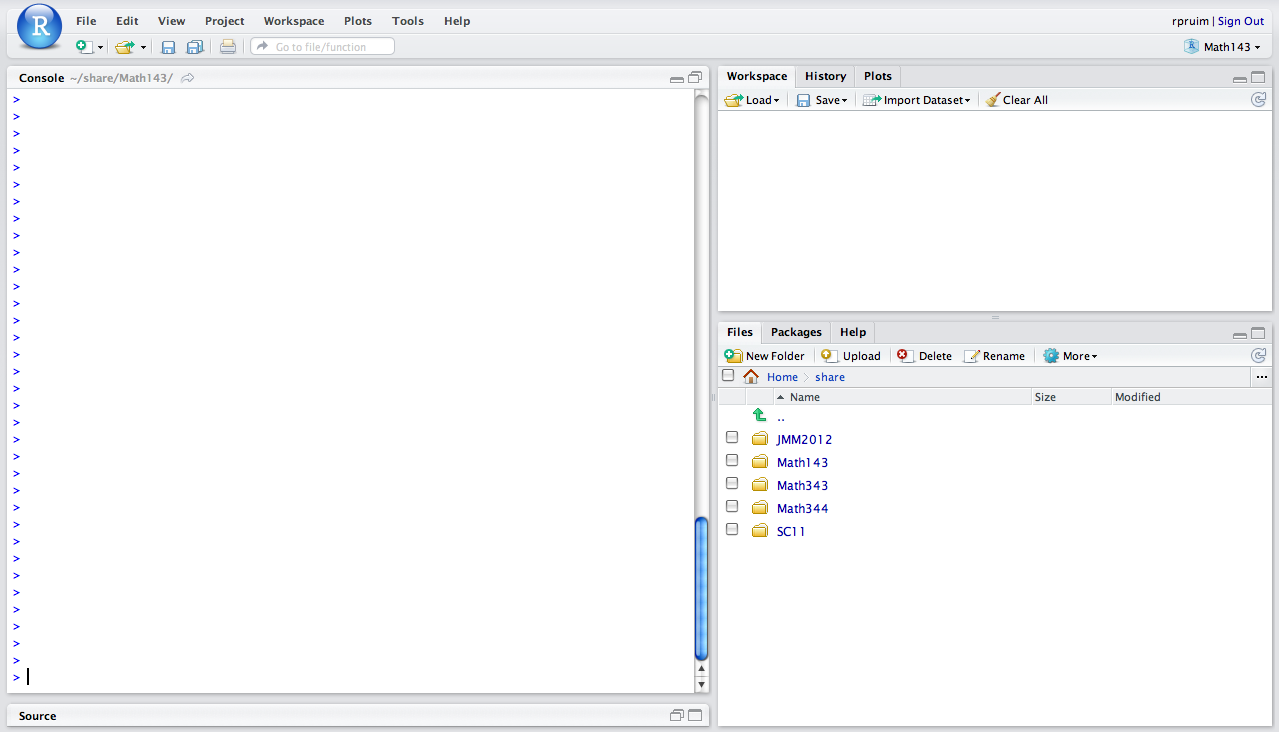
\includegraphics{images/RStudio-Welcome.png}
Figure 1: Welcome to RStudio

\hypertarget{using-r-as-a-calculator}{%
\subsection{Using R as a calculator}\label{using-r-as-a-calculator}}

Notice that RStudio divides its world into four panels. Several of the panels are further subdivided into multiple tabs.
The console panel is where we type commands that R will execute.

R can be used as a calculator. Try typing the following commands in the console panel.

\begin{Shaded}
\begin{Highlighting}[]
\DecValTok{5} \OperatorTok{+}\StringTok{ }\DecValTok{3}
\end{Highlighting}
\end{Shaded}

\begin{verbatim}
## [1] 8
\end{verbatim}

\begin{Shaded}
\begin{Highlighting}[]
\FloatTok{15.3} \OperatorTok{*}\StringTok{ }\FloatTok{23.4}
\end{Highlighting}
\end{Shaded}

\begin{verbatim}
## [1] 358.02
\end{verbatim}

\begin{Shaded}
\begin{Highlighting}[]
\KeywordTok{sqrt}\NormalTok{(}\DecValTok{16}\NormalTok{)}
\end{Highlighting}
\end{Shaded}

\begin{verbatim}
## [1] 4
\end{verbatim}

You can save values to named variables for later reuse

\begin{Shaded}
\begin{Highlighting}[]
\NormalTok{product =}\StringTok{ }\FloatTok{15.3} \OperatorTok{*}\StringTok{ }\FloatTok{23.4}       \CommentTok{# save result}
\NormalTok{product                     }\CommentTok{# show the result}
\end{Highlighting}
\end{Shaded}

\begin{verbatim}
## [1] 358.02
\end{verbatim}

\begin{Shaded}
\begin{Highlighting}[]
\NormalTok{product <-}\StringTok{ }\FloatTok{15.3} \OperatorTok{*}\StringTok{ }\FloatTok{23.4}      \CommentTok{# <- is assignment operator, same as =}
\NormalTok{product                     }
\end{Highlighting}
\end{Shaded}

\begin{verbatim}
## [1] 358.02
\end{verbatim}

\begin{Shaded}
\begin{Highlighting}[]
\FloatTok{15.3} \OperatorTok{*}\StringTok{ }\FloatTok{23.4}\NormalTok{ ->}\StringTok{ }\NormalTok{newproduct   }\CommentTok{# -> assigns to the right}
\NormalTok{newproduct}
\end{Highlighting}
\end{Shaded}

\begin{verbatim}
## [1] 358.02
\end{verbatim}

\begin{Shaded}
\begin{Highlighting}[]
\FloatTok{.5} \OperatorTok{*}\StringTok{ }\NormalTok{product                }\CommentTok{# half of the product}
\end{Highlighting}
\end{Shaded}

\begin{verbatim}
## [1] 179.01
\end{verbatim}

\begin{Shaded}
\begin{Highlighting}[]
\KeywordTok{log}\NormalTok{(product)                }\CommentTok{# (natural) log of the product}
\end{Highlighting}
\end{Shaded}

\begin{verbatim}
## [1] 5.880589
\end{verbatim}

\begin{Shaded}
\begin{Highlighting}[]
\KeywordTok{log10}\NormalTok{(product)              }\CommentTok{# base 10 log of the product}
\end{Highlighting}
\end{Shaded}

\begin{verbatim}
## [1] 2.553907
\end{verbatim}

\begin{Shaded}
\begin{Highlighting}[]
\KeywordTok{log}\NormalTok{(product, }\DataTypeTok{base =} \DecValTok{2}\NormalTok{)      }\CommentTok{# base 2 log of the product}
\end{Highlighting}
\end{Shaded}

\begin{verbatim}
## [1] 8.483896
\end{verbatim}

The semi-colon can be used to place multiple commands on one line. One frequent use of this is to save and print a value all in one go:

\begin{Shaded}
\begin{Highlighting}[]
\FloatTok{15.3} \OperatorTok{*}\StringTok{ }\FloatTok{23.4}\NormalTok{ ->}\StringTok{ }\NormalTok{product; product    }\CommentTok{# save result and show it}
\end{Highlighting}
\end{Shaded}

\begin{verbatim}
## [1] 358.02
\end{verbatim}

\hypertarget{getting-help-in-rstudio}{%
\section{Getting Help in RStudio}\label{getting-help-in-rstudio}}

\hypertarget{the-rstudio-help-system}{%
\subsection{The RStudio help system}\label{the-rstudio-help-system}}

There are several ways to get RStudio to help you when you forget something. Most objects in packages have help files that you can access by typing something like:

\begin{Shaded}
\begin{Highlighting}[]
\NormalTok{?bargraph}
\NormalTok{?histogram}
\NormalTok{?HELPrct}
\end{Highlighting}
\end{Shaded}

You can search the help system using

\begin{Shaded}
\begin{Highlighting}[]
\KeywordTok{help.search}\NormalTok{(}\StringTok{'Grand Rapids'}\NormalTok{)    }\CommentTok{# Does R know anything about Grand Rapids?}
\end{Highlighting}
\end{Shaded}

This can be useful if you don't know the name of the function or data set you are looking for.

\hypertarget{history}{%
\subsection{History}\label{history}}

If you know you have done something before, but can't remember how, you can search your history. The history tab shows a list of recently executed commands. There is also a search bar to help you find things from longer ago.

\hypertarget{error-messages}{%
\subsection{Error messages}\label{error-messages}}

When things go wrong, R tries to help you out by providing an error message. If you can't make sense of the message, you can try copying and pasting your command and the error message and sending to me in an email. One common error message is illustrated below.
\textless\textless error-message, purl=FALSE\textgreater\textgreater=
fred \textless- 23
frd
@
The object \texttt{frd} is not found because it was mistyped. It should have been \texttt{fred}. If you see an ``object not found'' message, check your typing and check to make sure that the necessary packages have been loaded.

\hypertarget{four-things-to-know-about-r}{%
\section{Four Things to Know About R}\label{four-things-to-know-about-r}}

Computers are great for doing complicated computations quickly, but you have to speak to them on their terms. Here are few things that will help you communicate with R

\begin{enumerate}
\def\labelenumi{(\arabic{enumi})}
\item
  R is case-sensitive

  If you mis-capitalize something in R it won't do what you want.
\item
  Functions in R use the following syntax:

\begin{Shaded}
\begin{Highlighting}[]
  \KeywordTok{functionname}\NormalTok{( argument1, argument2, ... )}
\end{Highlighting}
\end{Shaded}

  \begin{itemize}
  \item
    The arguments are \textbf{always} \emph{surrounded by (round) parentheses} and \emph{separated by commas}.
  \item
    Some functions (like \texttt{data()()}) have no required arguments, but you still need the parentheses.
  \item
    If you type a function name without the parentheses, you will see the \emph{code} for that function -- which probably isn't what you want at this point.
  \end{itemize}
\end{enumerate}

\begin{enumerate}
\def\labelenumi{(\arabic{enumi})}
\setcounter{enumi}{2}
\item
  TAB completion and arrows can improve typing speed and accuracy.

  If you begin a command and hit the TAB key, R will show you a list of possible ways to complete the command. If you hit TAB after the opening parenthesis of a function, it will show you the list of arguments it expects. The up and down arrows can be used to retrieve past commands.
\item
  If you get into some sort of mess typing (usually indicated by extra `\(+\)'
  signs along the left edge), you can hit the escape key to get back to
  a clean prompt.
\end{enumerate}

\hypertarget{data-in-r}{%
\section{Data in R}\label{data-in-r}}

\hypertarget{data-in-packages}{%
\subsection{Data in Packages}\label{data-in-packages}}

Most often, data sets in R are stored in a structure called a \textbf{data frame}. There are a number of data sets built into R and many more that come in various add on packages. The \textbf{\texttt{Lock5withR}} package, for example, contains all the data sets from our text book. In the book, data set names are printed in bold text.

You can see a list of them using

\begin{Shaded}
\begin{Highlighting}[]
\KeywordTok{data}\NormalTok{(}\DataTypeTok{package =} \StringTok{"Lock5withR"}\NormalTok{)}
\end{Highlighting}
\end{Shaded}

You can find a longer list of all data sets available in any loaded package using

\begin{Shaded}
\begin{Highlighting}[]
\KeywordTok{data}\NormalTok{()}
\end{Highlighting}
\end{Shaded}

\hypertarget{the-helprct-data-set}{%
\subsection{The HELPrct data set}\label{the-helprct-data-set}}

The {HELPrct} data frame from the \textbf{\texttt{mosaicData}} package contains data from the
Health Evaluation and Linkage to Primary Care randomized clinical trial.\\
You can find out more about the study and the data in this data frame by typing

\begin{Shaded}
\begin{Highlighting}[]
\NormalTok{?HELPrct}
\end{Highlighting}
\end{Shaded}

Among other things, this will tell us something about the subjects in this study:

\begin{quote}
Eligible subjects were adults, who spoke Spanish or English, reported
alcohol, heroin or cocaine as their first or second drug of choice, resided
in proximity to the primary care clinic to which they would be referred or
were homeless. Patients with established primary care relationships they
planned to continue, significant dementia, specific plans to leave the
Boston area that would prevent research participation, failure to provide
contact information for tracking purposes, or pregnancy were excluded.
\end{quote}

\begin{quote}
Subjects were interviewed at baseline during their detoxification stay and
follow-up interviews were undertaken every 6 months for 2 years.
\end{quote}

It is often handy to look at the first few rows of a data frame. It will show you the names of the variables and the kind of data in them:

\begin{Shaded}
\begin{Highlighting}[]
\KeywordTok{head}\NormalTok{(HELPrct)}
\end{Highlighting}
\end{Shaded}

That's plenty of variables to get us started with exploration of data.

\hypertarget{using-your-own-data}{%
\subsection{Using your own data}\label{using-your-own-data}}

\hypertarget{from-excel-or-google-to-r}{%
\subsubsection{From Excel or Google to R}\label{from-excel-or-google-to-r}}

So far we have been using data that lives in R packages. This has allowed us
to focus on things like how to make plots and create numerical summaries
without worrying too much about the data themselves. But if you are going to
do any of your own statistical analyses, then you will need to import your own
data into R and have some tools for manipulating the data once it is there.

Excel or Google spreadsheets are reasonable tools for entering (small) data
sets by hand and doing basic data tidying (organizing) and cleaning (correcting
errors). This section describes how to get data from a spreadsheet into R

\hypertarget{while-you-are-still-in-the-spreadsheet}{%
\subsubsection{While you are still in the spreadsheet}\label{while-you-are-still-in-the-spreadsheet}}

If you are creating your own data in a spreadsheet with the intent of bringing
into R (or some other statistical package) for analysis, it is important that
you design your spreadsheet appropriately. For most data sets this will mean

\begin{enumerate}
\def\labelenumi{\arabic{enumi}.}
\item
  The first row should contain variables names.

  These should be names that will work well in R This usually means they will be relatively short and avoid spaces and punctuation.
\item
  Each additional row corresponds to a case/observational unit.
\item
  Each column corresponds to a variable.
\item
  There is \textbf{nothing} else in the spreadsheet.

  Do not include notes to yourself, plots, numerical summaries, etc. These things can be kept in a separate worksheet, another file, your lab notebook, just not in the worksheet you are going to export.
\end{enumerate}

\hypertarget{exporting-to-csv}{%
\subsubsection{Exporting to csv}\label{exporting-to-csv}}

The comma separated values (csv) format has become a standard way of transferring data between programs. Both Google and Excel can export to this format, and R can import from this format. Once your dataare ready to go, export them to csv. Give the file a good name, and remember where you have put it.

\hypertarget{uploading-the-data-rstudio-server-only}{%
\subsubsection{Uploading the data (RStudio server only)}\label{uploading-the-data-rstudio-server-only}}

To get the data from your computer onto the server, you need to \textbf{upload} the data. (You can skip this step if you are working with a local copy of RStudio ) Uploading transfers a copy of your data from your computer onto the server (the ``cloud''). This is like uploading pictures to Facebook so you can later use them in posts or as a cover photo or tag your friends or whatever else once the photo is on Facebook.

To upload the data, go to the \textbf{Files} tab and click on \textbf{Upload}:

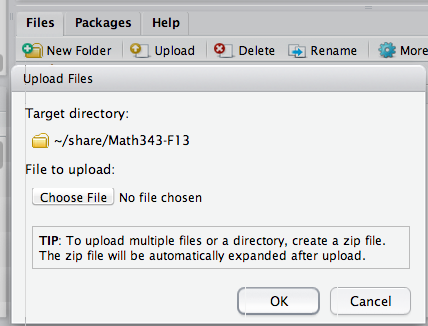
\includegraphics{images/Upload.png}

A window will pop up prompting you to browse to the file's location on your computer. Choose the file and it will upload to the server. You should see it appear in your file menu.

\hypertarget{importing-the-data-into-r}{%
\subsubsection{Importing the data into R}\label{importing-the-data-into-r}}

Now that the file is on the server, you can import it into R This takes place in the \textbf{Environment} tab. Once there, choose \textbf{Import Dataset} and then \textbf{From Text File\ldots{}}.\\
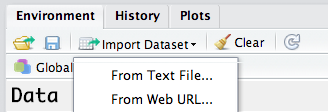
\includegraphics{images/Import1.png}

The instructions are pretty clear from there, but here are some things to watch for:

\begin{enumerate}
\tightlist
\item
  The default name for the data set is taken from the file name. If you used a very long file name, you will probably want to shorten this down. (But don't call it \texttt{Data} or something too generic either.) If the data are from the asters you have been tagging, perhaps call it \texttt{Asters}. If you are working with multiple data sets that deal with asters, add a bit more detail, perhaps \texttt{Asters01} or some such thing.
\item
  Be sure to select to use your first line as variable names (Heading = Yes).
\end{enumerate}

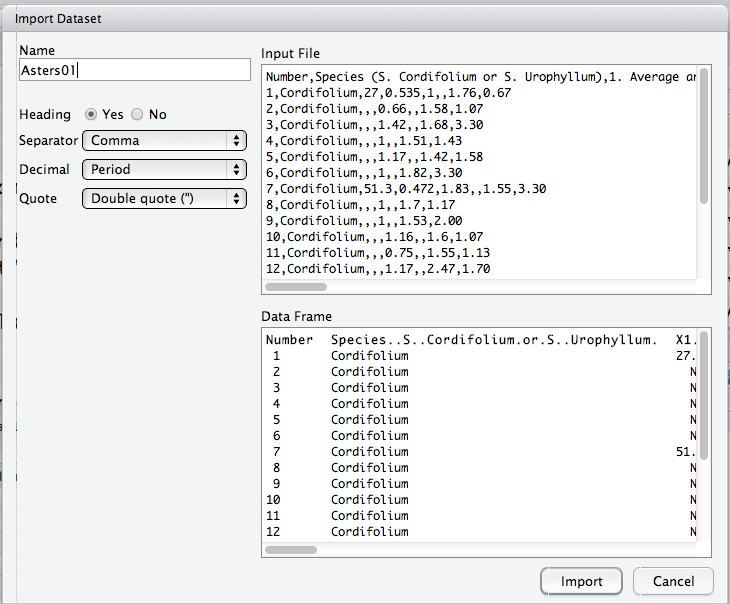
\includegraphics{images/Import2.png}

The data set should now be ready for use in R

\hypertarget{a-shortcut-for-google-spreadsheets}{%
\subsubsection{A shortcut for Google Spreadsheets}\label{a-shortcut-for-google-spreadsheets}}

The new \textbf{\texttt{googlesheets}} package provides a number of utilities
for reading and writing between R and Google sheets. At the time
of this writing, it is in active development and available via github.

\hypertarget{using-r-commands-to-read-a-data-file}{%
\subsubsection{Using R commands to read a data file}\label{using-r-commands-to-read-a-data-file}}

Even if you primarily use the RStudio interface to import data, it is good to know about the command line methods since these are required to import data into scripts, RMarkdown, and Rnw files. CSV files (and a few other types of files as well) can be read with

\begin{Shaded}
\begin{Highlighting}[]
\NormalTok{someData <-}\StringTok{ }\KeywordTok{read.file}\NormalTok{(}\StringTok{"file.csv"}\NormalTok{)}
\end{Highlighting}
\end{Shaded}

This can be used to read data directly from a URL as well. For example, here is some data from the US Census Bureau:

Many web sites provide data in csv format.\\
Here some examples:

\begin{enumerate}
\tightlist
\item
  \url{http://www.census.gov/} (Census Bureau data)
\item
  \url{http://www.ncdc.noaa.gov/data-access} (NOAA Weather and climate data)
\item
  \url{http://www.gapminder.org/data/} (Gapminder data)
\item
  \url{http://introcs.cs.princeton.edu/java/data/} has a number of data sets, some in csv format, collected from other places on the internet.
\item
  \url{http://www.exploredata.net/Downloads} has data from WHO, a genome expression study, and a microbiome study.
\end{enumerate}

But be aware that some of these files might need to be cleaned up a bit before
they are usable for statistics. Also, some internet files are very large and
may take a while to download. Many sites will give an indication of the size
of the data set so you know what you are in for. The better sites will
include links to a code book (a description of all the variables, units used,
how and when the data were collected, and any other information relevant to
interpreting the data). Such a document is available for the population data
loaded above. You can find it at
\url{http://www.census.gov/popest/data/national/totals/2012/files/NST-EST2012-alldata.pdf}

\hypertarget{missing-data}{%
\subsubsection{Missing Data}\label{missing-data}}

The {na.strings} argument can be used to specify codes for missing values. The following can be useful, for example:

\begin{Shaded}
\begin{Highlighting}[]
\NormalTok{someData <-}\StringTok{ }\KeywordTok{read.file}\NormalTok{(}\StringTok{'file.csv'}\NormalTok{, }\DataTypeTok{na.strings =} \StringTok{'.'}\NormalTok{)}
\NormalTok{someData <-}\StringTok{ }\KeywordTok{read.file}\NormalTok{(}\StringTok{'file.csv'}\NormalTok{, }\DataTypeTok{na.strings =} \StringTok{'-'}\NormalTok{)}
\end{Highlighting}
\end{Shaded}

because SAS uses a period (.) to code missing data, and some csv exporters use `\texttt{-}'. By default R reads these as string data, which forces the entire variable to be of character type instead of numeric.

\hypertarget{importing-other-kinds-of-data}{%
\subsubsection{Importing Other Kinds of Data}\label{importing-other-kinds-of-data}}

Many R packages provide the ability to load data from special data files. If you have data in some other format, there may well be
a package that makes it easy to load your data into R. For example, several packages (including \textbf{\texttt{readxl}}) provide the ability to read data
directly from Excel files without first saving the data as a csv file. If you make frequent use of Excel spreadsheets, you may find
this convenient. \textbf{\texttt{rdrop2}} provides the ability to manage data with Dropbox. And the \textbf{\texttt{foreign}} package provides functions
to read data from a wide range of other statistical packages.
But since these typically all know how to read and write csv files,
learning a workflow that goes through CSV is a broadly applicable skill.

\hypertarget{the-most-important-template}{%
\section{The Most Important Template}\label{the-most-important-template}}

Most of what we will do in this chapter makes use of a single R template:

\def\phbox#1{\fbox{`________`}}
\def\ttfbox#1{\fbox{#1}}

\[
\fbox{`________`} \; ( \; \fbox{`________`} \; \sim \; \fbox{`________`} \;, \; data = \fbox{`________`} \; )
\]

It is useful if we name the slots in this template:

\[
\fbox{goal} \; (  \;\fbox{y}  \;\sim  \;\fbox{x} \;, \; \texttt{data}=\fbox{mydata} \; )
\]

Actually, there are some variations on this template:

\begin{Shaded}
\begin{Highlighting}[]
\CommentTok{### Simpler version -- for just one variable}
\KeywordTok{goal}\NormalTok{( }\OperatorTok{~}\StringTok{ }\NormalTok{x, }\DataTypeTok{data =}\NormalTok{ mydata )}

\CommentTok{### Fancier version: }
\KeywordTok{goal}\NormalTok{( y }\OperatorTok{~}\StringTok{ }\NormalTok{x }\OperatorTok{|}\StringTok{ }\NormalTok{z , }\DataTypeTok{data =}\NormalTok{ mydata )}
 
\CommentTok{### Unified version: }
\KeywordTok{goal}\NormalTok{( formula , }\DataTypeTok{data =}\NormalTok{ mydata )}
\end{Highlighting}
\end{Shaded}

To use the template (we'll call it the formula template because there is always
a formula involved), you just need to know what goes in each slot. This can be determined by asking yourself two questions:

\begin{enumerate}
\def\labelenumi{\arabic{enumi}.}
\tightlist
\item
  What do you want R to do?

  \begin{itemize}
  \tightlist
  \item
    this determines what function to use (goal).
  \end{itemize}
\item
  What must R know to do that?

  \begin{itemize}
  \tightlist
  \item
    this determines the inputs to the function
  \item
    for describing data, must must identify \emph{which data frame} and \emph{which variable(s)}.
  \end{itemize}
\end{enumerate}

Let's try an example. Suppose we want to make this plot

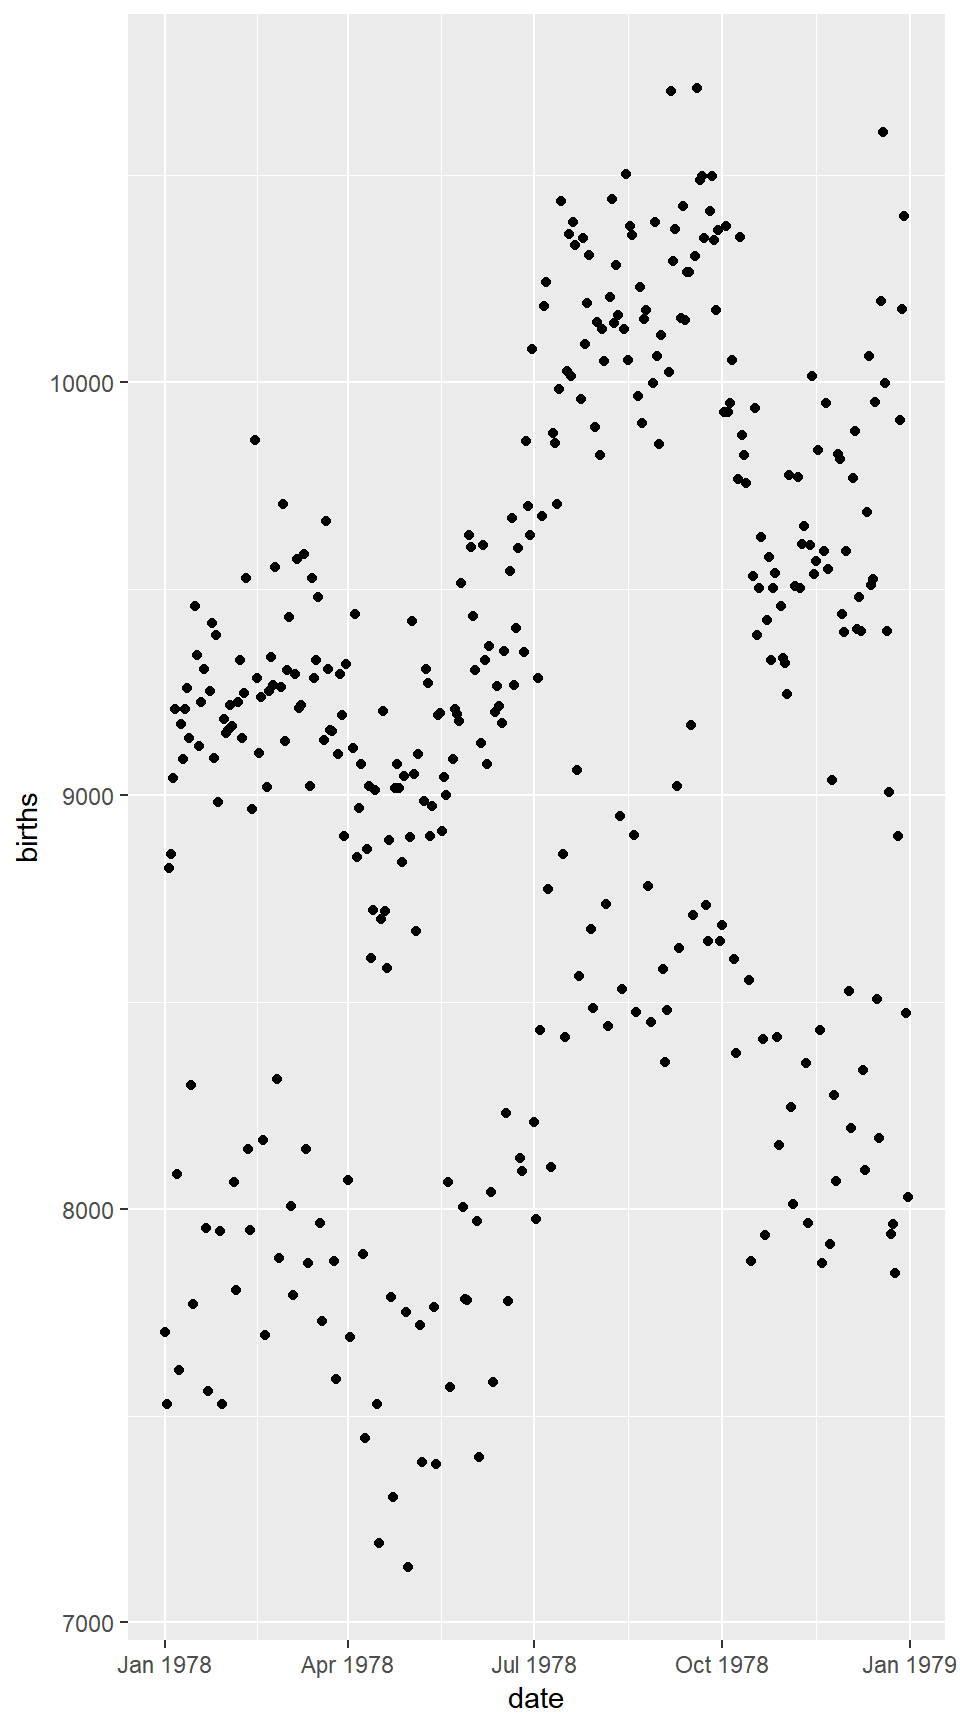
\includegraphics[width=0.65\linewidth]{Lock5WithR_files/figure-latex/unnamed-chunk-8-1}

\begin{enumerate}
\def\labelenumi{\arabic{enumi}.}
\item
  What is our goal?

  Our goal is to make a scatter plot. The function that does this is called \texttt{xyplot()()}. That takes care of the first slot.
\item
  What does R need to know to do this?

  It needs to know what data set to use, and which varialbes to use on the x and y axes. These data are in the {Births78} data set in the \textbf{\texttt{mosaicData}} package. Let's take a quick look at the data:
\end{enumerate}

\begin{Shaded}
\begin{Highlighting}[]
\KeywordTok{require}\NormalTok{(mosaicData)  }\CommentTok{# load the package that contains our data set}
\KeywordTok{head}\NormalTok{(Births78)}
\end{Highlighting}
\end{Shaded}

\begin{verbatim}
##         date births wday year month day_of_year day_of_month day_of_week
## 1 1978-01-01   7701  Sun 1978     1           1            1           1
## 2 1978-01-02   7527  Mon 1978     1           2            2           2
## 3 1978-01-03   8825  Tue 1978     1           3            3           3
## 4 1978-01-04   8859  Wed 1978     1           4            4           4
## 5 1978-01-05   9043  Thu 1978     1           5            5           5
## 6 1978-01-06   9208  Fri 1978     1           6            6           6
\end{verbatim}

We want the date on the x-axis and the number of births on the y axis, so
the full command is

\begin{Shaded}
\begin{Highlighting}[]
\KeywordTok{xyplot}\NormalTok{(births }\OperatorTok{~}\StringTok{ }\NormalTok{date, }\DataTypeTok{data =}\NormalTok{ Births78)}
\end{Highlighting}
\end{Shaded}

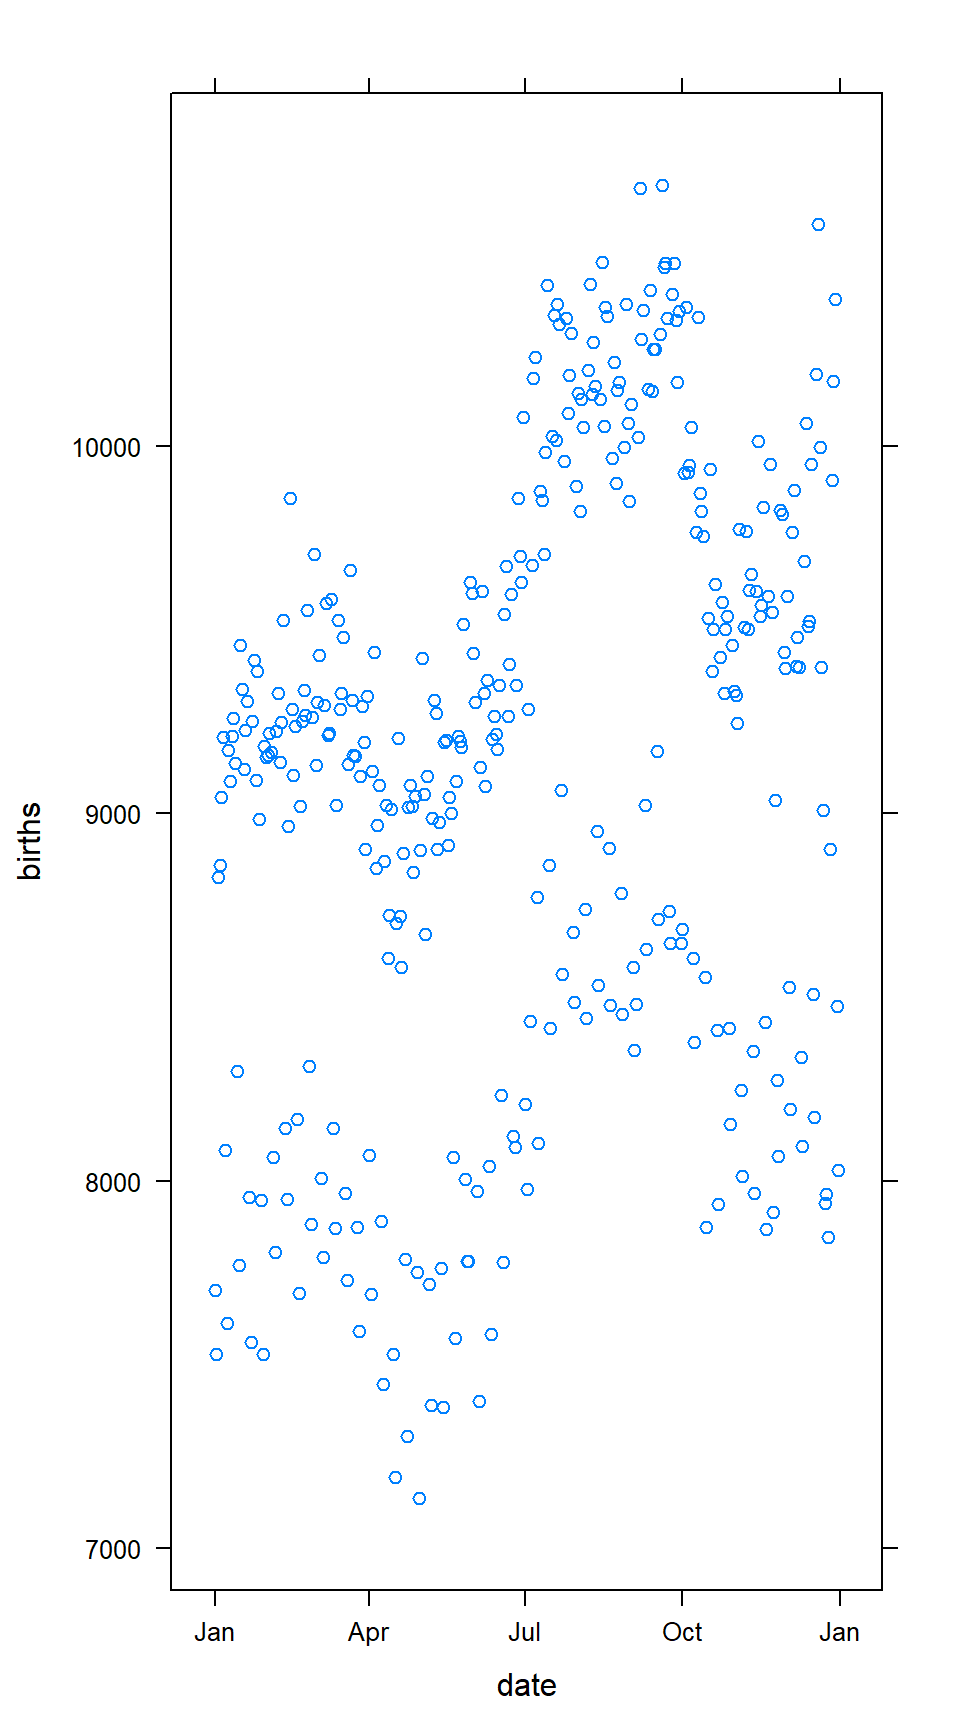
\includegraphics[width=0.65\linewidth]{Lock5WithR_files/figure-latex/births-scatterplot-1}

This same template can be used for a wide variety of graphical and
numerical summaries. For example, to compute the mean number of births, we can
change \texttt{xyplot()()} to \texttt{mean()()} and provide {births}
but not {date}:

\begin{Shaded}
\begin{Highlighting}[]
\KeywordTok{mean}\NormalTok{( }\OperatorTok{~}\StringTok{ }\NormalTok{births, }\DataTypeTok{data =}\NormalTok{ Births78)}
\end{Highlighting}
\end{Shaded}

\begin{verbatim}
## [1] 9132.162
\end{verbatim}

Notice that when there is only one variable, it goes on the right side of the
wiggle (\textasciitilde).

We'll see more examples of this template as we go along.

\hypertarget{manipulating-your-data}{%
\section{Manipulating your data}\label{manipulating-your-data}}

\hypertarget{creating-a-subset}{%
\subsection{Creating a subset}\label{creating-a-subset}}

The \texttt{filter()()} command can be used to create subsets. The population
data set we downloaded has population for states and various other regions. If we
just want the states, we can select the items where the {State} variable is
greater than 0. (Notice the double equals for testing equality.)

That two states too many. We can scan the list to see what else is in there.

The two extras are Washington, DC and Peurto Rico.

\hypertarget{choosing-specific-columns}{%
\subsection{Choosing specific columns}\label{choosing-specific-columns}}

\texttt{filter()()} chooses rows from a data frame. \texttt{select()()} selects
columns. This can be handy if you have a data set with many more variables than you are interested in. Let's pick just a handful from the {Population} data
set.

\hypertarget{dropping-variables}{%
\subsection{Dropping Variables}\label{dropping-variables}}

Sometimes it is easier to think about dropping variables.
We can use \texttt{select()()} for this as well:

\begin{Shaded}
\begin{Highlighting}[]
\NormalTok{iris2 <-}\StringTok{ }\KeywordTok{select}\NormalTok{(iris, }\OperatorTok{-}\StringTok{ }\NormalTok{Sepal.Width, }\OperatorTok{-}\StringTok{ }\NormalTok{Sepal.Length)  }\CommentTok{# the minus sign means drop }
\KeywordTok{head}\NormalTok{(iris2, }\DecValTok{3}\NormalTok{)}
\end{Highlighting}
\end{Shaded}

\begin{verbatim}
##   Petal.Length Petal.Width Species
## 1          1.4         0.2  setosa
## 2          1.4         0.2  setosa
## 3          1.3         0.2  setosa
\end{verbatim}

\hypertarget{creating-new-variables}{%
\subsection{Creating new variables}\label{creating-new-variables}}

We can add a new variable to data set using \texttt{mutate()()}:
--\textgreater{}

Generally, it is a good idea to keep raw data (like {Sepal.Length} and {Sepal.Width} in your data file, but let R do the computation of derived variables for you. Among other advantages, if you ever fix an error in a {Sepal.Length} measurement, you don't have to worry about remembering to also recompute the ratio. Futhermore, your R code documents how the derived value was computed.

\hypertarget{saving-data}{%
\subsection{Saving Data}\label{saving-data}}

\texttt{write.csv()()} can be used to save data from R into csv formatted files. This can be useful for exporting to some other program.

Data can also be saved in native R format. Saving data sets (and other R objects) using \texttt{save()()} has some advantages over other file formats:
\#. Complete information about the objects is saved, including attributes.
\#. Data saved this way takes less space and loads much more quickly.
\#. Multiple objects can be saved to and loaded from a single file.
The downside is that these files are only readable in R

For more on importing and exporting data, especially from other formats, see the \emph{R Data Import/Export} manual available on \href{http://cran.r-project.org/manuals.html}{CRAN}.

\hypertarget{merging-datasets}{%
\subsection{Merging datasets}\label{merging-datasets}}

The {fusion1} data frame in the \textbf{\texttt{fastR}} package contains genotype information for a SNP (single nucleotide polymorphism) in the gene \emph{TCF7L2}. The {pheno} data frame contains phenotypes (including type 2 diabetes case/control status) for an intersecting set of individuals. We can merge these together to explore the association between genotypes and phenotypes using merge().

\begin{Shaded}
\begin{Highlighting}[]
\KeywordTok{head}\NormalTok{(fusion1, }\DecValTok{3}\NormalTok{)}
\end{Highlighting}
\end{Shaded}

\begin{verbatim}
##      id     marker markerID allele1 allele2 genotype Adose Cdose Gdose
## 1  9735 RS12255372        1       3       3       GG     0     0     2
## 2 10158 RS12255372        1       3       3       GG     0     0     2
## 3  9380 RS12255372        1       3       4       GT     0     0     1
##   Tdose
## 1     0
## 2     0
## 3     1
\end{verbatim}

\begin{Shaded}
\begin{Highlighting}[]
\KeywordTok{head}\NormalTok{(pheno, }\DecValTok{3}\NormalTok{)}
\end{Highlighting}
\end{Shaded}

\begin{verbatim}
##     id     t2d      bmi sex      age smoker chol waist weight height
## 1 1002    case 32.85994   F 70.76438 former 4.57 112.0   85.6  161.4
## 2 1009    case 27.39085   F 53.91896  never 7.32  93.5   77.4  168.1
## 3 1012 control 30.47048   M 53.86161 former 5.02 104.0   94.6  176.2
##         whr sbp dbp
## 1 0.9867841 135  77
## 2 0.9396985 158  88
## 3 0.9327354 143  89
\end{verbatim}

\begin{Shaded}
\begin{Highlighting}[]
\CommentTok{# merge fusion1 and pheno keeping only id's that are in both}
\NormalTok{fusion1m <-}\StringTok{ }\KeywordTok{merge}\NormalTok{(fusion1, pheno, }\DataTypeTok{by.x =} \StringTok{'id'}\NormalTok{, }\DataTypeTok{by.y =} \StringTok{'id'}\NormalTok{, }\DataTypeTok{all.x =} \OtherTok{FALSE}\NormalTok{, }\DataTypeTok{all.y =} \OtherTok{FALSE}\NormalTok{)}
\KeywordTok{head}\NormalTok{(fusion1m, }\DecValTok{3}\NormalTok{)}
\end{Highlighting}
\end{Shaded}

\begin{verbatim}
##     id     marker markerID allele1 allele2 genotype Adose Cdose Gdose
## 1 1002 RS12255372        1       3       3       GG     0     0     2
## 2 1009 RS12255372        1       3       3       GG     0     0     2
## 3 1012 RS12255372        1       3       3       GG     0     0     2
##   Tdose     t2d      bmi sex      age smoker chol waist weight height
## 1     0    case 32.85994   F 70.76438 former 4.57 112.0   85.6  161.4
## 2     0    case 27.39085   F 53.91896  never 7.32  93.5   77.4  168.1
## 3     0 control 30.47048   M 53.86161 former 5.02 104.0   94.6  176.2
##         whr sbp dbp
## 1 0.9867841 135  77
## 2 0.9396985 158  88
## 3 0.9327354 143  89
\end{verbatim}

In this case, since the values are the same for each data frame, we could collapse {by.x} and {by.y} to {by} and collapse {all.x} and {all.y} to {all}. The first of these specifies which column(s) to use to identify matching cases. The second indicates whether cases in one data frame that do not appear in the other should be kept (\texttt{TRUE}) or dropped (filling in \texttt{NA} as needed) or dropped from the merged data frame.

Now we are ready to begin our analysis.

\begin{Shaded}
\begin{Highlighting}[]
\KeywordTok{tally}\NormalTok{(}\OperatorTok{~}\NormalTok{t2d }\OperatorTok{+}\StringTok{ }\NormalTok{genotype, fusion1m)}
\end{Highlighting}
\end{Shaded}

\begin{verbatim}
##          genotype
## t2d        GG  GT  TT
##   case    737 375  48
##   control 835 309  27
\end{verbatim}

\hypertarget{using-r-markdown}{%
\section{Using R Markdown}\label{using-r-markdown}}

Although you can export plots from RStudio for use in other applications, there is another way of preparing documents that has many advantages.\\
RStudio provides several ways to create documents that include text, R code, R output, graphics, even mathematical notation all in one document. The simplest of these is R Markdown.

To create a new R Markdown document, go to ``File'', ``New'', then ``R Markdown'':
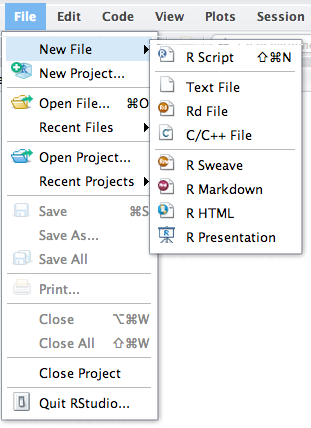
\includegraphics{images/NewRMarkdown.png}

When you do this, a file editing pane will open with a template inserted. If you click on \texttt{Knit\ HTML",\ \textbackslash{}RStudio\textbackslash{}\ will\ turn\ this\ into\ an\ HTML\ file\ and\ display\ it\ for\ you.\ \ Give\ it\ a\ try.\ You\ will\ be\ asked\ to\ name\ your\ file\ if\ you\ haven\textquotesingle{}t\ already\ done\ so.\ \ If\ you\ are\ using\ the\ \textbackslash{}RStudio\textbackslash{}\ server\ in\ a\ browser,\ then\ your\ file\ will\ live\ on\ the\ server\ (}in the cloud'') rather than on your computer.

If you look at the template file you will see that the file has two kinds of sections. Some of this file is just normal text (with some extra symbols to make things bold, add in headings, etc.) You can get a list of all of these mark up options by selecting the ``Mardown Quick Reference" in the question mark menu.

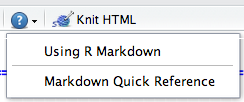
\includegraphics{images/MardownQuickReference.png}

The second type of section is an R code chunk. These are colored differently to make them easier to see. You can insert a new code chunk by selecting ``Insert Chunk'' from the ``Chunks''
menu:

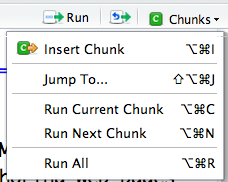
\includegraphics{images/InsertChunk.png}
(You can also type \texttt{\{r\}!\ to\ begin\ and}! to end the code chunk if you would rather type.) You can put any R code in these code chunks and the results (text output or graphics) as well as the R code will be displayed in your HTML file.

There are options to do things like (a) run R code without displaying it, (b) run R code without
displaying the output, (c) controling size of plots, etc., etc.\\
But for starting out, this is really all you need to know.

\hypertarget{r-markdown-files-must-be-self-contained}{%
\subsection{R Markdown files must be self-contained}\label{r-markdown-files-must-be-self-contained}}

R Markdown files do not have access to things you have done in your console. (This is good, else your document would change based on things not in the file.) This means that you must explicitly load data, and require packages \emph{in the R Markdown file} in order to use them. In this class, this means that most of your R Markdown files will have a chunk near the beginning that includes

\begin{Shaded}
\begin{Highlighting}[]
\KeywordTok{require}\NormalTok{(mosaic)        }\CommentTok{# load the mosaic package}
\KeywordTok{require}\NormalTok{(Lock5withR)    }\CommentTok{# get data sets from the book}
\end{Highlighting}
\end{Shaded}

The \textbf{\texttt{mosaic}} package provides some templates that are available if you choose ``from template'' when creating an RMarkdown file in RStudio .
Among other things, this will insert the code required to load the \textbf{\texttt{mosaic}} package, change some default settings, and include a reminder to
load any additional packages you will be using.

\hypertarget{output-formats}{%
\subsection{Output formats}\label{output-formats}}

RStudio makes it easy to generate HTML, PDF, or Word documents from your RMarkdown. Just remember that if you edit any of these files after you generate them
with RMarkdown, then you will need to redo those edits if you ever go back and change the RMarkdown file, but if you change the RMarkdown file, one click will
generate the new HTML, PDF, or Word document. (There are even ways to get it to generate all three in one go;
see the \texttt{render()()} function in the \textbf{\texttt{rmarkdown}} package.) So it is best to keep you editing to the RMarkdown document as much as possible.

\hypertarget{statistics-answering-questions-with-data}{%
\section{Statistics: Answering Questions With Data}\label{statistics-answering-questions-with-data}}

This is a course primarily about statistics, but what exactly is \emph{statistics}? In other words, what is this course about? \footnote{As we will see, the words \emph{statistic} and \emph{statistics} get used in more than one way. More on that later.}

Here are some definitions of statistics from other people:

\begin{enumerate}
\item
  a collection of procedures and principles for gaining information in
  order to make decisions when faced with
  uncertainty (J. Utts \citet{Utts:2005:SeeingThroughStats}),
\item
  a way of taming uncertainty, of turning raw data into arguments that
  can resolve profound questions (T. Amabile \citet{AgainstAllOdds:video}),
\item
  the science of drawing conclusions from data with the aid of the
  mathematics of probability
  (S. Garfunkel \citet{ForAllPracticalPurposes:video}),
  \#. the explanation of variation in the context of what remains unexplained
  (D. Kaplan \citet{kaplan-modeling}),
\item
  the mathematics of the collection, organization, and interpretation of
  numerical data, especially the analysis of a population's characteristics by
  inference from sampling
  (American Heritage Dictionary \citet{AmHerDictionary:1982}).
\end{enumerate}

Here's a simpler definition:

\begin{verbatim}
    Statistics is the science of answering questions with data.
\end{verbatim}

This definition gets at two important elements of the longer definitions above:

\hypertarget{data-the-raw-material}{%
\subsection{Data -- the raw material}\label{data-the-raw-material}}

data
Data are the raw material for doing statistics. We will learn more about different types of data, how to collect data, and how to summarize data as we go along.

\hypertarget{information-the-goal}{%
\subsection{Information -- the goal}\label{information-the-goal}}

The goal of doing statistics is to gain some information or to make a decision -- that is, to answer some question.

Statistics is useful because it helps us answer questions like the following:
\footnote{The opening pages of each chapter of our book include many more questions.}

\begin{enumerate}
\tightlist
\item
  Which of two treatment plans leads to the best clinical outcomes?
\item
  Are men or women more successful at quitting smoking? And does it matter which smoking cessation program they use?
\item
  Is my cereal company complying with regulations about the amount of cereal in its cereal boxes?
  In this sense, statistics is a science -- a method for obtaining new knowledge.
  Our simple definition is light on describing the context in which this takes place.
  So let's add two more important aspects of statistics.
\end{enumerate}

\hypertarget{uncertainty-the-context}{%
\subsection{Uncertainty -- the context}\label{uncertainty-the-context}}

randomness
The tricky thing about statistics is the uncertainty involved. If we measure one box of cereal, how do we know that all the others are similarly filled? If every box of cereal were identical and every measurement perfectly exact, then one measurement would suffice. But the boxes may differ from one another, and even if we measure the same box multiple times, we may get different answers to the question
\emph{How much cereal is in the box?}

So we need to answer questions like
\emph{How many boxes should we measure?}
and
\emph{How many times should we measure each box?}
Even so, there is no answer to these questions
that will give us absolute certainty.
So we need to answer questions like
\emph{How sure do we need to be?}

\hypertarget{probability-the-tool}{%
\subsection{Probability -- the tool}\label{probability-the-tool}}

In order to answer a question like \emph{How sure do we need to be?}, we need some way of measuring our level of certainty. This is where mathematics enters into statistics. Probability is the area of mathematics that deals with reasoning about uncertainty.

\hypertarget{a-first-example-the-lady-tasting-tea}{%
\section{A First Example: The Lady Tasting Tea}\label{a-first-example-the-lady-tasting-tea}}

There is a famous story about a lady who claimed that tea with milk tasted different depending on whether the milk was added to the tea or the tea added to the milk. The story is famous because of the setting in which she made this claim. She was attending a party in Cambridge, England, in the \(1920\)s. Also in attendance were a number of university dons and their wives. The scientists in attendance scoffed at the woman and her claim. What, after all, could be the difference?

Fisher, R. A.
All the scientists but one, that is. Rather than simply dismiss the woman's claim, he proposed that they decide how one should \emph{test} the claim. The tenor of the conversation changed at this suggestion, and the scientists began to discuss how the claim should be tested. Within a few minutes cups of tea with milk had been prepared and presented to the woman for tasting.

Let's take this simple example as a prototype for a statistical study.
What steps are involved?\\

\begin{enumerate}
\item
  Determine the question of interest.

  Just what is it we want to know? It may take some effort to make a vague idea precise. The precise questions may not exactly correspond to our vague questions, and the very exercise of stating the question precisely may modify our question. Sometimes we cannot come up with any way to answer the question we really want to answer, so we have to live with some other question that is not exactly what we wanted but is something we can study and will (we hope) give us some information about our original question.

  In our example this question seems fairly easy to state: Can the lady tell the difference between the two tea preparations? But we need to refine this question. For example, are we asking if she \emph{always} correctly identifies cups of tea or merely if she does better than we could do ourselves (by guessing)?
\item
  Determine the \textbf{population}.

  Just who or what do we want to know about? Are we only interested in this one woman or women in general or only women who claim to be able to distinguish tea preparations?
\item
  Select \textbf{measurements}.

  We are going to need some data. We get our data by making some measurements. These might be physical measurements with some device (like a ruler or a scale). But there are other sorts of measurements too, like the answer to a question on a form. Sometimes it is tricky to figure out just what to measure. (How do we measure happiness or intelligence, for example?) Just how we do our measuring will have important consequences for the subsequent statistical analysis. The recorded values of these measurements are called \textbf{variables} (because the values vary from one individual to another).

  In our example, a measurement may consist of recording for a given cup of tea whether the woman's claim is correct or incorrect.
\item
  Determine the \textbf{sample}.

  Usually we cannot measure every individual in our population; we have to select some to measure. But how many and which ones? These are important questions that must be answered. Generally speaking, bigger is better, but it is also more expensive. Moreover, no size is large enough if the sample is selected inappropriately.

  Suppose we gave the lady one cup of tea. If she correctly identifies
  the mixing procedure, will we be convinced of her claim? She might just
  be guessing; so we should probably have her taste more than one
  cup. Will we be convinced if she correctly identifies \(5\) cups? \(10\) cups?
  \(50\) cups?

  What if she makes a mistake? If we present her with \(10\) cups and she
  correctly identifies \(9\) of the \(10\), what will we conclude?
  A success rate of \(90\)\% is, it seems,
  much better than just guessing, and anyone can make a mistake now and then.
  But what if she correctly identifies \(8\) out of \(10\)? \(80\) out of \(100\)?

  And how should we prepare the cups? Should we make \(5\) each way?
  Does it matter if we tell the woman that there are \(5\) prepared
  each way?
  Should we flip a coin to decide even if that means we might end
  up with \(3\) prepared one way and \(7\) the other way?\\
  Do any of these differences matter?
\item
  Make and record the measurements.

  Once we have the design figured out, we have to do the legwork of
  data collection. This can be a time-consuming and tedious process.
  In the case of the lady tasting tea, the scientists decided to
  present her with ten cups of tea which were quickly prepared.
  A study of public opinion may require many thousands of phone calls or
  personal interviews.
  In a laboratory setting, each measurement might be the result
  of a carefully performed laboratory experiment.
\item
  Organize the data.

  Once the data have been collected, it is often necessary or useful
  to organize them. Data are typically stored in spreadsheets or
  in other formats that are convenient for processing with
  statistical packages. Very large data sets are often stored in
  databases.

  Part of the organization of the data may involve producing graphical and
  numerical summaries of the data. These summaries may give us initial
  insights into our questions or help us detect errors that may have occurred
  to this point.
\item
  Draw conclusions from data.

  Once the data have been collected, organized, and analyzed, we need
  to reach a conclusion.
  Do we believe the woman's claim? Or do we think she is merely guessing?\\
  How sure are we that this
  conclusion is correct?

  Eventually we will
  learn a number of important and frequently used methods for
  drawing inferences from data. More importantly, we will learn
  the basic framework used for such procedures so that it should
  become easier and easier to learn new procedures as we become
  familiar with the framework.
\item
  Produce a report.

  Typically the results of a statistical study are reported in
  some manner. This may be as a refereed article in an academic
  journal, as an internal report to a company, or as a solution
  to a problem on a homework assignment. These reports may themselves
  be further distilled into press releases, newspaper articles,
  advertisements, and the like. The mark of a good report
  is that it provides the essential information about each
  of the steps of the study.

  As we go along, we will learn some of the standard terminology and
  procedures that you are likely to see in basic statistical reports and
  will gain a framework for learning more.\\
\end{enumerate}

At this point, you may be wondering who the innovative scientist was and what the results of the experiment were. Fisher, R. A.
The scientist was R. A. Fisher, who first described this situation as a pedagogical example in his 1925 book on statistical methodology \citet{Fisher:1925:Methods}. Fisher developed statistical methods that are among the most important and widely used methods to this day, and most of his applications were biological.

\hypertarget{coins-and-cups}{%
\section{Coins and Cups}\label{coins-and-cups}}

You might also be curious about how the experiment came out. How many cups of tea were prepared? How many did the woman correctly identify? What was the conclusion?

Fisher never says. In his book he is interested in the method, not the particular results. But let's suppose we decide to test the lady with ten cups of tea. We'll flip a coin to decide which way to prepare the cups. If we flip a head, we will pour the milk in first; if tails, we put the tea in first. Then we present the ten cups to the lady and have her state which ones she thinks were prepared each way.

It is easy to give her a score (9 out of 10, or 7 out of 10, or whatever it happens to be). It is trickier to figure out what to do with her score. Even if she is just guessing and has no idea, she could get lucky and get quite a few correct -- maybe even all 10. But how likely is that?

Let's try an experiment. I'll flip 10 coins. You guess which are heads and which are tails, and we'll see how you do.

\(\vdots\)

Comparing with your classmates, we will undoubtedly see that some of you did better and others worse.

Now let's suppose the lady gets 9 out of 10 correct. That's not perfect, but it is better than we would expect for someone who was just guessing. On the other hand, it is not impossible to get 9 out of 10 just by guessing. So here is Fisher's great idea: Let's figure out how hard it is to get 9 out of 10 by guessing. If it's not so hard to do, then perhaps that's just what happened, so we won't be too impressed with the lady's tea tasting ability. On the other hand, if it is really unusual to get 9 out of 10 correct by guessing, then we will have some evidence that she must be able to tell something.

But how do we figure out how unusual it is to get 9 out of 10 just by guessing? We'll learn another method later, but for now, let's just flip a bunch of coins and keep track. If the lady is just guessing, she might as well be flipping a coin.

So here's the plan. We'll flip 10 coins. We'll call the heads correct guesses and the tails incorrect guesses. Then we'll flip 10 more coins, and 10 more, and 10 more, and \ldots{} That would get pretty tedious. Fortunately, computers are good at tedious things, so we'll let the computer do the flipping for us using a tool in the \textbf{\texttt{mosaic}} package. This package is already installed in our RStudio server. If you are running your own installation of R you can install \textbf{\texttt{mosaic}} using the following command:

\begin{Shaded}
\begin{Highlighting}[]
\KeywordTok{install.packages}\NormalTok{(}\StringTok{"mosaic"}\NormalTok{)}
\end{Highlighting}
\end{Shaded}

The \texttt{rflip()()} function can flip one coin

\begin{Shaded}
\begin{Highlighting}[]
\KeywordTok{require}\NormalTok{(mosaic)}
\KeywordTok{rflip}\NormalTok{()}
\end{Highlighting}
\end{Shaded}

\begin{verbatim}
## 
## Flipping 1 coin [ Prob(Heads) = 0.5 ] ...
## 
## T
## 
## Number of Heads: 0 [Proportion Heads: 0]
\end{verbatim}

or a number of coins

\begin{Shaded}
\begin{Highlighting}[]
\KeywordTok{rflip}\NormalTok{(}\DecValTok{10}\NormalTok{)}
\end{Highlighting}
\end{Shaded}

\begin{verbatim}
## 
## Flipping 10 coins [ Prob(Heads) = 0.5 ] ...
## 
## H H H T T T T H H H
## 
## Number of Heads: 6 [Proportion Heads: 0.6]
\end{verbatim}

and show us the results.

Typing \texttt{rflip(10)} a bunch of times is almost as tedious as flipping all those coins. But it is not too hard to tell R to \texttt{do()()} this a bunch of times.

\begin{Shaded}
\begin{Highlighting}[]
\KeywordTok{do}\NormalTok{(}\DecValTok{2}\NormalTok{) }\OperatorTok{*}\StringTok{ }\KeywordTok{rflip}\NormalTok{(}\DecValTok{10}\NormalTok{)}
\end{Highlighting}
\end{Shaded}

\begin{verbatim}
##    n heads tails prop
## 1 10     5     5  0.5
## 2 10     6     4  0.6
\end{verbatim}

Let's get R to \texttt{do()()} it for us 10,000 times and make a table of the results.

\begin{Shaded}
\begin{Highlighting}[]
\NormalTok{Flips <-}\StringTok{ }\KeywordTok{do}\NormalTok{(}\DecValTok{10000}\NormalTok{) }\OperatorTok{*}\StringTok{ }\KeywordTok{rflip}\NormalTok{(}\DecValTok{10}\NormalTok{)}
\KeywordTok{tally}\NormalTok{(}\OperatorTok{~}\NormalTok{heads, }\DataTypeTok{data =}\NormalTok{ Flips)}
\end{Highlighting}
\end{Shaded}

\begin{verbatim}
## heads
##    0    1    2    3    4    5    6    7    8    9   10 
##    5  102  467 1203 2048 2470 2035 1140  415  108    7
\end{verbatim}

\begin{Shaded}
\begin{Highlighting}[]
\KeywordTok{tally}\NormalTok{(}\OperatorTok{~}\NormalTok{heads, }\DataTypeTok{data =}\NormalTok{ Flips, }\DataTypeTok{format =} \StringTok{'percent'}\NormalTok{)}
\end{Highlighting}
\end{Shaded}

\begin{verbatim}
## heads
##     0     1     2     3     4     5     6     7     8     9    10 
##  0.05  1.02  4.67 12.03 20.48 24.70 20.35 11.40  4.15  1.08  0.07
\end{verbatim}

\begin{Shaded}
\begin{Highlighting}[]
\KeywordTok{tally}\NormalTok{(}\OperatorTok{~}\NormalTok{heads, }\DataTypeTok{data =}\NormalTok{ Flips, }\DataTypeTok{format =} \StringTok{'proportion'}\NormalTok{)}
\end{Highlighting}
\end{Shaded}

\begin{verbatim}
## heads
##      0      1      2      3      4      5      6      7      8      9 
## 0.0005 0.0102 0.0467 0.1203 0.2048 0.2470 0.2035 0.1140 0.0415 0.0108 
##     10 
## 0.0007
\end{verbatim}

You might be surprised to see that the number of correct guesses is exactly 5 (half of the 10 tries) only
25\%
of the time. But most of the results are quite close to 5 correct.
67\% of the results are
4, 5, or 6, for example.
And 1\% of the results are between 3 and 7 (inclusive). But getting 8 correct is a bit unusual, and getting 9 or 10 correct is even
more unusual.

So what do we conclude? It is possible that the lady could get 9 or 10 correct just by guessing, but it is not very likely (it only happened in about
1.2\% of our simulations).
So \emph{one of two things must be true}:

\begin{enumerate}
\tightlist
\item
  The lady got unusually ``lucky'', or
\item
  The lady is not just guessing.
\end{enumerate}

Although Fisher did not say how the experiment came out, others have reported that the lady correctly identified all 10 cups!
\citet{salsburg}

This same reasoning can be applied to answer a wide range of questions that have a similar form. For example, the question of whether dogs can smell cancer could be answered essentially the same way (although it would be a bit more involved than preparing tea and presenting cups to the Lady).

\hypertarget{collecting-data}{%
\chapter{Collecting Data}\label{collecting-data}}

\hypertarget{the-structure-of-data}{%
\section{The Structure of Data}\label{the-structure-of-data}}

\hypertarget{cases-and-variables}{%
\subsection{Cases and Variables}\label{cases-and-variables}}

Data sets in R are usually stored as \textbf{data frames} in a rectangular arrangement with rows corresponding to observational units and columns corresponding to variables. A number of data sets are built into (ref:R-package) and its packages. The package for our text is \textbf{\texttt{Lock5withR}} which comes with a number of data sets.

\begin{Shaded}
\begin{Highlighting}[]
\KeywordTok{require}\NormalTok{(Lock5withR)  }\CommentTok{# Tell R to use the package for our text book}
\KeywordTok{require}\NormalTok{(mosaic) }\CommentTok{# Tell R to use the package for creating plots}
\KeywordTok{data}\NormalTok{(StudentSurvey) }\CommentTok{# load the StudentSurvey data set}
\end{Highlighting}
\end{Shaded}

\begin{center}\rule{0.5\linewidth}{\linethickness}\end{center}

Imagine data as a 2-dimensional structure (like a spreadsheet).

\begin{enumerate}
\tightlist
\item
  Rows correspond to \textbf{observational units} (people, animals, plants, or other objects we are collecting data about).
\item
  Columns correspond to \textbf{variables} (measurements collected on each observational unit).
\item
  At the intersection of a row and a column is the \textbf{value} of the variable for a particular observational unit.
\end{enumerate}

\begin{center}\rule{0.5\linewidth}{\linethickness}\end{center}

Observational units go by many names, depending on the kind of thing being studied. Popular names include subjects, individuals, and cases. Whatever you call them, it is important that you always understand what your observational units are.

Let's take a look at the data frame for the Student Survey example in the text. If we type the name of the data set, (ref:R-package) will display it in its entirety for us. However, {StudentSurvey} is a larger data set, so it is more useful to look at some sort of summary or subset of the data.

\hypertarget{table-1.1}{%
\subsubsection{Table 1.1}\label{table-1.1}}

\begin{Shaded}
\begin{Highlighting}[]
\KeywordTok{head}\NormalTok{(StudentSurvey) }\CommentTok{# first six cases of the data set}
\end{Highlighting}
\end{Shaded}

\begin{verbatim}
##        Year Gender Smoke   Award HigherSAT Exercise TV Height Weight
## 1    Senior      M    No Olympic      Math       10  1     71    180
## 2 Sophomore      F   Yes Academy      Math        4  7     66    120
## 3 FirstYear      M    No   Nobel      Math       14  5     72    208
## 4    Junior      M    No   Nobel      Math        3  1     63    110
## 5 Sophomore      F    No   Nobel    Verbal        3  3     65    150
## 6 Sophomore      F    No   Nobel    Verbal        5  4     65    114
##   Siblings BirthOrder VerbalSAT MathSAT  SAT  GPA Pulse Piercings    Sex
## 1        4          4       540     670 1210 3.13    54         0   Male
## 2        2          2       520     630 1150 2.50    66         3 Female
## 3        2          1       550     560 1110 2.55   130         0   Male
## 4        1          1       490     630 1120 3.10    78         0   Male
## 5        1          1       720     450 1170 2.70    40         6 Female
## 6        2          2       600     550 1150 3.20    80         4 Female
\end{verbatim}

We can easily classify variables as either \textbf{categorical} or \textbf{quantitative} by studying the result of \texttt{head()()}, but there are some summaries of the data set which reveal such information.

\begin{Shaded}
\begin{Highlighting}[]
\KeywordTok{str}\NormalTok{(StudentSurvey)     }\CommentTok{# structure of the data set}
\end{Highlighting}
\end{Shaded}

\begin{verbatim}
## 'data.frame':    362 obs. of  18 variables:
##  $ Year      : Factor w/ 5 levels "","FirstYear",..: 4 5 2 3 5 5 2 5 3 2 ...
##  $ Gender    : Factor w/ 2 levels "F","M": 2 1 2 2 1 1 1 2 1 1 ...
##  $ Smoke     : Factor w/ 2 levels "No","Yes": 1 2 1 1 1 1 1 1 1 1 ...
##  $ Award     : Factor w/ 3 levels "Academy","Nobel",..: 3 1 2 2 2 2 3 3 2 2 ...
##  $ HigherSAT : Factor w/ 3 levels "","Math","Verbal": 2 2 2 2 3 3 2 2 3 2 ...
##  $ Exercise  : num  10 4 14 3 3 5 10 13 3 12 ...
##  $ TV        : int  1 7 5 1 3 4 10 8 6 1 ...
##  $ Height    : int  71 66 72 63 65 65 66 74 61 60 ...
##  $ Weight    : int  180 120 208 110 150 114 128 235 NA 115 ...
##  $ Siblings  : int  4 2 2 1 1 2 1 1 2 7 ...
##  $ BirthOrder: int  4 2 1 1 1 2 1 1 2 8 ...
##  $ VerbalSAT : int  540 520 550 490 720 600 640 660 550 670 ...
##  $ MathSAT   : int  670 630 560 630 450 550 680 710 550 700 ...
##  $ SAT       : int  1210 1150 1110 1120 1170 1150 1320 1370 1100 1370 ...
##  $ GPA       : num  3.13 2.5 2.55 3.1 2.7 3.2 2.77 3.3 2.8 3.7 ...
##  $ Pulse     : int  54 66 130 78 40 80 94 77 60 94 ...
##  $ Piercings : int  0 3 0 0 6 4 8 0 7 2 ...
##  $ Sex       : Factor w/ 2 levels "Female","Male": 2 1 2 2 1 1 1 2 1 1 ...
\end{verbatim}

\begin{Shaded}
\begin{Highlighting}[]
\KeywordTok{summary}\NormalTok{(StudentSurvey) }\CommentTok{# summary of each variable}
\end{Highlighting}
\end{Shaded}

\begin{verbatim}
##         Year     Gender  Smoke         Award      HigherSAT  
##           :  2   F:169   No :319   Academy: 31         :  7  
##  FirstYear: 94   M:193   Yes: 43   Nobel  :149   Math  :205  
##  Junior   : 35                     Olympic:182   Verbal:150  
##  Senior   : 36                                               
##  Sophomore:195                                               
##                                                              
##                                                              
##     Exercise            TV             Height          Weight     
##  Min.   : 0.000   Min.   : 0.000   Min.   :59.00   Min.   : 95.0  
##  1st Qu.: 5.000   1st Qu.: 3.000   1st Qu.:65.00   1st Qu.:138.0  
##  Median : 8.000   Median : 5.000   Median :68.00   Median :155.0  
##  Mean   : 9.054   Mean   : 6.504   Mean   :68.42   Mean   :159.8  
##  3rd Qu.:12.000   3rd Qu.: 9.000   3rd Qu.:71.00   3rd Qu.:180.0  
##  Max.   :40.000   Max.   :40.000   Max.   :83.00   Max.   :275.0  
##  NA's   :1        NA's   :1        NA's   :7       NA's   :5      
##     Siblings       BirthOrder     VerbalSAT        MathSAT     
##  Min.   :0.000   Min.   :1.00   Min.   :390.0   Min.   :400.0  
##  1st Qu.:1.000   1st Qu.:1.00   1st Qu.:550.0   1st Qu.:560.0  
##  Median :1.000   Median :2.00   Median :600.0   Median :610.0  
##  Mean   :1.727   Mean   :1.83   Mean   :594.2   Mean   :609.4  
##  3rd Qu.:2.000   3rd Qu.:2.00   3rd Qu.:640.0   3rd Qu.:650.0  
##  Max.   :8.000   Max.   :8.00   Max.   :800.0   Max.   :800.0  
##                  NA's   :3                                     
##       SAT            GPA            Pulse          Piercings     
##  Min.   : 800   Min.   :2.000   Min.   : 35.00   Min.   : 0.000  
##  1st Qu.:1130   1st Qu.:2.900   1st Qu.: 62.00   1st Qu.: 0.000  
##  Median :1200   Median :3.200   Median : 70.00   Median : 0.000  
##  Mean   :1204   Mean   :3.158   Mean   : 69.57   Mean   : 1.673  
##  3rd Qu.:1270   3rd Qu.:3.400   3rd Qu.: 77.75   3rd Qu.: 3.000  
##  Max.   :1550   Max.   :4.000   Max.   :130.00   Max.   :10.000  
##                 NA's   :17                       NA's   :1       
##      Sex     
##  Female:169  
##  Male  :193  
##              
##              
##              
##              
## 
\end{verbatim}

\begin{Shaded}
\begin{Highlighting}[]
\KeywordTok{inspect}\NormalTok{(StudentSurvey) }\CommentTok{# summary of each variable}
\end{Highlighting}
\end{Shaded}

\begin{verbatim}
## 
## categorical variables:  
##        name  class levels   n missing
## 1      Year factor      5 362       0
## 2    Gender factor      2 362       0
## 3     Smoke factor      2 362       0
## 4     Award factor      3 362       0
## 5 HigherSAT factor      3 362       0
## 6       Sex factor      2 362       0
##                                    distribution
## 1 Sophomore (53.9%), FirstYear (26%) ...       
## 2 M (53.3%), F (46.7%)                         
## 3 No (88.1%), Yes (11.9%)                      
## 4 Olympic (50.3%), Nobel (41.2%) ...           
## 5 Math (56.6%), Verbal (41.4%),  (1.9%)        
## 6 Male (53.3%), Female (46.7%)                 
## 
## quantitative variables:  
##          name   class min     Q1 median      Q3  max        mean
## 1    Exercise numeric   0    5.0    8.0   12.00   40    9.054017
## 2          TV integer   0    3.0    5.0    9.00   40    6.504155
## 3      Height integer  59   65.0   68.0   71.00   83   68.422535
## 4      Weight integer  95  138.0  155.0  180.00  275  159.798319
## 5    Siblings integer   0    1.0    1.0    2.00    8    1.726519
## 6  BirthOrder integer   1    1.0    2.0    2.00    8    1.830084
## 7   VerbalSAT integer 390  550.0  600.0  640.00  800  594.190608
## 8     MathSAT integer 400  560.0  610.0  650.00  800  609.436464
## 9         SAT integer 800 1130.0 1200.0 1270.00 1550 1203.627072
## 10        GPA numeric   2    2.9    3.2    3.40    4    3.157942
## 11      Pulse integer  35   62.0   70.0   77.75  130   69.574586
## 12  Piercings integer   0    0.0    0.0    3.00   10    1.673130
##             sd   n missing
## 1    5.7407405 361       1
## 2    5.5837671 361       1
## 3    4.0785437 355       7
## 4   31.6194667 357       5
## 5    1.1791417 362       0
## 6    1.1244305 359       3
## 7   74.1763984 362       0
## 8   68.4900672 362       0
## 9  121.2852074 362       0
## 10   0.3983207 345      17
## 11  12.2051356 362       0
## 12   2.1727027 361       1
\end{verbatim}

Here are some more summaries:

\begin{Shaded}
\begin{Highlighting}[]
\KeywordTok{nrow}\NormalTok{(StudentSurvey) }\CommentTok{# number of rows}
\end{Highlighting}
\end{Shaded}

\begin{verbatim}
## [1] 362
\end{verbatim}

\begin{Shaded}
\begin{Highlighting}[]
\KeywordTok{ncol}\NormalTok{(StudentSurvey) }\CommentTok{# number of columns}
\end{Highlighting}
\end{Shaded}

\begin{verbatim}
## [1] 18
\end{verbatim}

\begin{Shaded}
\begin{Highlighting}[]
\KeywordTok{dim}\NormalTok{(StudentSurvey)  }\CommentTok{# number of rows and columns}
\end{Highlighting}
\end{Shaded}

\begin{verbatim}
## [1] 362  18
\end{verbatim}

Many of the datasets in R have useful help files that describe the data and explain how they were collected or give references to the original studies. You can access this information for the {StudentSurvey} data set by typing

\begin{Shaded}
\begin{Highlighting}[]
\NormalTok{?StudentSurvey}
\end{Highlighting}
\end{Shaded}

We'll learn how to make more customized summaries (numerical and graphical) soon. For now, it is only important to observe how the organization of data in R reflects the observational units and variables in the data set.

This is important if you want to construct your own data set (in Excel or a google spreadhseet, for example) that you will later import into R You want to be sure that the structure of your spread sheet uses rows and columns in this same way, and that you don't put any extra stuff into the spread sheet. It is a good idea to include an extra row at the top which names the variables. Take a look at Chapter 0 to learn how to get the data from Excel into R.

\hypertarget{categorical-and-quantitative-variables}{%
\subsection{Categorical and Quantitative Variables}\label{categorical-and-quantitative-variables}}

\begin{enumerate}
\item
  \textbf{categorical variable} a variable that places observational units into one of two or more categories (examples: color, sex, case/control status, species, etc.)

  These can be further sub-divided into ordinal and nominal variables. If the categories have a natural and meaningful order, we will call them \textbf{ordered} or \textbf{ordinal} variables. Otherwise, they are \textbf{nominal} variables.
\item
  \textbf{quantitative variable} a variable that records measurements along some scale (examples: weight, height, age, temperature) or counts something (examples: number of siblings, number of colonies of bacteria, etc.)

  Quantitative variables can be \textbf{continuous} or \textbf{discrete}. Continuous variables can (in principle) take on any real-number value in some range. Values of discrete variables are limited to some list and ``in-between values'' are not possible. Counts are a good example of discrete variables.
\end{enumerate}

\hypertarget{investigating-variables-and-relationships-between-variables}{%
\subsection{Investigating Variables and Relationships between Variables}\label{investigating-variables-and-relationships-between-variables}}

\begin{Shaded}
\begin{Highlighting}[]
\KeywordTok{head}\NormalTok{(AllCountries)}
\end{Highlighting}
\end{Shaded}

\begin{verbatim}
##          Country Code LandArea Population Energy Rural Military Health HIV
## 1    Afghanistan  AFG   652230     29.021     NA  76.0      4.4    3.7  NA
## 2        Albania  ALB    27400      3.143   2088  53.3       NA    8.2  NA
## 3        Algeria  ALG  2381740     34.373  37069  34.8     13.0   10.6 0.1
## 4 American Samoa  ASA      200      0.066     NA   7.7       NA     NA  NA
## 5        Andorra  AND      470      0.084     NA  11.1       NA   21.3  NA
## 6         Angola  ANG  1246700     18.021  10972  43.3       NA    6.8 2.0
##   Internet Developed BirthRate ElderlyPop LifeExpectancy        CO2
## 1      1.7        NA      46.5        2.2           43.9 0.02503483
## 2     23.9         1      14.6        9.3           76.6 1.31285501
## 3     10.2         1      20.8        4.6           72.4 3.23296040
## 4       NA        NA        NA         NA             NA         NA
## 5     70.5        NA      10.4         NA             NA 6.52783463
## 6      3.1         1      42.9        2.5           47.0 1.35108829
##         GDP      Cell Electricity  kwhPerCap
## 1  501.4709  37.80711          NA       <NA>
## 2 3678.2317 141.92896   1747.0980 Under 2500
## 3 4494.8867  92.42126    970.9825 Under 2500
## 4        NA        NA          NA       <NA>
## 5        NA  77.17642          NA       <NA>
## 6 4422.5428  46.68924    202.1545 Under 2500
\end{verbatim}

\begin{Shaded}
\begin{Highlighting}[]
\KeywordTok{inspect}\NormalTok{(AllCountries)}
\end{Highlighting}
\end{Shaded}

\begin{verbatim}
## 
## categorical variables:  
##        name   class levels   n missing
## 1   Country  factor    213 213       0
## 2      Code  factor    211 213       0
## 3 kwhPerCap ordered      3 135      78
##                                    distribution
## 1 Afghanistan (0.5%), Albania (0.5%) ...       
## 2  (1.4%), AFG (0.5%), ALB (0.5%) ...          
## 3 Under 2500 (54.1%), Over 5000 (30.4%) ...    
## 
## quantitative variables:  
##              name   class          min           Q1       median
## 1        LandArea integer   2.00000000 1.083000e+04 94080.000000
## 2      Population numeric   0.02000000 7.727500e-01     5.613500
## 3          Energy integer 159.00000000 5.251750e+03 17478.000000
## 4           Rural numeric   0.00000000 2.290000e+01    40.400000
## 5        Military numeric   0.00000000 3.800000e+00     5.850000
## 6          Health numeric   0.70000000 8.000000e+00    11.300000
## 7             HIV numeric   0.10000000 1.000000e-01     0.400000
## 8        Internet numeric   0.20000000 5.650000e+00    22.800000
## 9       Developed integer   1.00000000 1.000000e+00     1.000000
## 10      BirthRate numeric   8.20000000 1.210000e+01    19.400000
## 11     ElderlyPop numeric   1.00000000 3.400000e+00     5.400000
## 12 LifeExpectancy numeric  43.90000000 6.280000e+01    71.900000
## 13            CO2 numeric   0.02262046 6.176463e-01     2.736944
## 14            GDP numeric 192.12381400 1.252696e+03  4408.837950
## 15           Cell numeric   1.23845433 5.920582e+01    93.695810
## 16    Electricity numeric  35.68444850 8.003194e+02  2237.508632
##              Q3          max         mean           sd   n missing
## 1  4.463000e+05 1.637687e+07 6.081201e+05 1.766860e+06 213       0
## 2  2.058350e+01 1.324655e+03 3.148489e+01 1.242709e+02 212       1
## 3  5.248550e+04 2.283722e+06 8.631240e+04 2.797468e+05 136      77
## 4  6.320000e+01 8.960000e+01 4.213380e+01 2.438970e+01 213       0
## 5  1.217500e+01 2.930000e+01 8.276531e+00 6.143000e+00  98     115
## 6  1.445000e+01 2.610000e+01 1.122460e+01 4.366174e+00 187      26
## 7  1.300000e+00 2.590000e+01 1.977241e+00 4.441186e+00 145      68
## 8  4.815000e+01 9.050000e+01 2.896281e+01 2.630818e+01 199      14
## 9  3.000000e+00 3.000000e+00 1.762963e+00 8.911456e-01 135      78
## 10 2.890000e+01 5.350000e+01 2.202234e+01 1.070333e+01 197      16
## 11 1.160000e+01 2.140000e+01 7.473298e+00 5.071683e+00 191      22
## 12 7.602500e+01 8.280000e+01 6.894286e+01 1.024365e+01 196      17
## 13 7.016559e+00 4.905058e+01 5.085573e+00 6.726036e+00 198      15
## 14 1.243103e+04 1.054377e+05 1.129842e+04 1.675920e+04 173      40
## 15 1.211598e+02 2.064285e+02 9.109300e+01 4.484740e+01 201      12
## 16 5.824237e+03 5.125919e+04 4.109127e+03 5.826901e+03 135      78
\end{verbatim}

\begin{Shaded}
\begin{Highlighting}[]
\NormalTok{AllCountries[}\DecValTok{86}\NormalTok{, ]}
\end{Highlighting}
\end{Shaded}

\begin{verbatim}
##    Country Code LandArea Population Energy Rural Military Health HIV
## 86 Iceland  ISL   100250      0.317   5255   7.7      0.1   13.1 0.3
##    Internet Developed BirthRate ElderlyPop LifeExpectancy      CO2
## 86     90.5         3      15.2       11.7           81.3 7.024063
##         GDP    Cell Electricity kwhPerCap
## 86 39616.84 109.662    51259.19 Over 5000
\end{verbatim}

\hypertarget{using-data-to-answer-a-question}{%
\subsection{Using Data to Answer a Question}\label{using-data-to-answer-a-question}}

\begin{enumerate}
\tightlist
\item
  \textbf{response variable}
  a variable we are trying to predict or explain
\item
  \textbf{explanatory variable}
  a variable used to predict or explain a response variable
\end{enumerate}

\hypertarget{sampling-from-a-population}{%
\section{Sampling from a Population}\label{sampling-from-a-population}}

\hypertarget{samples-from-populations}{%
\subsection{Samples from Populations}\label{samples-from-populations}}

\begin{enumerate}
\tightlist
\item
  \textbf{population}
  the collection of animals, plants, objects, etc. that we want to know about
\item
  \textbf{sample}
  the (smaller) set of animals, plants, objects, etc. about which we have data
\item
  \textbf{parameter}
  a number that describes a population or model.
\item
  \textbf{statistic}
  a number that describes a sample.
\end{enumerate}

Much of statistics centers around this question:

\begin{center}\rule{0.5\linewidth}{\linethickness}\end{center}

\emph{What can we learn about a population from a sample?}

\begin{center}\rule{0.5\linewidth}{\linethickness}\end{center}

\hypertarget{sampling-bias}{%
\subsection{Sampling Bias}\label{sampling-bias}}

Often we are interested in knowing (approximately) the value of some parameter. A statistic used for this purpose is called an \textbf{estimate}. For example, if you want to know the mean length of the tails of lemurs (that's a \emph{parameter}), you might take a sample of lemurs and measure their tails. The mean length of the tails of the lemurs in your sample is a \emph{statistic}. It is also an \emph{estimate}, because we use it to estimate the parameter.

Statistical estimation methods attempt to

\begin{enumerate}
\tightlist
\item
  reduce \textbf{bias}, and
\item
  increase \textbf{precision}.
\end{enumerate}

\begin{enumerate}
\tightlist
\item
  \textbf{bias}
  the systematic tendency of sample estimates to either overestimate or underestimate population parameters; that is, a \emph{systematic tendency to be off in a particular direction}.
\item
  \textbf{precision}
  the measure of how close estimates are to the thing being estimated (called the \textbf{estimand}).
\end{enumerate}

\hypertarget{simple-random-sample}{%
\subsection{Simple Random Sample}\label{simple-random-sample}}

\textbf{Sampling} is the process of selecting a sample. Statisticians use \textbf{random samples}

\begin{enumerate}
\tightlist
\item
  to avoid (or at least reduce) \textbf{bias}, and
\item
  so they can quantify \textbf{sampling variability} (the amount samples differ from each other), which in turn allows us to quantify precision.
\end{enumerate}

The simplest kind of random sample is called a \textbf{simple random sample} (aren't statisticians clever about naming things?). A simple random sample is equivalent to putting all individuals in the population into a big hat, mixing thoroughly, and selecting some out of the hat to be in the sample. In particular, in a simple random sample, \emph{every individual has an equal chance to be in the sample}, in fact, every subset of the population of a fixed size has an equal chance to be in the sample.

Other sampling methods include

\begin{enumerate}
\tightlist
\item
  \textbf{convenience sampling} using whatever individuals are easy to obtain
\end{enumerate}

This is usually a terrible idea. If the convenient members of the population differ from the inconvenient members, then the sample will not be representative of the population.

\begin{enumerate}
\tightlist
\item
  \textbf{volunteer sampling} using people who volunteer to be in the sample
\end{enumerate}

This is usually a terrible idea. Most likely the volunteers will differ in some ways from the non-volunteers, so again the sample will not be representative of the population.

\begin{enumerate}
\tightlist
\item
  \textbf{systematic sampling} sampling done in some systematic way
  (every tenth unit, for example).
\end{enumerate}

This can sometimes be a reasonable approach.

\begin{enumerate}
\tightlist
\item
  \textbf{stratified sampling} sampling separately in distinct sub-populations (called \emph{strata})
\end{enumerate}

This is more complicated (and sometimes necessary) but fine as long as the sampling methods in each stratum are good and the analysis takes the sampling method into account.

\hypertarget{example-1.15}{%
\subsubsection{Example 1.15}\label{example-1.15}}

\begin{Shaded}
\begin{Highlighting}[]
\KeywordTok{sample}\NormalTok{(AllCountries, }\DecValTok{5}\NormalTok{)}
\end{Highlighting}
\end{Shaded}

\begin{verbatim}
##              Country Code LandArea Population Energy Rural Military Health
## 211      Yemen, Rep.  YEM   527970     22.917   7478  69.4       NA    4.3
## 168       Seychelles  SEY      460      0.087     NA  45.7      3.1   10.1
## 2            Albania  ALB    27400      3.143   2088  53.3       NA    8.2
## 123 Marshall Islands  MHL      180      0.060     NA  28.9       NA   14.6
## 68             Gabon  GAB   257670      1.448   2073  15.0       NA    6.6
##     HIV Internet Developed BirthRate ElderlyPop LifeExpectancy      CO2
## 211  NA      1.6         1      36.8        2.4           62.9 1.033494
## 168  NA     39.0        NA      17.8         NA           73.2 7.843760
## 2    NA     23.9         1      14.6        9.3           76.6 1.312855
## 123  NA      3.7        NA        NA         NA             NA 1.872334
## 68  5.3      6.2         1      27.3        4.3           60.4 1.704158
##           GDP       Cell Electricity  kwhPerCap orig.id
## 211        NA  46.086659    218.8337 Under 2500     211
## 168 10824.724 135.899451          NA       <NA>     168
## 2    3678.232 141.928961   1747.0980 Under 2500       2
## 123  3015.209   7.032089          NA       <NA>     123
## 68   8642.804 106.943844    922.4955 Under 2500      68
\end{verbatim}

\hypertarget{experiments-and-observational-studies}{%
\section{Experiments and Observational Studies}\label{experiments-and-observational-studies}}

\hypertarget{confounding-variables}{%
\subsection{Confounding Variables}\label{confounding-variables}}

\hypertarget{table-1.2}{%
\subsubsection{Table 1.2}\label{table-1.2}}

\begin{Shaded}
\begin{Highlighting}[]
\KeywordTok{head}\NormalTok{(LifeExpectancyVehicles, }\DecValTok{10}\NormalTok{)}
\end{Highlighting}
\end{Shaded}

\begin{verbatim}
##    Year LifeExpectancy Vehicles
## 1  1970           70.8    108.4
## 2  1971           71.1    113.0
## 3  1972           71.2    118.8
## 4  1973           71.4    125.7
## 5  1974           72.0    129.9
## 6  1975           72.6    132.9
## 7  1976           72.9    138.5
## 8  1977           73.3    142.1
## 9  1978           73.5    148.4
## 10 1979           73.9    151.9
\end{verbatim}

\begin{Shaded}
\begin{Highlighting}[]
\NormalTok{Sub <-}\StringTok{ }\KeywordTok{filter}\NormalTok{(LifeExpectancyVehicles, Year }\OperatorTok\StringTok{ }\DecValTok{4}\OperatorTok{==}\DecValTok{2}\NormalTok{)}
\NormalTok{Sub}
\end{Highlighting}
\end{Shaded}

\begin{verbatim}
##    Year LifeExpectancy Vehicles
## 1  1970           70.8    108.4
## 2  1974           72.0    129.9
## 3  1978           73.5    148.4
## 4  1982           74.5    159.6
## 5  1986           74.7    175.7
## 6  1990           75.4    188.8
## 7  1994           75.7    198.0
## 8  1998           76.7    211.6
## 9  2002           77.3    229.6
## 10 2006           77.7    244.2
\end{verbatim}

\hypertarget{figure-1.2}{%
\subsubsection{Figure 1.2}\label{figure-1.2}}

\begin{Shaded}
\begin{Highlighting}[]
\KeywordTok{gf_point}\NormalTok{(LifeExpectancy }\OperatorTok{~}\StringTok{ }\NormalTok{Vehicles, }\DataTypeTok{xlab =} \StringTok{"Vehicles (millions)"}\NormalTok{, }\DataTypeTok{ylab =} \StringTok{"Life Expectancy"}\NormalTok{, }
       \DataTypeTok{data =}\NormalTok{ LifeExpectancyVehicles)}
\end{Highlighting}
\end{Shaded}

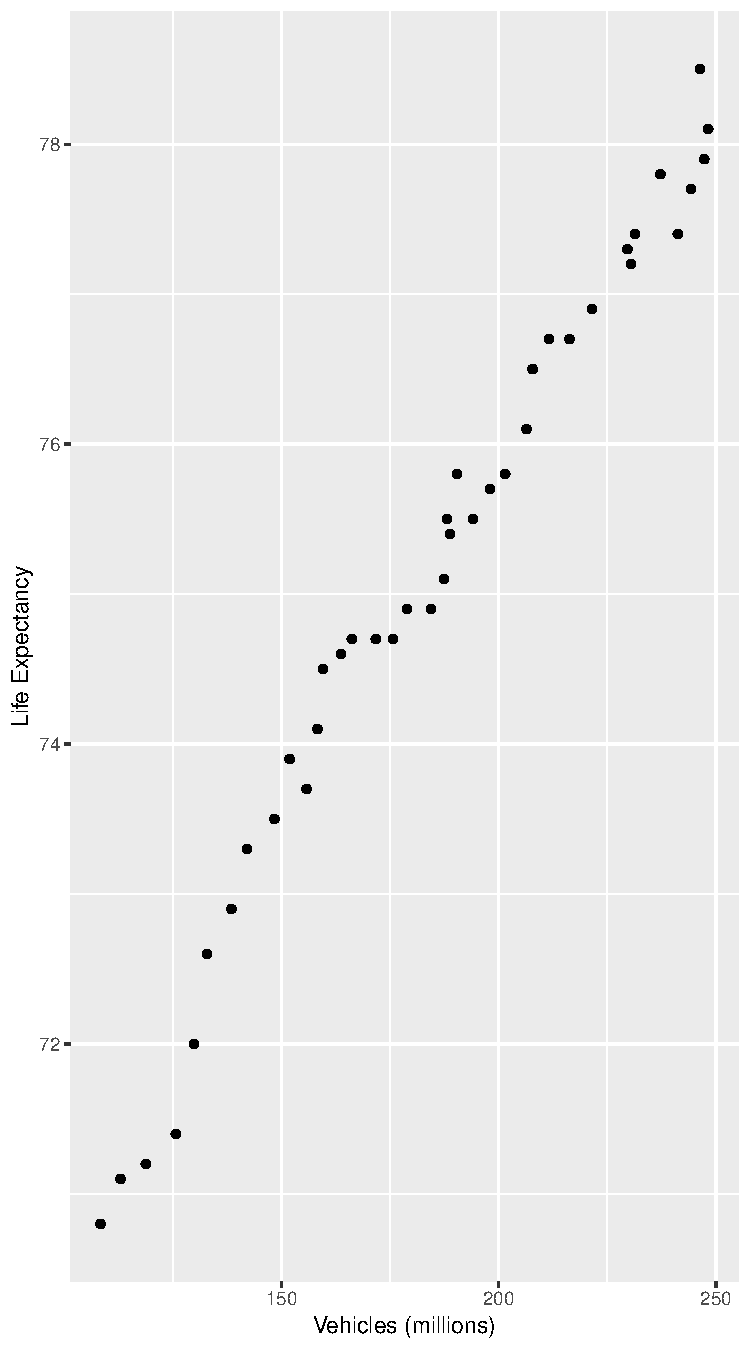
\includegraphics[width=0.65\linewidth]{Lock5WithR_files/figure-latex/Figure1.2-1}

\hypertarget{observational-studies-vs.-experiments}{%
\subsection{Observational Studies vs.~Experiments}\label{observational-studies-vs.-experiments}}

Statisticians use the word experiment to mean something very specific. \emph{In an \textbf{experiment}, the researcher determines the values of one or more (explanatory) variables}, typically by random assignment. If there is no such assignment by the researcher, the study is an \textbf{observational study}.

\hypertarget{describing-data}{%
\chapter{Describing Data}\label{describing-data}}

In this chapter we discuss graphical and numerical summaries of data.

\hypertarget{categorical-variables}{%
\section{Categorical Variables}\label{categorical-variables}}

Let us investigate categorical variables in R by taking a look at the data set for the One True Love survey. Notice that the data set is not readily available in our textbook's package. However, the authors do provide us with the necessary information to create our own data spreadsheet (in either Excel or Google) and import it into R (See Chapter 0 for instructions.)

\begin{Shaded}
\begin{Highlighting}[]
\NormalTok{OneTrueLove <-}\StringTok{ }\KeywordTok{read.file}\NormalTok{( }\StringTok{"OneTrueLove.csv"}\NormalTok{ )}
\end{Highlighting}
\end{Shaded}

\begin{verbatim}
## Reading data with read.csv()
\end{verbatim}

Alternatively, we can read from a URL like this

\begin{Shaded}
\begin{Highlighting}[]
\NormalTok{OneTrueLove2 <-}\StringTok{ }
\StringTok{  }\KeywordTok{read.file}\NormalTok{(}\StringTok{"https://raw.githubusercontent.com/rpruim/Lock5withR/master/Book/OneTrueLove.csv"}\NormalTok{)}
\end{Highlighting}
\end{Shaded}

\hypertarget{one-categorical-variable}{%
\subsection{One Categorical Variable}\label{one-categorical-variable}}

From the dataset we named as {OneTrueLove}, we can use the \texttt{prop()()} function to quickly find \textbf{proportions}.

\begin{Shaded}
\begin{Highlighting}[]
\KeywordTok{prop}\NormalTok{( }\OperatorTok{~}\StringTok{ }\NormalTok{Response, }\DataTypeTok{data =}\NormalTok{ OneTrueLove)}
\end{Highlighting}
\end{Shaded}

\begin{verbatim}
## prop_Agree 
##       0.28
\end{verbatim}

\hypertarget{table-2.1}{%
\subsubsection{Table 2.1}\label{table-2.1}}

We can also tabulate the categorical variable to display the \emph{frequency} by using the \texttt{tally()()} function. The default in tallying is to not include the row totals, or column totals when there are two variables. These are called marginal totals and if you want them, you can change the default.

\begin{Shaded}
\begin{Highlighting}[]
\KeywordTok{tally}\NormalTok{( }\OperatorTok{~}\StringTok{ }\NormalTok{Response, }\DataTypeTok{margin =} \OtherTok{TRUE}\NormalTok{, }\DataTypeTok{data =}\NormalTok{ OneTrueLove)}
\end{Highlighting}
\end{Shaded}

\begin{verbatim}
## Response
##      Agree   Disagree Don't know      Total 
##        735       1812         78       2625
\end{verbatim}

\hypertarget{example-2.3}{%
\subsubsection{Example 2.3}\label{example-2.3}}

To find the proportion of responders who \emph{disagree} or \emph{don't know}, we can use the {level=} argument in the function to find proportions.

\begin{Shaded}
\begin{Highlighting}[]
\KeywordTok{prop}\NormalTok{( }\OperatorTok{~}\StringTok{ }\NormalTok{Response, }\DataTypeTok{success =} \StringTok{"Disagree"}\NormalTok{, }\DataTypeTok{data =}\NormalTok{ OneTrueLove)}
\end{Highlighting}
\end{Shaded}

\begin{verbatim}
## prop_Disagree 
##     0.6902857
\end{verbatim}

\begin{Shaded}
\begin{Highlighting}[]
\KeywordTok{prop}\NormalTok{( }\OperatorTok{~}\StringTok{ }\NormalTok{Response, }\DataTypeTok{success =} \StringTok{"Don't know"}\NormalTok{, }\DataTypeTok{data =}\NormalTok{ OneTrueLove)}
\end{Highlighting}
\end{Shaded}

\begin{verbatim}
## prop_Don't know 
##      0.02971429
\end{verbatim}

Further, we can also display the \emph{relative frequencies}, or \textbf{proportions} in a table.

\begin{Shaded}
\begin{Highlighting}[]
\KeywordTok{tally}\NormalTok{( }\OperatorTok{~}\StringTok{ }\NormalTok{Response, }\DataTypeTok{format =} \StringTok{"proportion"}\NormalTok{, }\DataTypeTok{margin =} \OtherTok{TRUE}\NormalTok{, }\DataTypeTok{data =}\NormalTok{ OneTrueLove)}
\end{Highlighting}
\end{Shaded}

\begin{verbatim}
## Response
##      Agree   Disagree Don't know      Total 
## 0.28000000 0.69028571 0.02971429 1.00000000
\end{verbatim}

\hypertarget{figure-2.1}{%
\subsubsection{Figure 2.1}\label{figure-2.1}}

R provides many different chart and plot functions, including \emph{bar charts} and \emph{pie charts}, to visualize counts or proportions. Bar charts, also known as bar graphs, are a way of displaying the distribution of a categorical variable.

\begin{Shaded}
\begin{Highlighting}[]
\KeywordTok{gf_bar}\NormalTok{( }\OperatorTok{~}\StringTok{ }\NormalTok{Response, }\DataTypeTok{data =}\NormalTok{ OneTrueLove)}
\end{Highlighting}
\end{Shaded}

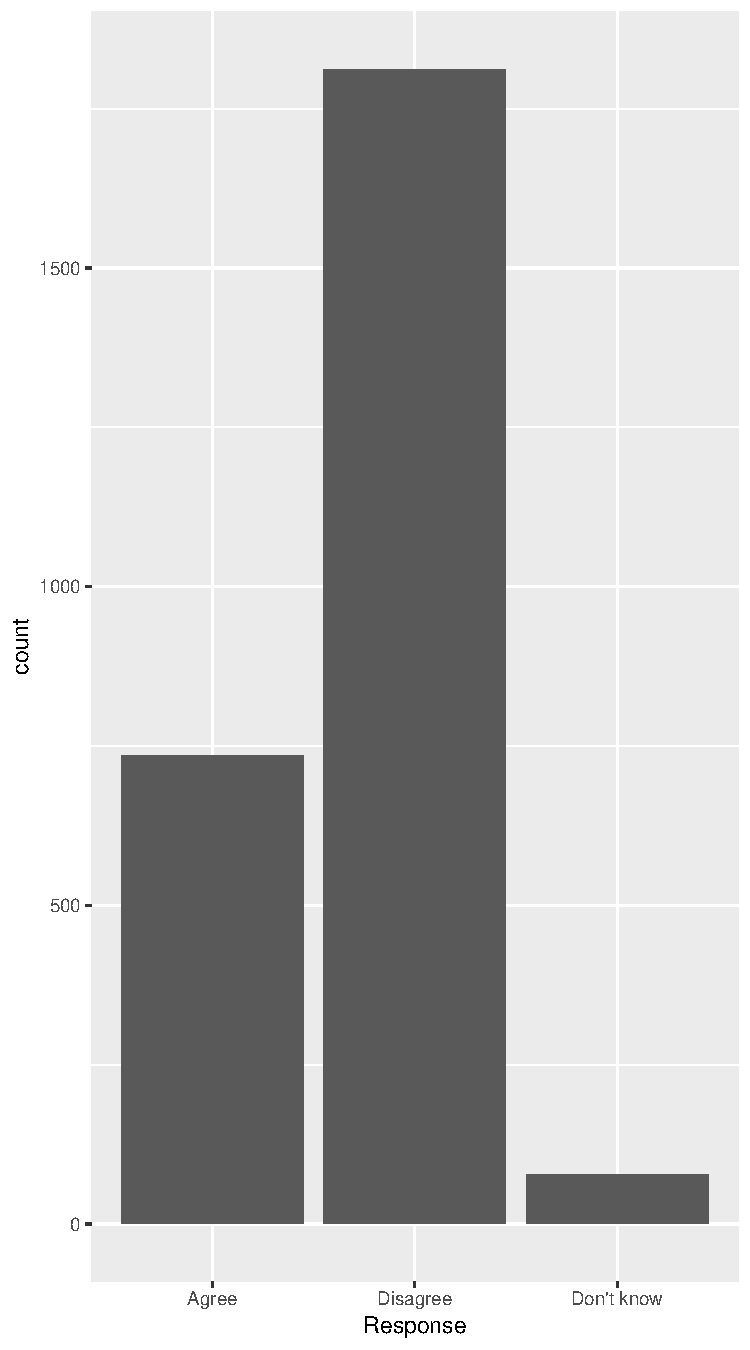
\includegraphics[width=0.65\linewidth]{Lock5WithR_files/figure-latex/Figure2.1-1}

\hypertarget{two-categorical-variables-two-way-tables}{%
\subsection{Two Categorical Variables: Two-Way Tables}\label{two-categorical-variables-two-way-tables}}

Often, it is useful to compute cross tables for two (or more) variables. We can again use \texttt{tally()()} for several ways to investigate a two-way table.

\hypertarget{table-2.3}{%
\subsubsection{Table 2.3}\label{table-2.3}}

\begin{Shaded}
\begin{Highlighting}[]
\KeywordTok{tally}\NormalTok{( }\OperatorTok{~}\StringTok{ }\NormalTok{Response }\OperatorTok{+}\StringTok{ }\NormalTok{Gender, }\DataTypeTok{data =}\NormalTok{ OneTrueLove)}
\end{Highlighting}
\end{Shaded}

\begin{verbatim}
##             Gender
## Response     Female Male
##   Agree         363  372
##   Disagree     1005  807
##   Don't know     44   34
\end{verbatim}

\hypertarget{table-2.4}{%
\subsubsection{Table 2.4}\label{table-2.4}}

\begin{Shaded}
\begin{Highlighting}[]
\KeywordTok{tally}\NormalTok{( }\OperatorTok{~}\StringTok{ }\NormalTok{Response }\OperatorTok{+}\StringTok{ }\NormalTok{Gender, }\DataTypeTok{margins =} \OtherTok{TRUE}\NormalTok{, }\DataTypeTok{data =}\NormalTok{ OneTrueLove)}
\end{Highlighting}
\end{Shaded}

\begin{verbatim}
##             Gender
## Response     Female Male Total
##   Agree         363  372   735
##   Disagree     1005  807  1812
##   Don't know     44   34    78
##   Total        1412 1213  2625
\end{verbatim}

\hypertarget{example-2.5}{%
\subsubsection{Example 2.5}\label{example-2.5}}

Similar to one categorical variable, we can use the \texttt{prop()()} function to find the proportion of two variables. The first line results in the proportion of females who agree and the proportion of males who agree. The second line shows the proportion who agree that are female and the proportion who disagree that are female. The third results in the proportion of all the survey responders that are female.

\begin{Shaded}
\begin{Highlighting}[]
\KeywordTok{prop}\NormalTok{(Response}\OperatorTok{~}\NormalTok{Gender, }\DataTypeTok{data =}\NormalTok{ OneTrueLove)}
\end{Highlighting}
\end{Shaded}

\begin{verbatim}
## prop_Agree.Female   prop_Agree.Male 
##         0.2570822         0.3066777
\end{verbatim}

\begin{Shaded}
\begin{Highlighting}[]
\KeywordTok{prop}\NormalTok{(Gender}\OperatorTok{~}\NormalTok{Response, }\DataTypeTok{data =}\NormalTok{ OneTrueLove)}
\end{Highlighting}
\end{Shaded}

\begin{verbatim}
##      prop_Female.Agree   prop_Female.Disagree prop_Female.Don't know 
##              0.4938776              0.5546358              0.5641026
\end{verbatim}

\begin{Shaded}
\begin{Highlighting}[]
\KeywordTok{prop}\NormalTok{( }\OperatorTok{~}\StringTok{ }\NormalTok{Gender, }\DataTypeTok{data =}\NormalTok{ OneTrueLove)}
\end{Highlighting}
\end{Shaded}

\begin{verbatim}
## prop_Female 
##   0.5379048
\end{verbatim}

See though that because we have multiple levels of each variable, this process can become quite tedious if we want to find the proportions for all of the levels. Using the tally function a little differently will result in these proportions.

\begin{Shaded}
\begin{Highlighting}[]
\KeywordTok{tally}\NormalTok{(Response }\OperatorTok{~}\StringTok{ }\NormalTok{Gender, }\DataTypeTok{data =}\NormalTok{ OneTrueLove)}
\end{Highlighting}
\end{Shaded}

\begin{verbatim}
##             Gender
## Response     Female Male
##   Agree         363  372
##   Disagree     1005  807
##   Don't know     44   34
\end{verbatim}

\begin{Shaded}
\begin{Highlighting}[]
\KeywordTok{tally}\NormalTok{( }\OperatorTok{~}\StringTok{ }\NormalTok{Response }\OperatorTok{|}\StringTok{ }\NormalTok{Gender, }\DataTypeTok{data =}\NormalTok{ OneTrueLove)}
\end{Highlighting}
\end{Shaded}

\begin{verbatim}
##             Gender
## Response     Female Male
##   Agree         363  372
##   Disagree     1005  807
##   Don't know     44   34
\end{verbatim}

\begin{Shaded}
\begin{Highlighting}[]
\KeywordTok{tally}\NormalTok{(Gender }\OperatorTok{~}\StringTok{ }\NormalTok{Response, }\DataTypeTok{data =}\NormalTok{ OneTrueLove)}
\end{Highlighting}
\end{Shaded}

\begin{verbatim}
##         Response
## Gender   Agree Disagree Don't know
##   Female   363     1005         44
##   Male     372      807         34
\end{verbatim}

\begin{Shaded}
\begin{Highlighting}[]
\KeywordTok{tally}\NormalTok{( }\OperatorTok{~}\StringTok{ }\NormalTok{Gender }\OperatorTok{|}\StringTok{ }\NormalTok{Response, }\DataTypeTok{data =}\NormalTok{ OneTrueLove)}
\end{Highlighting}
\end{Shaded}

\begin{verbatim}
##         Response
## Gender   Agree Disagree Don't know
##   Female   363     1005         44
##   Male     372      807         34
\end{verbatim}

Notice that (by default) some of these use counts and some use proportions. Again, we can change the format.

\begin{Shaded}
\begin{Highlighting}[]
\KeywordTok{tally}\NormalTok{( }\OperatorTok{~}\StringTok{ }\NormalTok{Gender, }\DataTypeTok{format =} \StringTok{"percent"}\NormalTok{, }\DataTypeTok{data =}\NormalTok{ OneTrueLove)}
\end{Highlighting}
\end{Shaded}

\begin{verbatim}
## Gender
##   Female     Male 
## 53.79048 46.20952
\end{verbatim}

\hypertarget{example-2.6}{%
\subsubsection{Example 2.6}\label{example-2.6}}

\begin{Shaded}
\begin{Highlighting}[]
\KeywordTok{tally}\NormalTok{( }\OperatorTok{~}\StringTok{ }\NormalTok{Gender }\OperatorTok{+}\StringTok{ }\NormalTok{Award, }\DataTypeTok{margin =} \OtherTok{TRUE}\NormalTok{, }\DataTypeTok{data =}\NormalTok{ StudentSurvey)}
\end{Highlighting}
\end{Shaded}

\begin{verbatim}
##        Award
## Gender  Academy Nobel Olympic Total
##   F          20    76      73   169
##   M          11    73     109   193
##   Total      31   149     182   362
\end{verbatim}

Also, we can arrange the table differently by converting it to a data frame.

\begin{Shaded}
\begin{Highlighting}[]
\KeywordTok{as.data.frame}\NormalTok{(}\KeywordTok{tally}\NormalTok{( }\OperatorTok{~}\StringTok{ }\NormalTok{Gender }\OperatorTok{+}\StringTok{ }\NormalTok{Award, }\DataTypeTok{data =}\NormalTok{ StudentSurvey))}
\end{Highlighting}
\end{Shaded}

\begin{verbatim}
##   Gender   Award Freq
## 1      F Academy   20
## 2      M Academy   11
## 3      F   Nobel   76
## 4      M   Nobel   73
## 5      F Olympic   73
## 6      M Olympic  109
\end{verbatim}

\begin{Shaded}
\begin{Highlighting}[]
\KeywordTok{prop}\NormalTok{( }\OperatorTok{~}\StringTok{ }\NormalTok{Award, }\DataTypeTok{success =} \StringTok{"Olympic"}\NormalTok{, }\DataTypeTok{data =}\NormalTok{ StudentSurvey)}
\end{Highlighting}
\end{Shaded}

\begin{verbatim}
## prop_Olympic 
##    0.5027624
\end{verbatim}

\hypertarget{example-2.7}{%
\subsubsection{Example 2.7}\label{example-2.7}}

To calculate the difference of certain statistics, we can use the \texttt{diff()()} function. Here we use it to find the difference in proportions, but it can be used for means, medians, and etc.

\begin{Shaded}
\begin{Highlighting}[]
\KeywordTok{diff}\NormalTok{(}\KeywordTok{prop}\NormalTok{(Award}\OperatorTok{~}\NormalTok{Gender, }\DataTypeTok{success =} \StringTok{"Olympic"}\NormalTok{, }\DataTypeTok{data =}\NormalTok{ StudentSurvey))}
\end{Highlighting}
\end{Shaded}

\begin{verbatim}
## prop_Olympic.M 
##      0.1328142
\end{verbatim}

We will continue more with proportions in Chapter 3.

\hypertarget{figure-2.2}{%
\subsubsection{Figure 2.2}\label{figure-2.2}}

A way to look at multiple groups simultaneously is by using \emph{comparative plots} such as a \emph{segmented bar chart} or \emph{side-by-side bar chart}. We often use the {fill} argument for this. {fill} is used when the assigned data is represented as an area, rather than a line or point.
\footnote{For coloring a line or point, \texttt{colour()} is used}

Notice the addition of {fill=} (to group) and {position=} (to segment the graph). The default of {position=} is to stack the bar graph, so for the first example we can disclude the argument.
TEX COMMAND NOT FOUND authNote Rewrote paragraph and footnote

\begin{Shaded}
\begin{Highlighting}[]
\KeywordTok{gf_bar}\NormalTok{( }\OperatorTok{~}\StringTok{ }\NormalTok{Award, }\DataTypeTok{fill =} \OperatorTok{~}\NormalTok{Gender, }\DataTypeTok{data =}\NormalTok{ StudentSurvey)}
\end{Highlighting}
\end{Shaded}

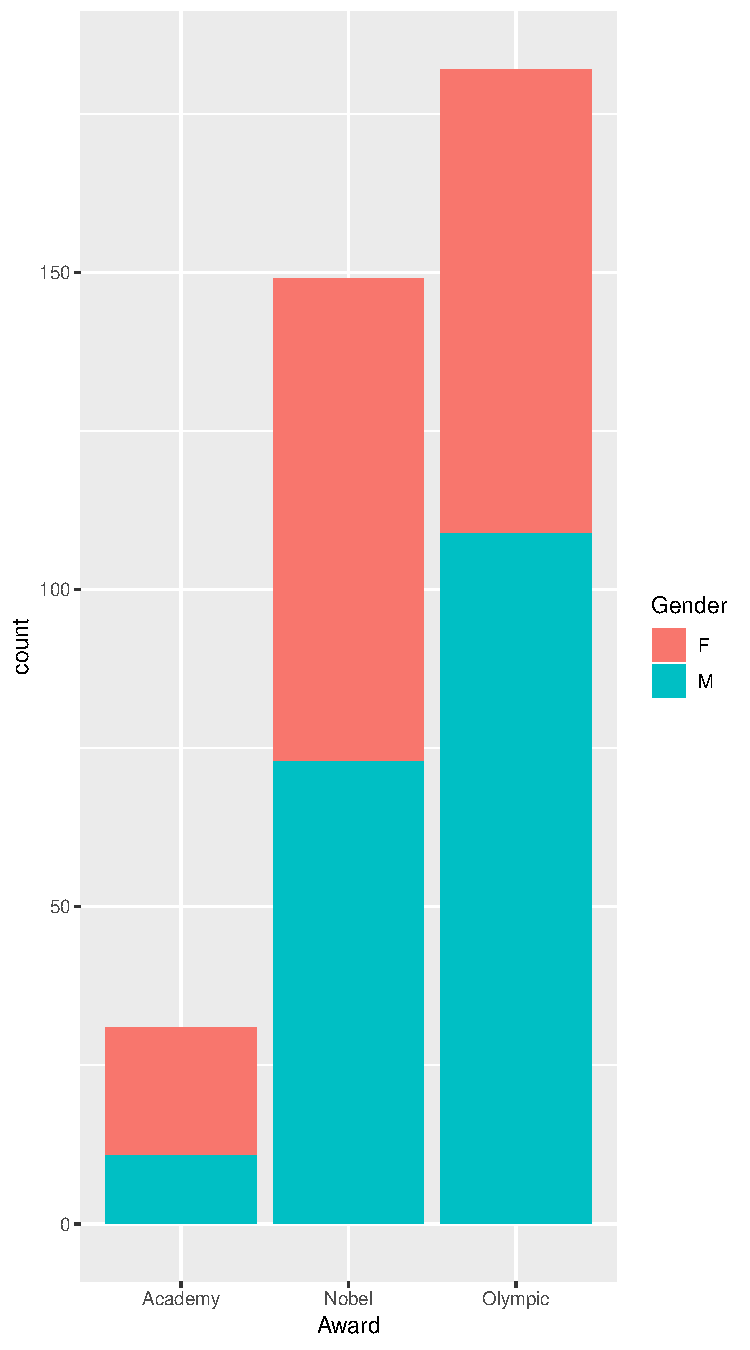
\includegraphics[width=0.65\linewidth]{Lock5WithR_files/figure-latex/Figure2.2-1}

\begin{Shaded}
\begin{Highlighting}[]
\KeywordTok{gf_bar}\NormalTok{( }\OperatorTok{~}\StringTok{ }\NormalTok{Gender, }\DataTypeTok{fill =} \OperatorTok{~}\NormalTok{Award, }\DataTypeTok{position =} \StringTok{'dodge'}\NormalTok{, }\DataTypeTok{data =}\NormalTok{ StudentSurvey)}
\end{Highlighting}
\end{Shaded}

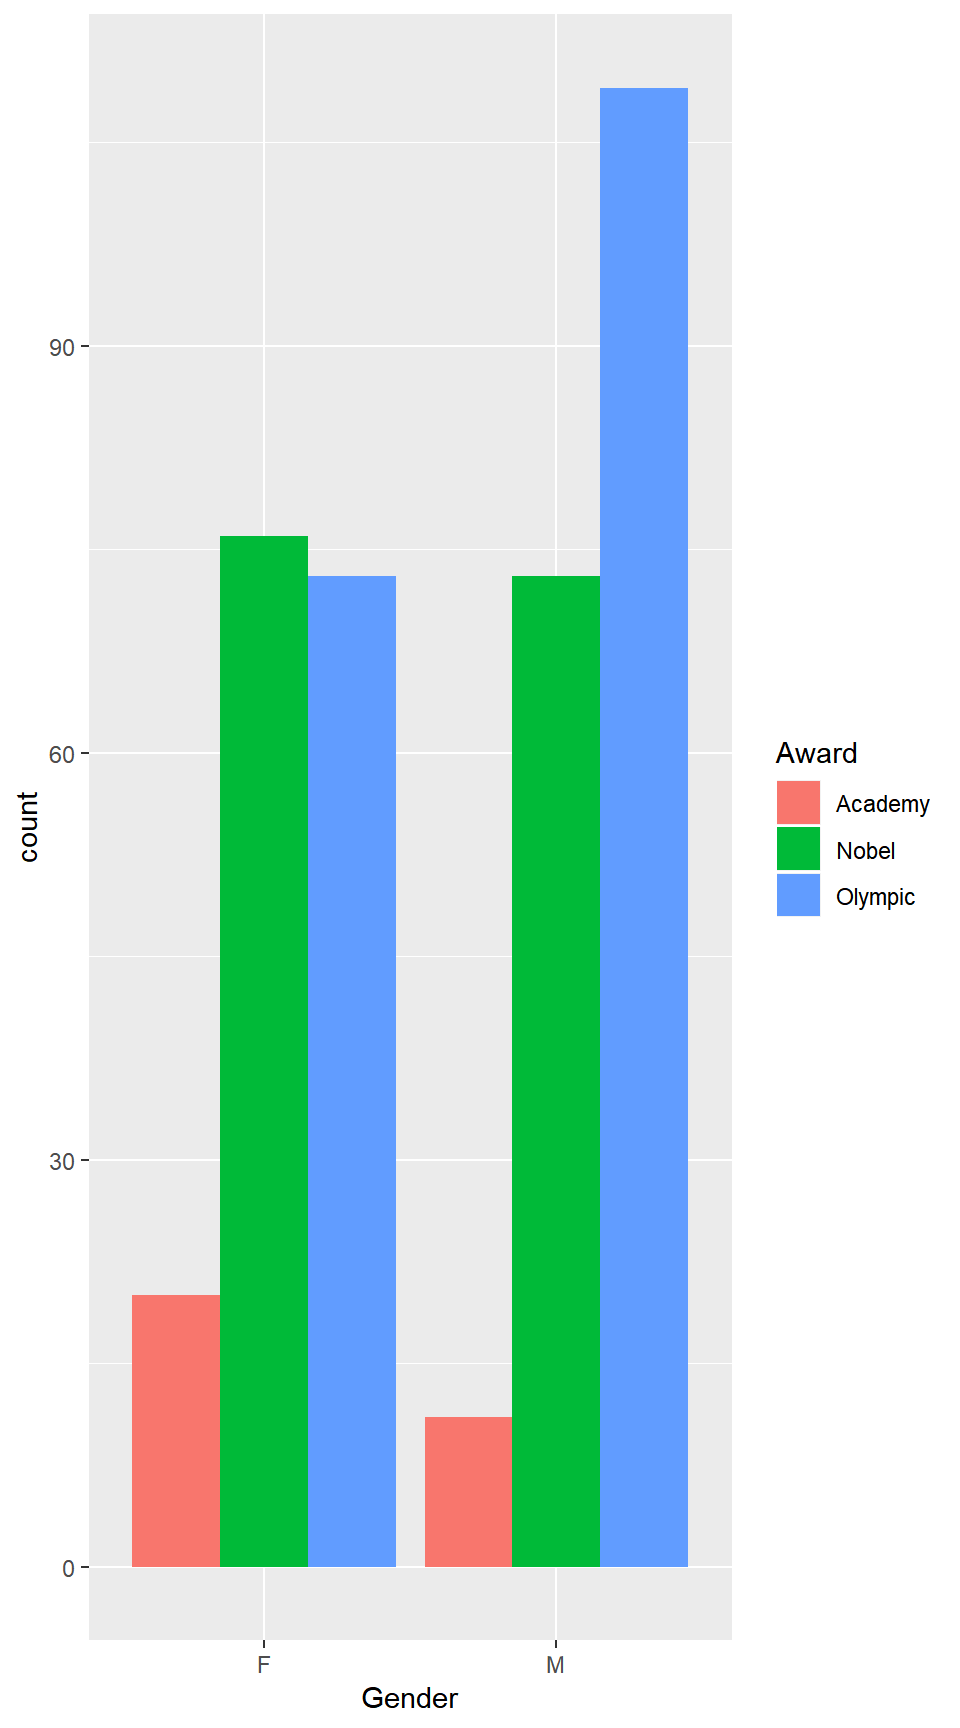
\includegraphics[width=0.65\linewidth]{Lock5WithR_files/figure-latex/Figure2.2b-1}

\hypertarget{one-quantitative-variable-shape-and-center}{%
\section{One Quantitative Variable: Shape and Center}\label{one-quantitative-variable-shape-and-center}}

\begin{center}\rule{0.5\linewidth}{\linethickness}\end{center}

The distribution of a variable answers two questions:

\begin{enumerate}
\tightlist
\item
  \emph{What values} can the variable have?
\item
  \emph{With what frequency} does each value occur?
\end{enumerate}

Again, the frequency may be described in terms of counts, proportions (often called
relative frequency), or densities (more on densities later).

\begin{center}\rule{0.5\linewidth}{\linethickness}\end{center}

A distribution may be described using a table (listing values and frequencies)
or a graph (e.g., a histogram) or with words that describe general features
of the distribution (e.g., symmetric, skewed).

\hypertarget{the-shape-of-a-distribution}{%
\subsection{The Shape of a Distribution}\label{the-shape-of-a-distribution}}

\hypertarget{table-2.14}{%
\subsubsection{Table 2.14}\label{table-2.14}}

\begin{Shaded}
\begin{Highlighting}[]
\NormalTok{MammalLongevity}
\end{Highlighting}
\end{Shaded}

\begin{verbatim}
##          Animal Gestation Longevity
## 1        baboon       187        20
## 2    bear,black       219        18
## 3  bear,grizzly       225        25
## 4    bear,polar       240        20
## 5        beaver       122         5
## 6       buffalo       278        15
## 7         camel       406        12
## 8           cat        63        12
## 9    chimpanzee       231        20
## 10     chipmunk        31         6
## 11          cow       284        15
## 12         deer       201         8
## 13          dog        61        12
## 14       donkey       365        12
## 15     elephant       645        40
## 16          elk       250        15
## 17          fox        52         7
## 18      giraffe       425        10
## 19         goat       151         8
## 20      gorilla       257        20
## 21   guinea pig        68         4
## 22 hippopotamus       238        25
## 23        horse       330        20
## 24     kangaroo        42         7
## 25      leopard        98        12
## 26         lion       100        15
## 27       monkey       164        15
## 28        moose       240        12
## 29        mouse        21         3
## 30      opposum        15         1
## 31          pig       112        10
## 32         puma        90        12
## 33       rabbit        31         5
## 34   rhinoceros       450        15
## 35     sea lion       350        12
## 36        sheep       154        12
## 37     squirrel        44        10
## 38        tiger       105        16
## 39         wolf        63         5
## 40        zebra       365        15
\end{verbatim}

Statisticians have devised a number of graphs to help us see distributions visually.\\
The general syntax for making a graph of one variable in a data frame is

\begin{Shaded}
\begin{Highlighting}[]
\KeywordTok{plotname}\NormalTok{( }\OperatorTok{~}\StringTok{ }\NormalTok{variable, }\DataTypeTok{data =}\NormalTok{ dataName)}
\end{Highlighting}
\end{Shaded}

In other words, there are three pieces of information we must provide to
R in order to get the plot we want:

\begin{enumerate}
\item
\begin{verbatim}
   The kind of plot (`gf_histogram()()`, `gf_bar()()`, 
\end{verbatim}

  \texttt{gf\_dens()()}, etc.)
  \#. The name of the variable
  \#. The name of the data frame this variable is a part of.
\end{enumerate}

This should look familiar from the previous section.

\hypertarget{figure-2.6}{%
\subsubsection{Figure 2.6}\label{figure-2.6}}

Let's make a \emph{dot plot} of the variable Longevity in the {MammalLongevity} data set for a quick and simple look at the distribution. We use the syntax provided above with two additional arguments to make the figure look the way we want it to. The next few sections will explain a few of the different arguments available for plots in R

\begin{Shaded}
\begin{Highlighting}[]
\KeywordTok{gf_dotplot}\NormalTok{(}\OperatorTok{~}\StringTok{ }\NormalTok{Longevity, }\DataTypeTok{binwidth =} \DecValTok{1}\NormalTok{, }\DataTypeTok{dotsize =} \FloatTok{.75}\NormalTok{, }\DataTypeTok{data =}\NormalTok{ MammalLongevity)}
\end{Highlighting}
\end{Shaded}

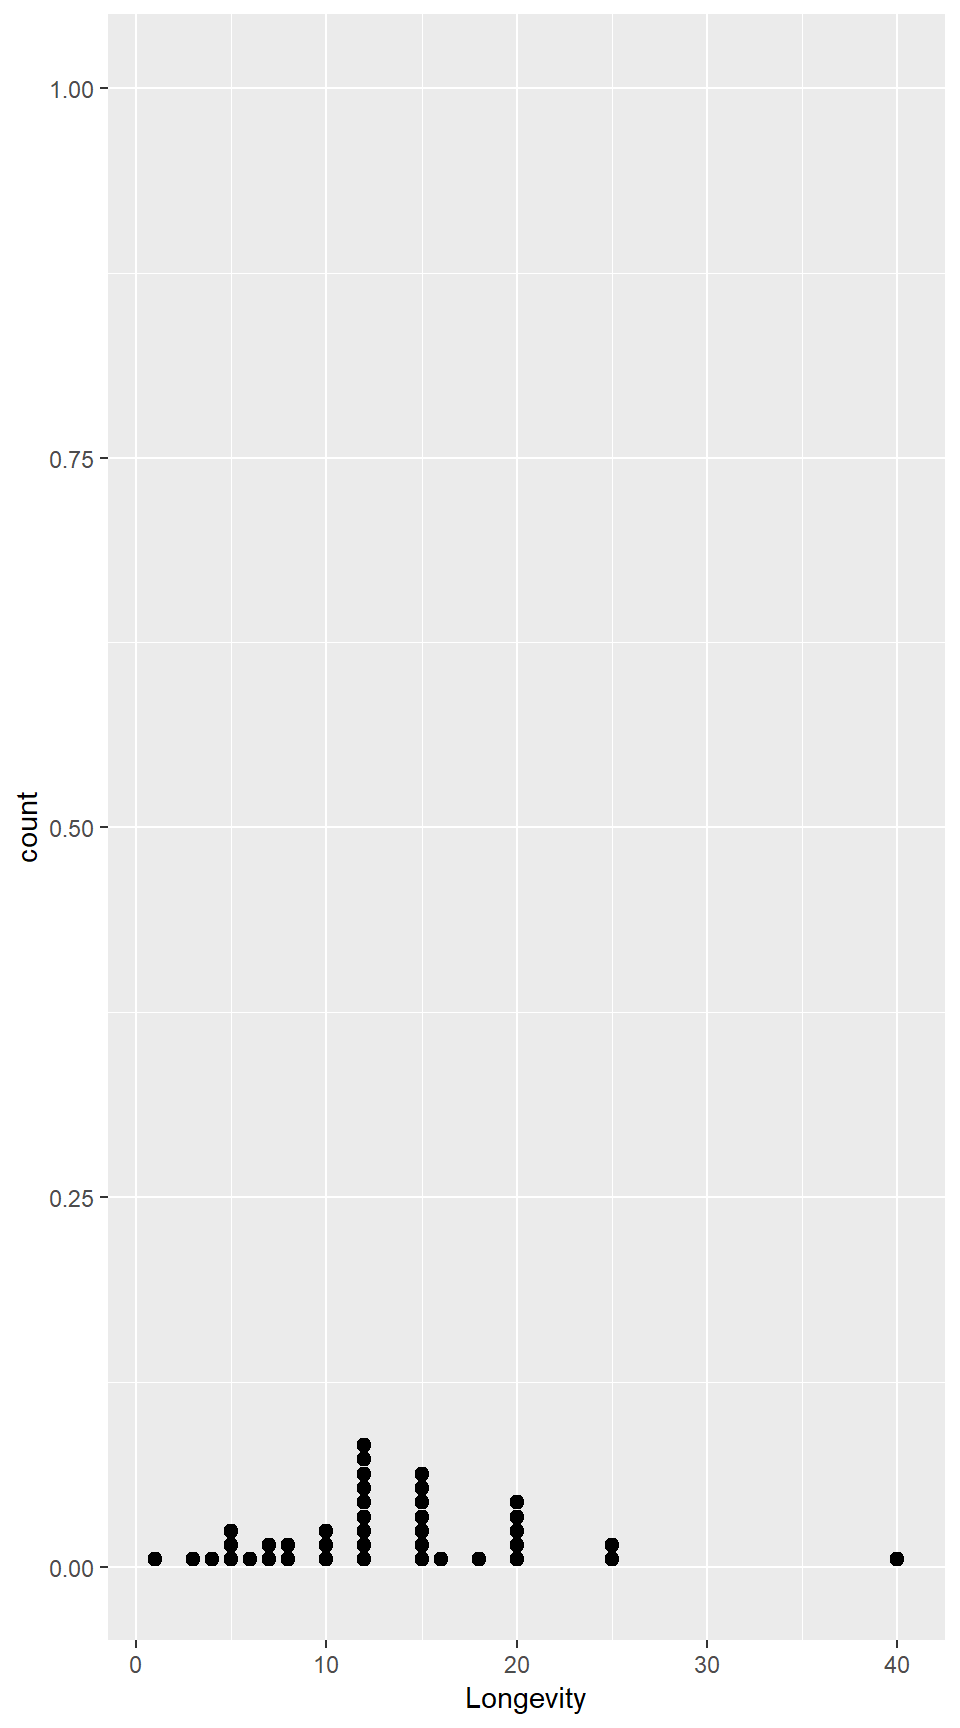
\includegraphics[width=0.65\linewidth]{Lock5WithR_files/figure-latex/Figure2.6-1}

\hypertarget{table-2.15}{%
\subsubsection{Table 2.15}\label{table-2.15}}

Although \texttt{tally()()} works with quantitative variables as well as categorical variables, this is only useful when there are not too many different values for the variable.

\begin{Shaded}
\begin{Highlighting}[]
\KeywordTok{tally}\NormalTok{( }\OperatorTok{~}\StringTok{ }\NormalTok{Longevity, }\DataTypeTok{margin =} \OtherTok{TRUE}\NormalTok{, }\DataTypeTok{data =}\NormalTok{ MammalLongevity)}
\end{Highlighting}
\end{Shaded}

\begin{verbatim}
## Longevity
##     1     3     4     5     6     7     8    10    12    15    16    18 
##     1     1     1     3     1     2     2     3     9     7     1     1 
##    20    25    40 Total 
##     5     2     1    40
\end{verbatim}

Sometimes, it is more convenient to group them into bins. We just have to tell R what the bins are. For example, suppose we wanted to group together by 5.
cut()
tally()

\begin{Shaded}
\begin{Highlighting}[]
\NormalTok{binned.long <-}\StringTok{ }\KeywordTok{cut}\NormalTok{(MammalLongevity}\OperatorTok{$}\NormalTok{Longevity, }\DataTypeTok{breaks =} \KeywordTok{c}\NormalTok{(}\DecValTok{0}\NormalTok{,}\DecValTok{5}\NormalTok{,}\DecValTok{10}\NormalTok{,}\DecValTok{15}\NormalTok{,}\DecValTok{20}\NormalTok{,}\DecValTok{25}\NormalTok{,}\DecValTok{30}\NormalTok{,}\DecValTok{35}\NormalTok{,}\DecValTok{40}\NormalTok{))}
\KeywordTok{tally}\NormalTok{( }\OperatorTok{~}\StringTok{ }\NormalTok{binned.long)      }\CommentTok{# no data frame given because it is not in a data frame}
\end{Highlighting}
\end{Shaded}

\begin{verbatim}
## binned.long
##   (0,5]  (5,10] (10,15] (15,20] (20,25] (25,30] (30,35] (35,40] 
##       6       8      16       7       2       0       0       1
\end{verbatim}

Suppose we wanted to group the 1s, 10s, 20s, etc. together. We want to make sure then that 10 is with the 10s, so we should add another argument.
\textless\textless Table2.15c\textgreater\textgreater=
binned.long2 \textless- cut(MammalLongevity\$Longevity, breaks = c(0,10,20,30,40,50), right = FALSE)
tally( \textasciitilde{} binned.long2) \# no data frame given because it is not in a data frame
@

We won't use this very often however, since seeing this information in a histogram is typically more useful.

\hypertarget{figure-2.7}{%
\subsubsection{Figure 2.7}\label{figure-2.7}}

Histograms are a way of displaying the distribution of a quantitative variable.
\textless\textless Figure2.7\textgreater\textgreater=
gf\_histogram( \textasciitilde{} Longevity, binwidth = 5, data = MammalLongevity)
@

We can control the (approximate) number of bins using the {bins} argument. The number of bins (and to a lesser extent the positions of the bins) can make a histogram look quite different.

\begin{Shaded}
\begin{Highlighting}[]
\KeywordTok{gf_histogram}\NormalTok{( }\OperatorTok{~}\StringTok{ }\NormalTok{Longevity, }\DataTypeTok{data =}\NormalTok{ MammalLongevity, }\DataTypeTok{bins =} \DecValTok{8}\NormalTok{)}
\end{Highlighting}
\end{Shaded}

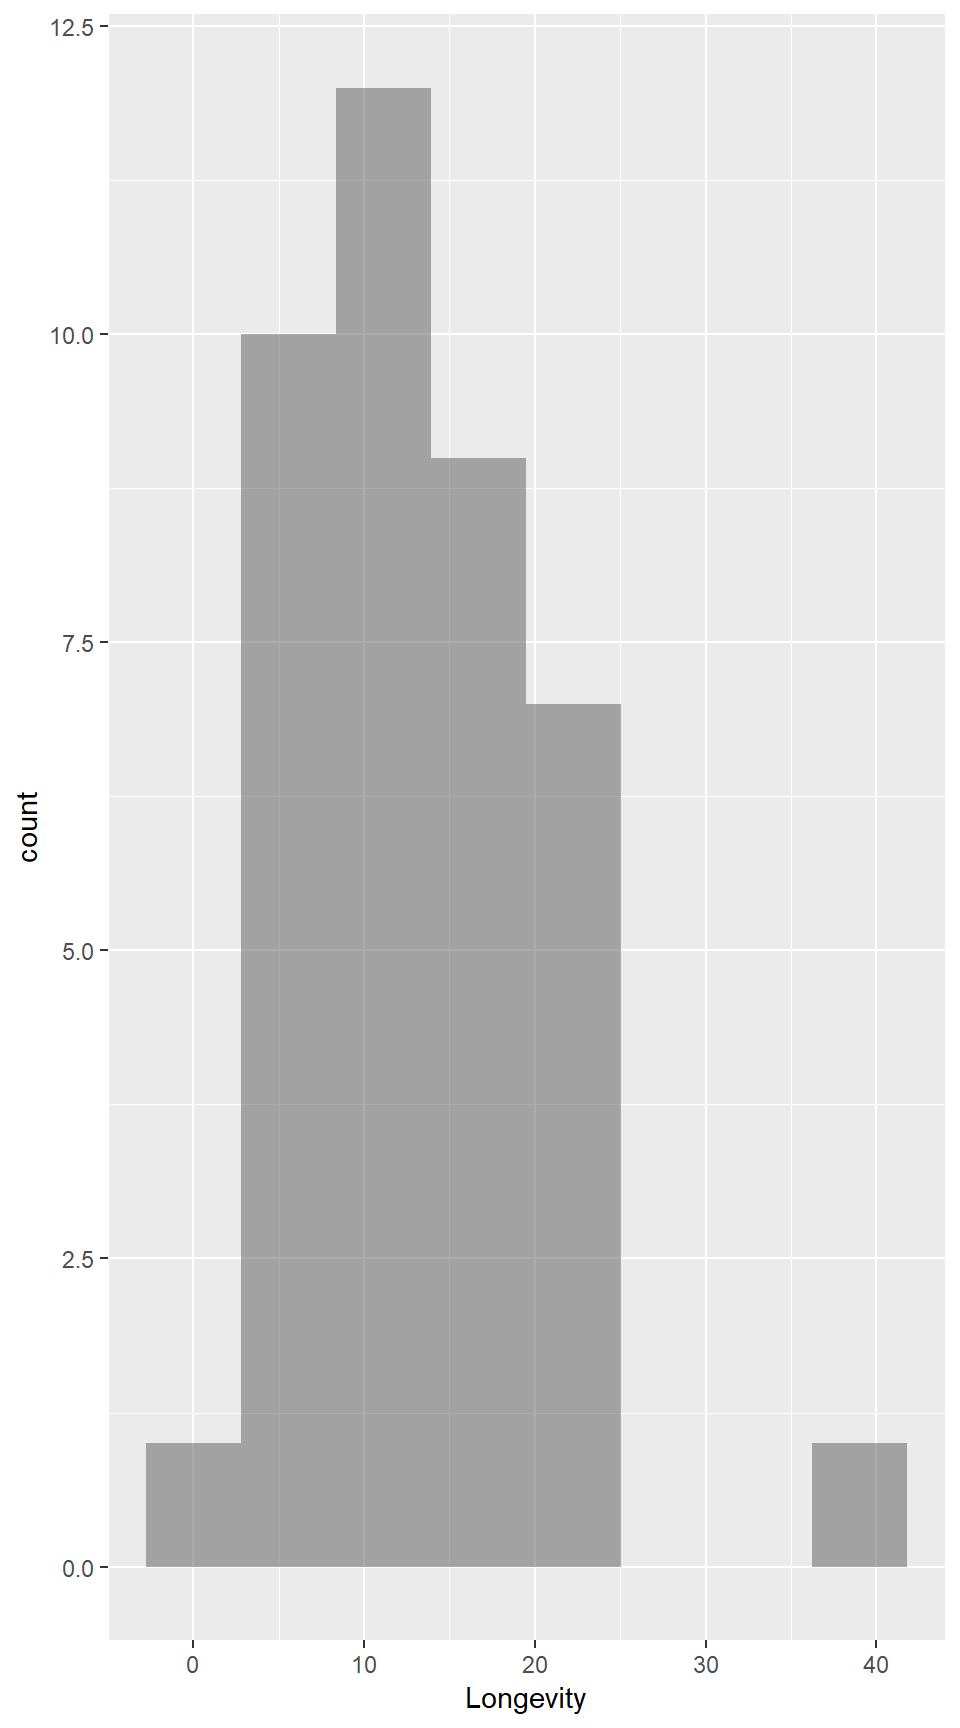
\includegraphics[width=0.65\linewidth]{Lock5WithR_files/figure-latex/Figure2.7b-1}

\begin{Shaded}
\begin{Highlighting}[]
\KeywordTok{gf_histogram}\NormalTok{( }\OperatorTok{~}\StringTok{ }\NormalTok{Longevity, }\DataTypeTok{data =}\NormalTok{ MammalLongevity, }\DataTypeTok{bins =} \DecValTok{15}\NormalTok{)}
\end{Highlighting}
\end{Shaded}

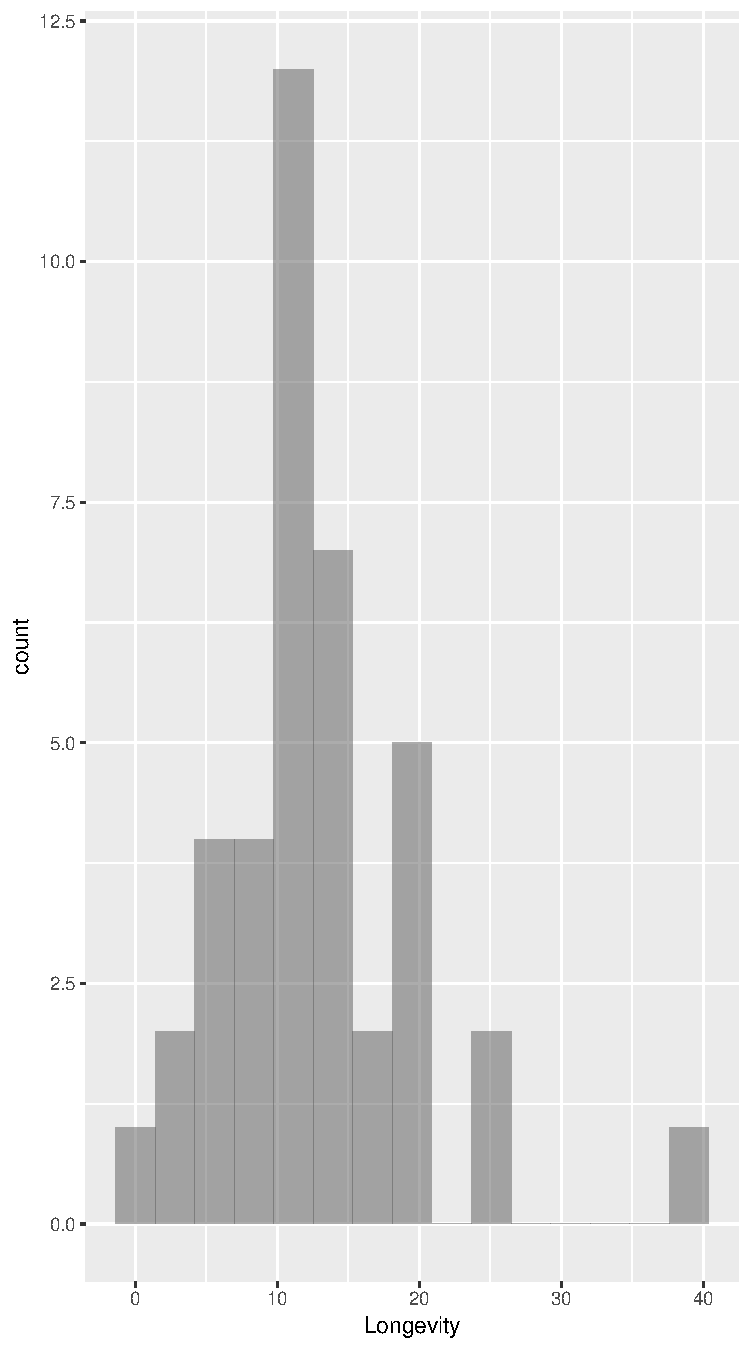
\includegraphics[width=0.65\linewidth]{Lock5WithR_files/figure-latex/Figure2.7b-2}

\begin{Shaded}
\begin{Highlighting}[]
\KeywordTok{gf_histogram}\NormalTok{( }\OperatorTok{~}\StringTok{ }\NormalTok{Longevity, }\DataTypeTok{data =}\NormalTok{ MammalLongevity, }\DataTypeTok{bins =} \DecValTok{30}\NormalTok{)}
\end{Highlighting}
\end{Shaded}

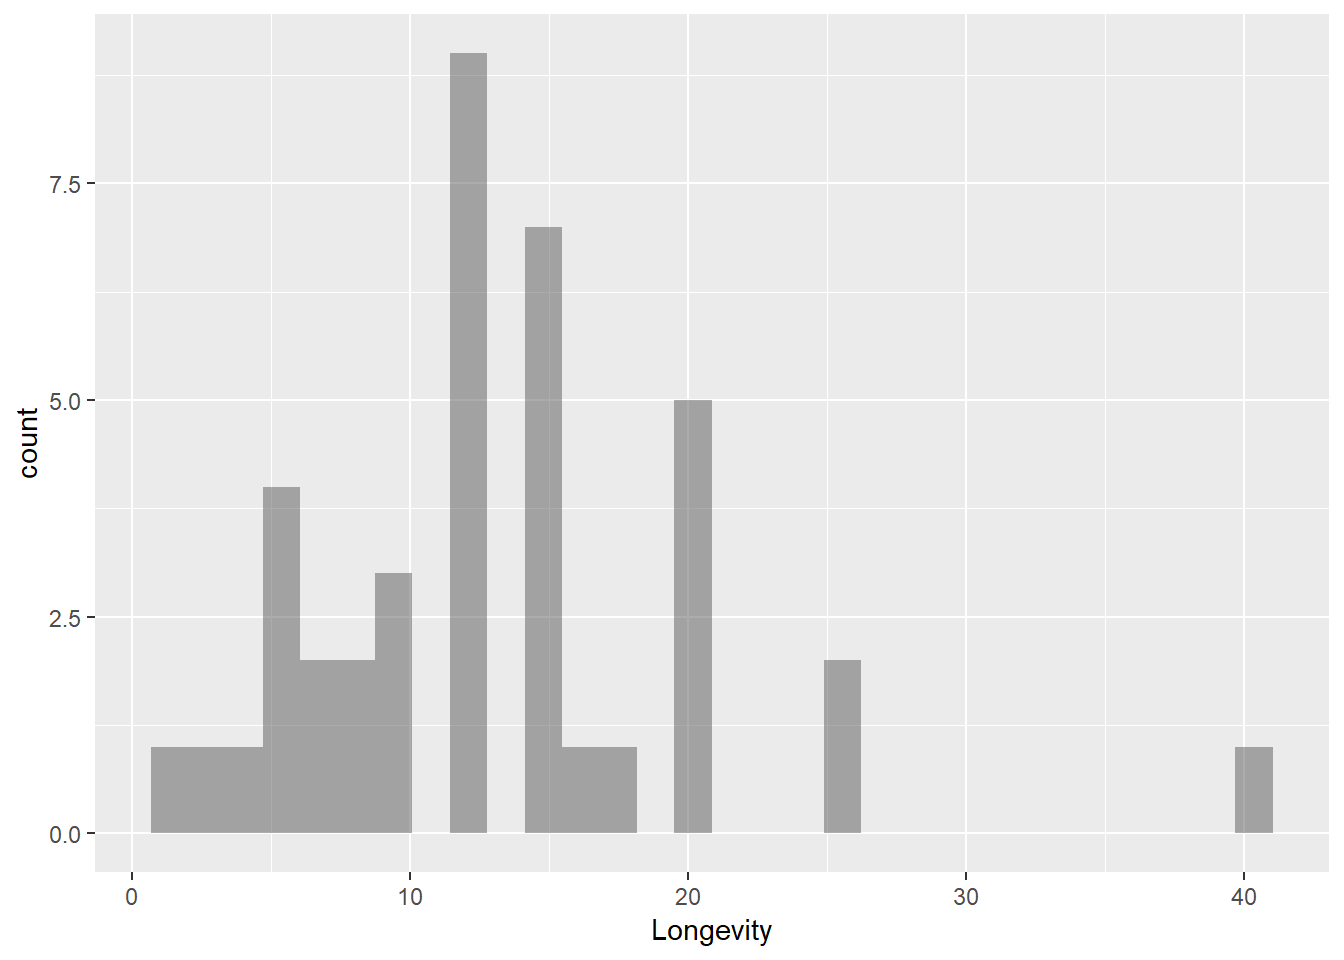
\includegraphics[width=0.65\linewidth]{Lock5WithR_files/figure-latex/Figure2.7b-3}

We can also describe the bins in terms of width instead of in terms of the number of bins. This is especially nice for count or other integer data.

\begin{Shaded}
\begin{Highlighting}[]
\KeywordTok{gf_histogram}\NormalTok{( }\OperatorTok{~}\StringTok{ }\NormalTok{Longevity, }\DataTypeTok{data =}\NormalTok{ MammalLongevity, }\DataTypeTok{binwidth =} \DecValTok{10}\NormalTok{)}
\end{Highlighting}
\end{Shaded}

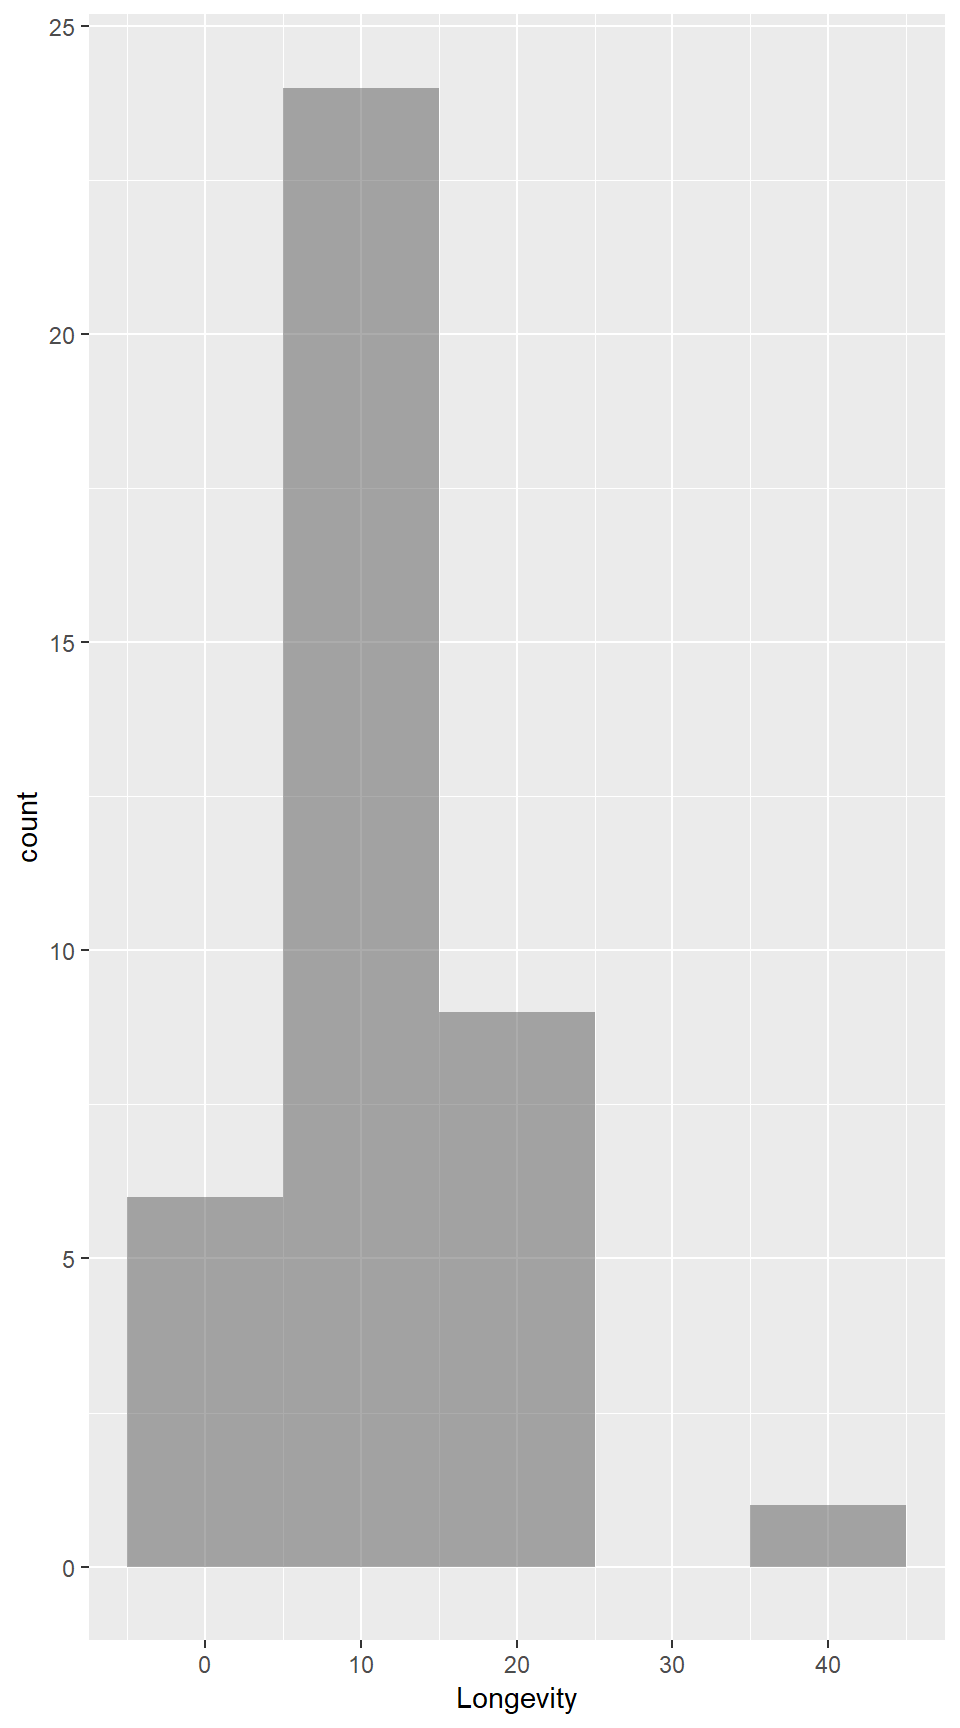
\includegraphics[width=0.65\linewidth]{Lock5WithR_files/figure-latex/Figure2.7c-1}

\begin{Shaded}
\begin{Highlighting}[]
\KeywordTok{gf_histogram}\NormalTok{( }\OperatorTok{~}\StringTok{ }\NormalTok{Longevity, }\DataTypeTok{data =}\NormalTok{ MammalLongevity, }\DataTypeTok{binwidth =} \DecValTok{5}\NormalTok{)}
\end{Highlighting}
\end{Shaded}

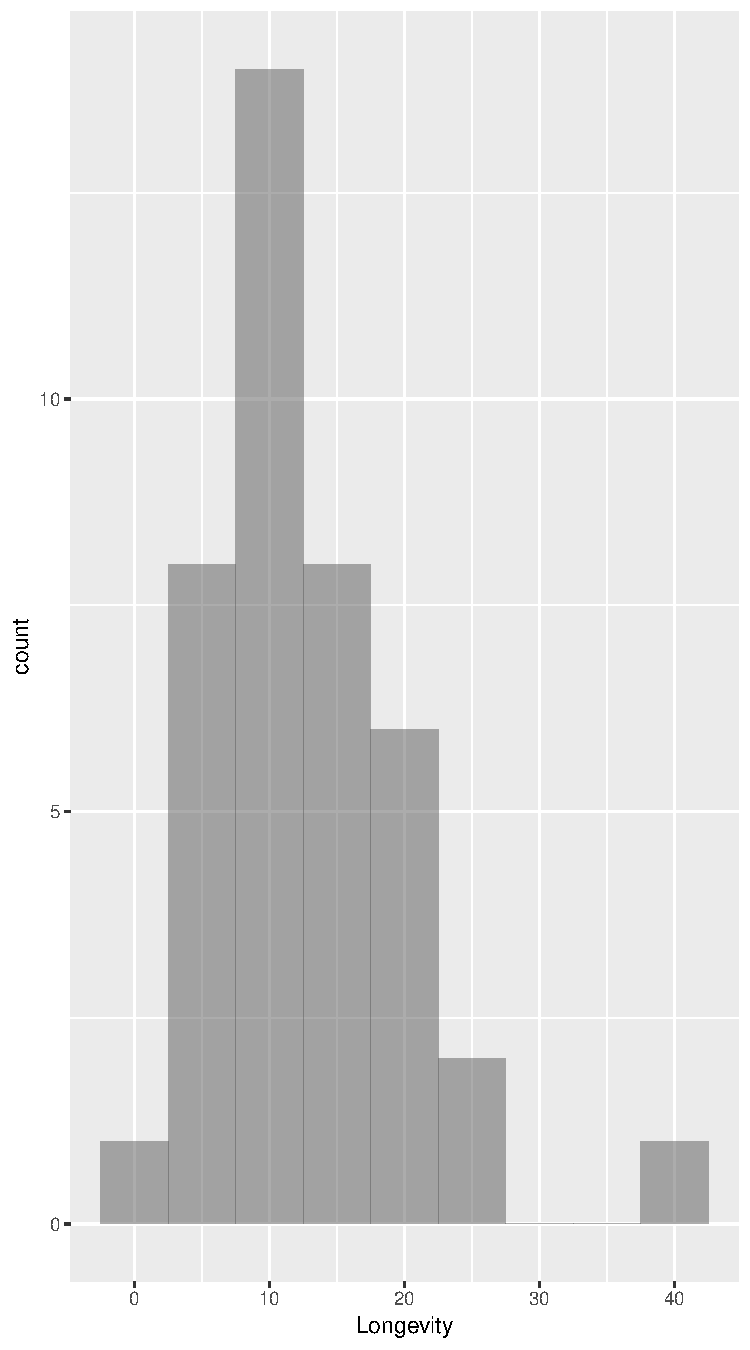
\includegraphics[width=0.65\linewidth]{Lock5WithR_files/figure-latex/Figure2.7c-2}

\begin{Shaded}
\begin{Highlighting}[]
\KeywordTok{gf_histogram}\NormalTok{( }\OperatorTok{~}\StringTok{ }\NormalTok{Longevity, }\DataTypeTok{data =}\NormalTok{ MammalLongevity, }\DataTypeTok{binwidth =} \DecValTok{2}\NormalTok{)}
\end{Highlighting}
\end{Shaded}

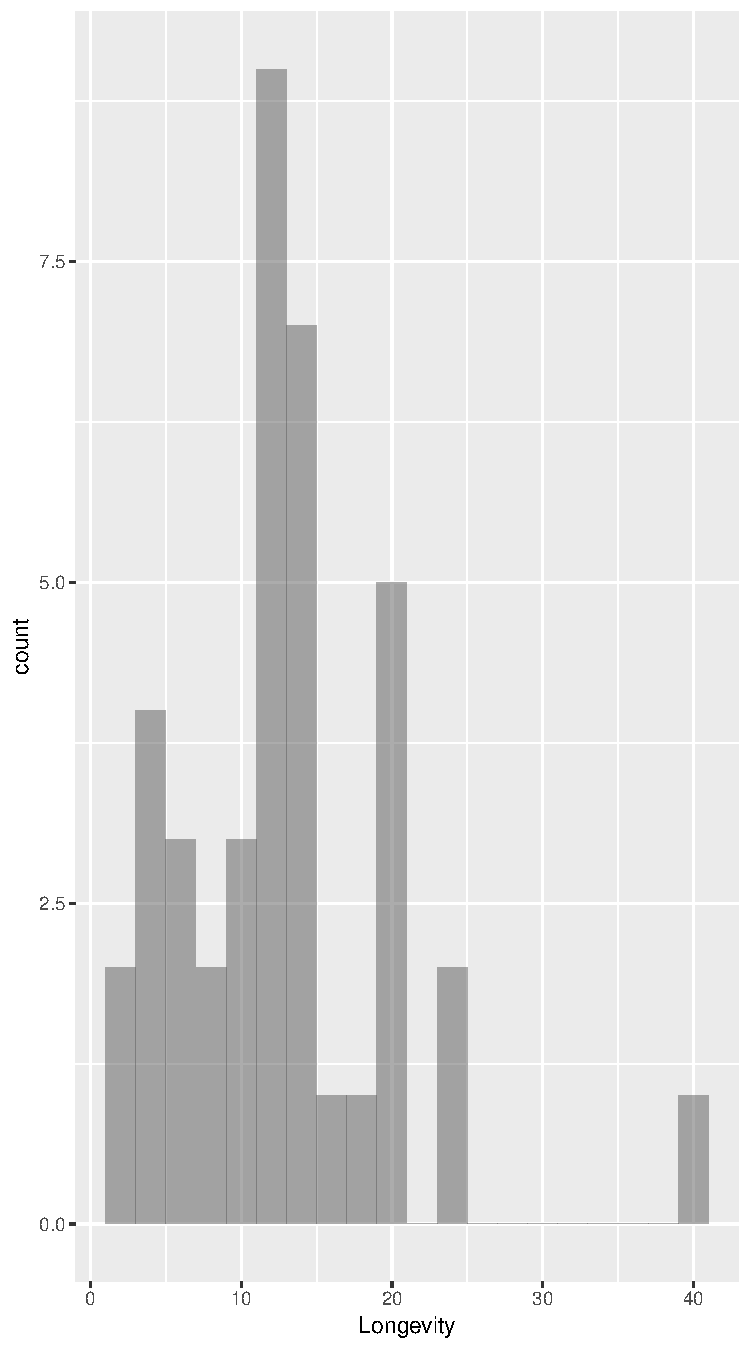
\includegraphics[width=0.65\linewidth]{Lock5WithR_files/figure-latex/Figure2.7c-3}

\hypertarget{figure-2.8}{%
\subsubsection{Figure 2.8}\label{figure-2.8}}

The various options available for the \texttt{gf\_histogram()()} function enable us to replicate Figure 2.8, some including closing, adding counts, labels, and limit to the y-axis (similar for x-axis). Using \texttt{gf\_dhistogram()()} measures the y-axis by density rather than count. This is useful for determing relative amounts.

\begin{Shaded}
\begin{Highlighting}[]
\KeywordTok{gf_histogram}\NormalTok{( }\OperatorTok{~}\StringTok{ }\NormalTok{Pulse, }\DataTypeTok{binwidth =} \DecValTok{5}\NormalTok{, }\DataTypeTok{data =}\NormalTok{ StudentSurvey)}
\end{Highlighting}
\end{Shaded}

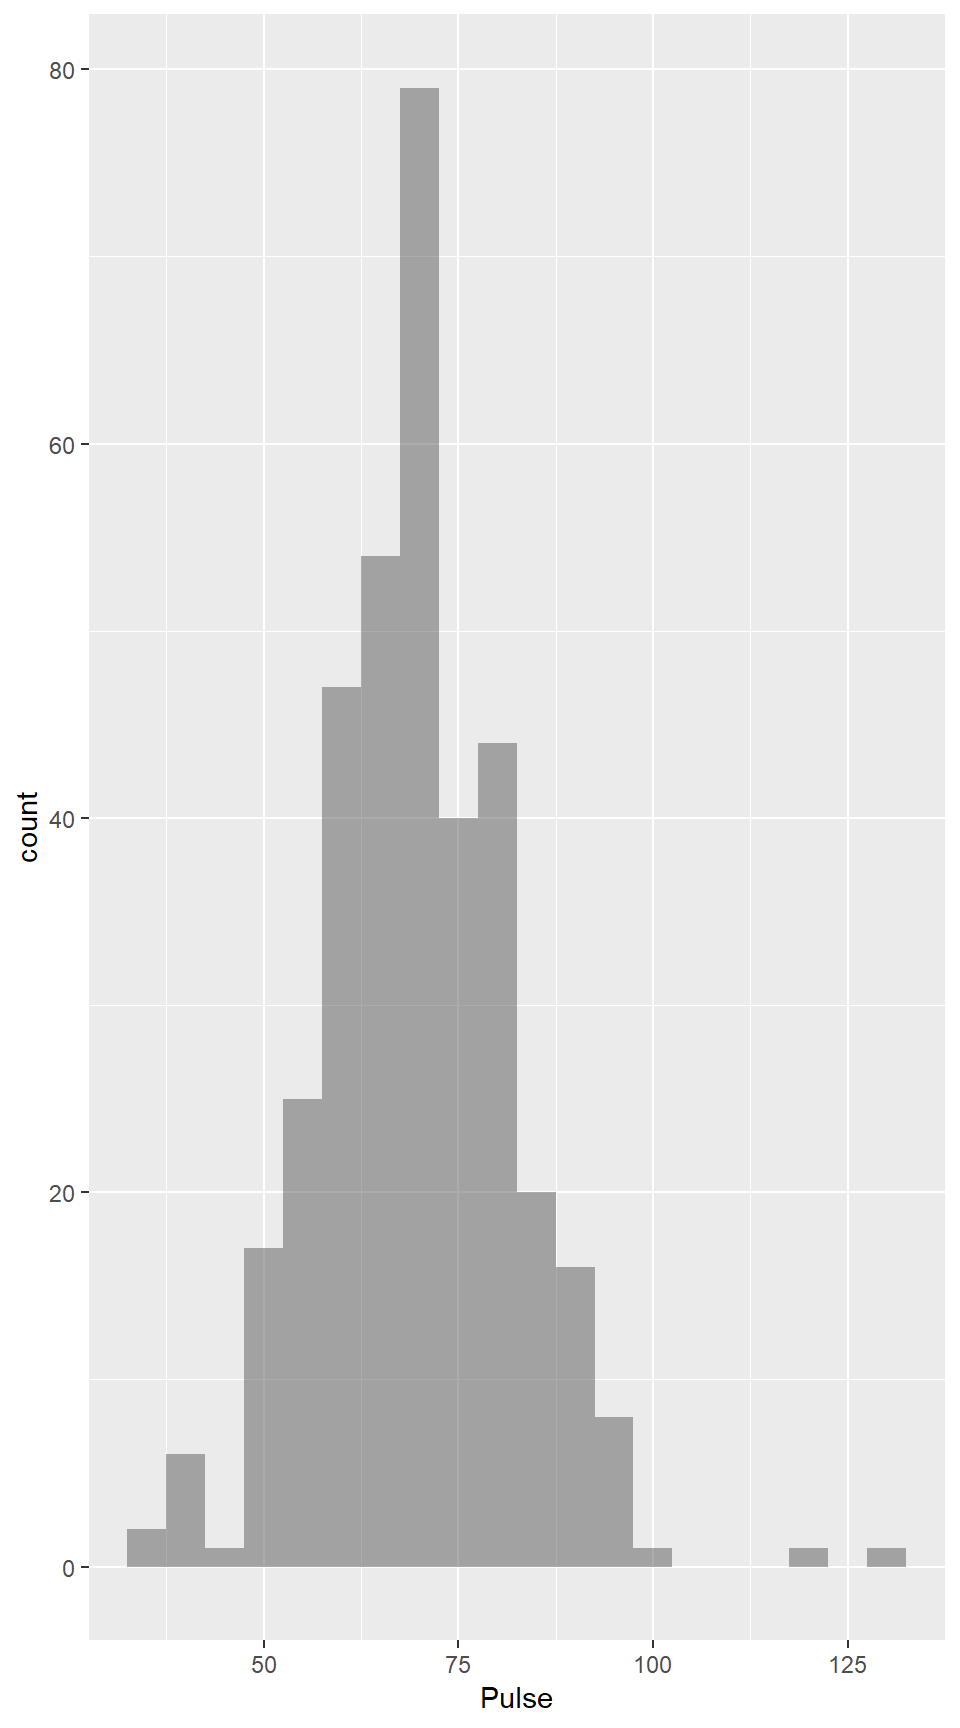
\includegraphics[width=0.65\linewidth]{Lock5WithR_files/figure-latex/Figure2.8-1}

\begin{Shaded}
\begin{Highlighting}[]
\KeywordTok{gf_histogram}\NormalTok{( }\OperatorTok{~}\StringTok{ }\NormalTok{Exercise, }\DataTypeTok{binwidth =} \DecValTok{2}\NormalTok{, }\DataTypeTok{closed =} \StringTok{'left'}\NormalTok{,}
              \DataTypeTok{data =}\NormalTok{ StudentSurvey)}
\end{Highlighting}
\end{Shaded}

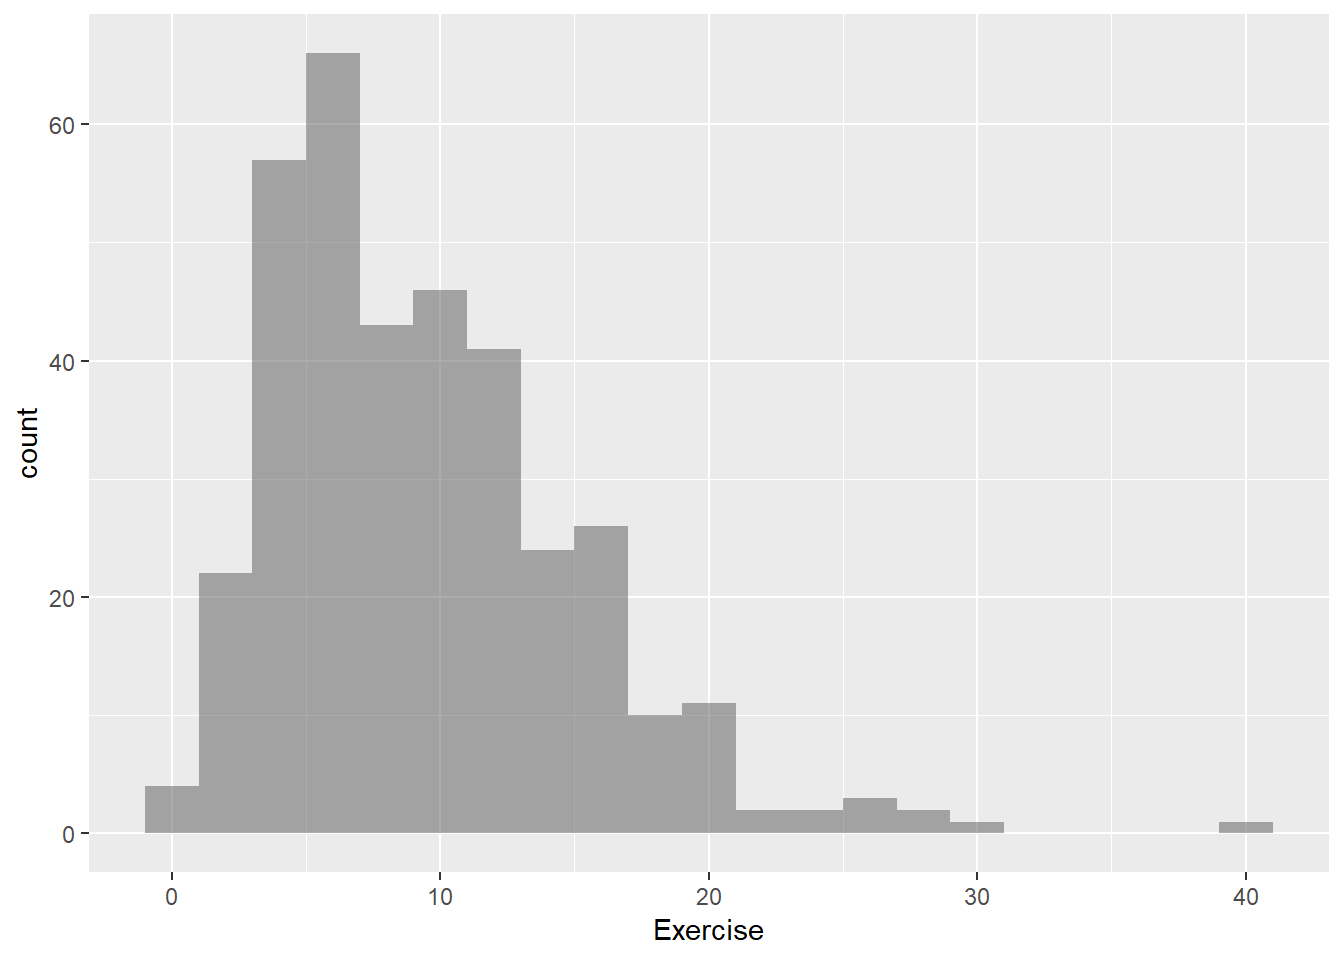
\includegraphics[width=0.65\linewidth]{Lock5WithR_files/figure-latex/Figure2.8-2}

\begin{Shaded}
\begin{Highlighting}[]
\KeywordTok{gf_dhistogram}\NormalTok{( }\OperatorTok{~}\NormalTok{Piercings, }\DataTypeTok{binwidth =} \DecValTok{1}\NormalTok{, }\DataTypeTok{data =}\NormalTok{ StudentSurvey)}
\end{Highlighting}
\end{Shaded}

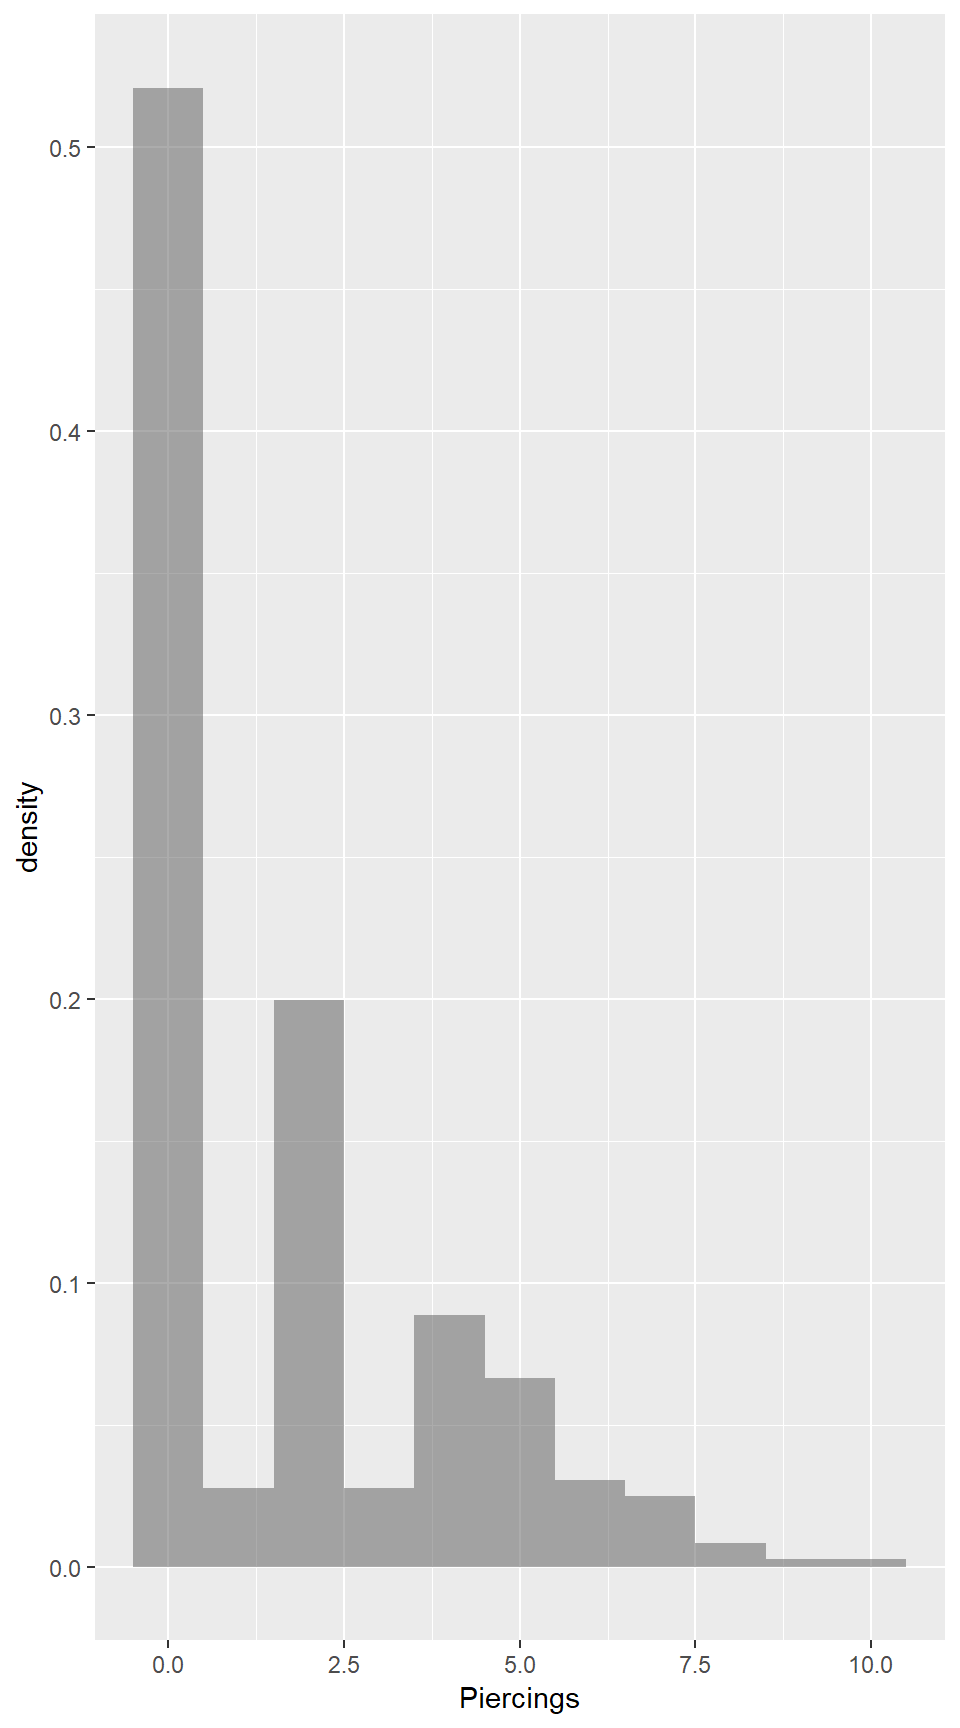
\includegraphics[width=0.65\linewidth]{Lock5WithR_files/figure-latex/Figure2.8-3}

Sometimes a \textbf{frequency polygon} provides a more useful view.
The only thing that changes is \texttt{gf\_histogram()()} becomes \texttt{gf\_freqpoly()()}.

\begin{Shaded}
\begin{Highlighting}[]
\KeywordTok{gf_freqpoly}\NormalTok{(..density.. }\OperatorTok{~}\StringTok{ }\NormalTok{Exercise, }\DataTypeTok{bins =} \DecValTok{10}\NormalTok{, }\DataTypeTok{data =}\NormalTok{ StudentSurvey)}
\end{Highlighting}
\end{Shaded}

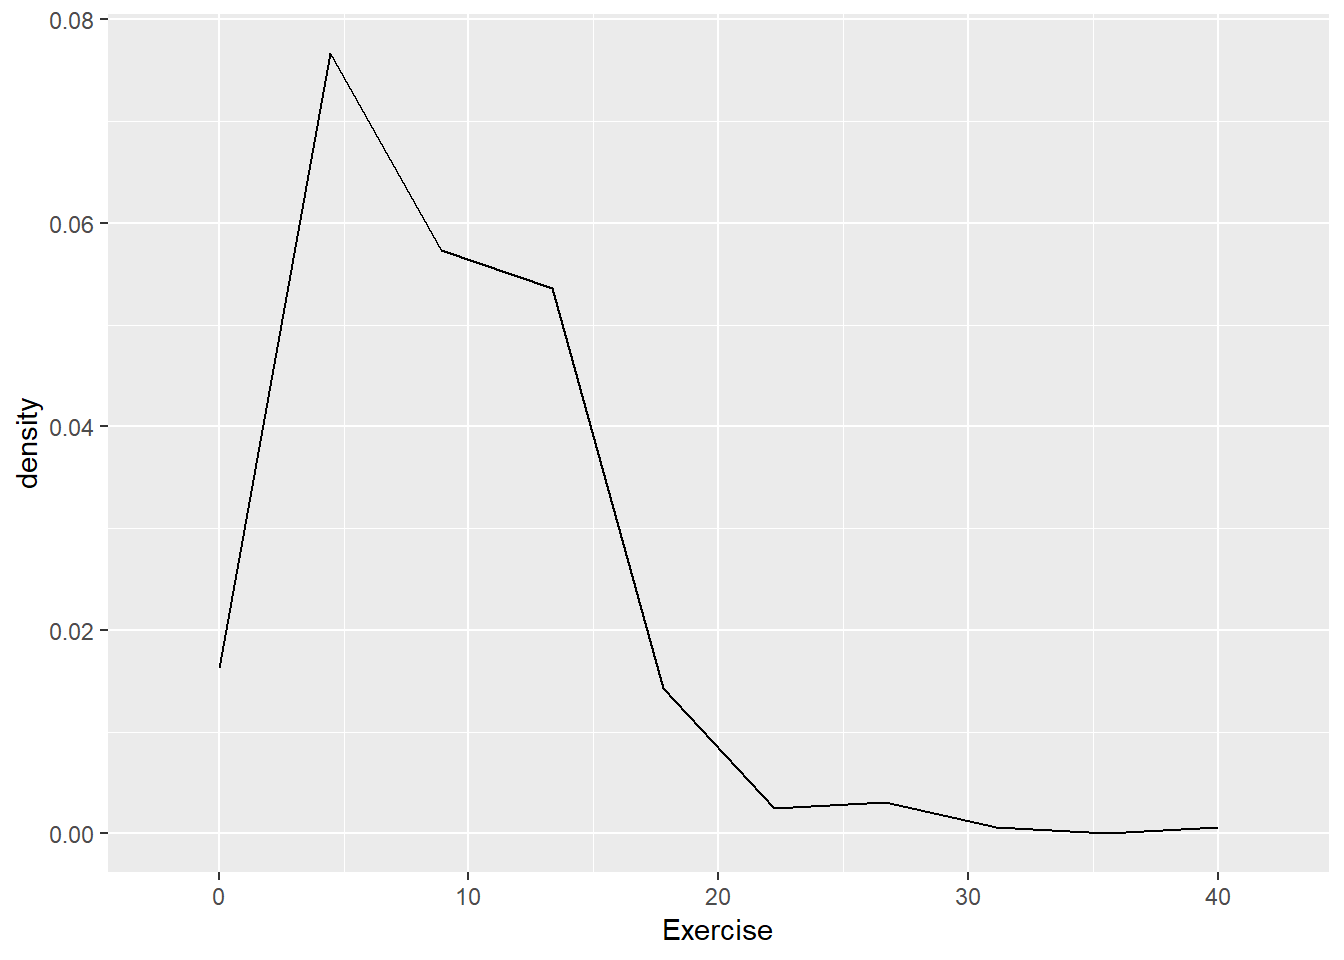
\includegraphics[width=0.65\linewidth]{Lock5WithR_files/figure-latex/freqpolygon-1}

What is a frequency polygon? The picture below shows how it is related to a histogram. The frequency polygon is just a dot-to-dot drawing through the centers of the tops of the bars of the histogram.

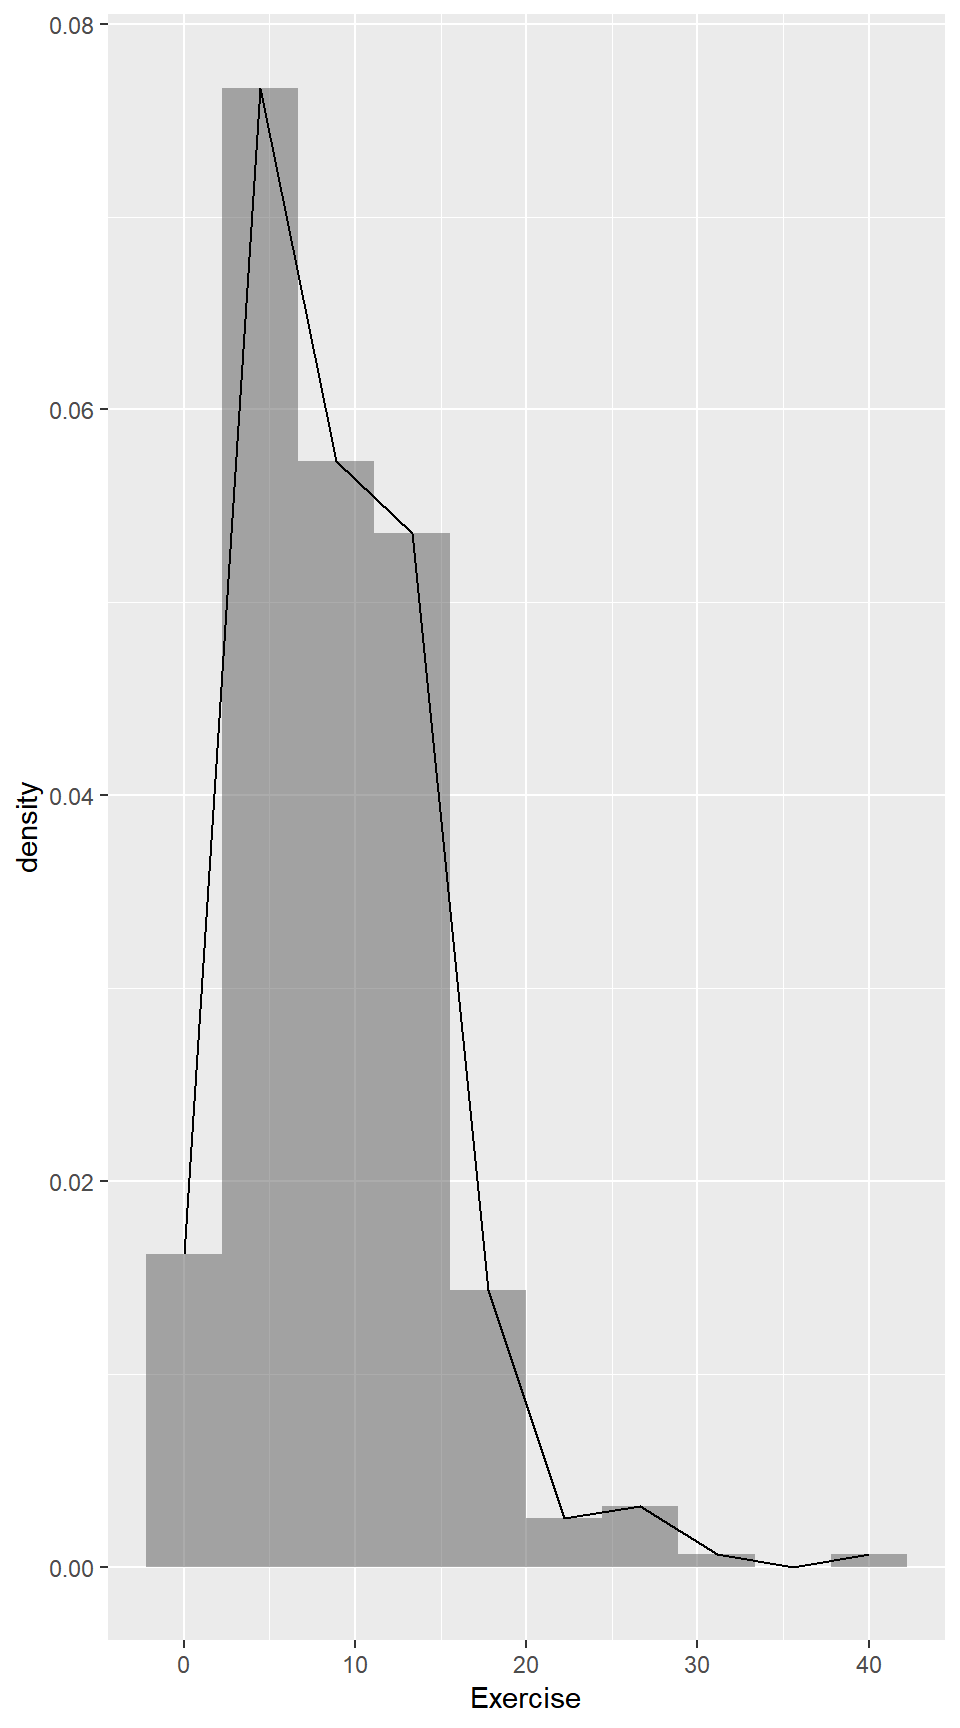
\includegraphics[width=0.65\linewidth]{Lock5WithR_files/figure-latex/freqpolygon-illustrated-1}

R also provides a ``smooth'' version called a density plot; just change the function name from \texttt{gf\_histogram()()} to \texttt{gf\_density()()}, also \texttt{gf\_dens()()} is a modified version of \texttt{gf\_density()} that isn't shaded in and may be useful for layering plots.

\begin{Shaded}
\begin{Highlighting}[]
\KeywordTok{gf_density}\NormalTok{( }\OperatorTok{~}\StringTok{ }\NormalTok{Longevity, }\DataTypeTok{data =}\NormalTok{ MammalLongevity)}
\end{Highlighting}
\end{Shaded}

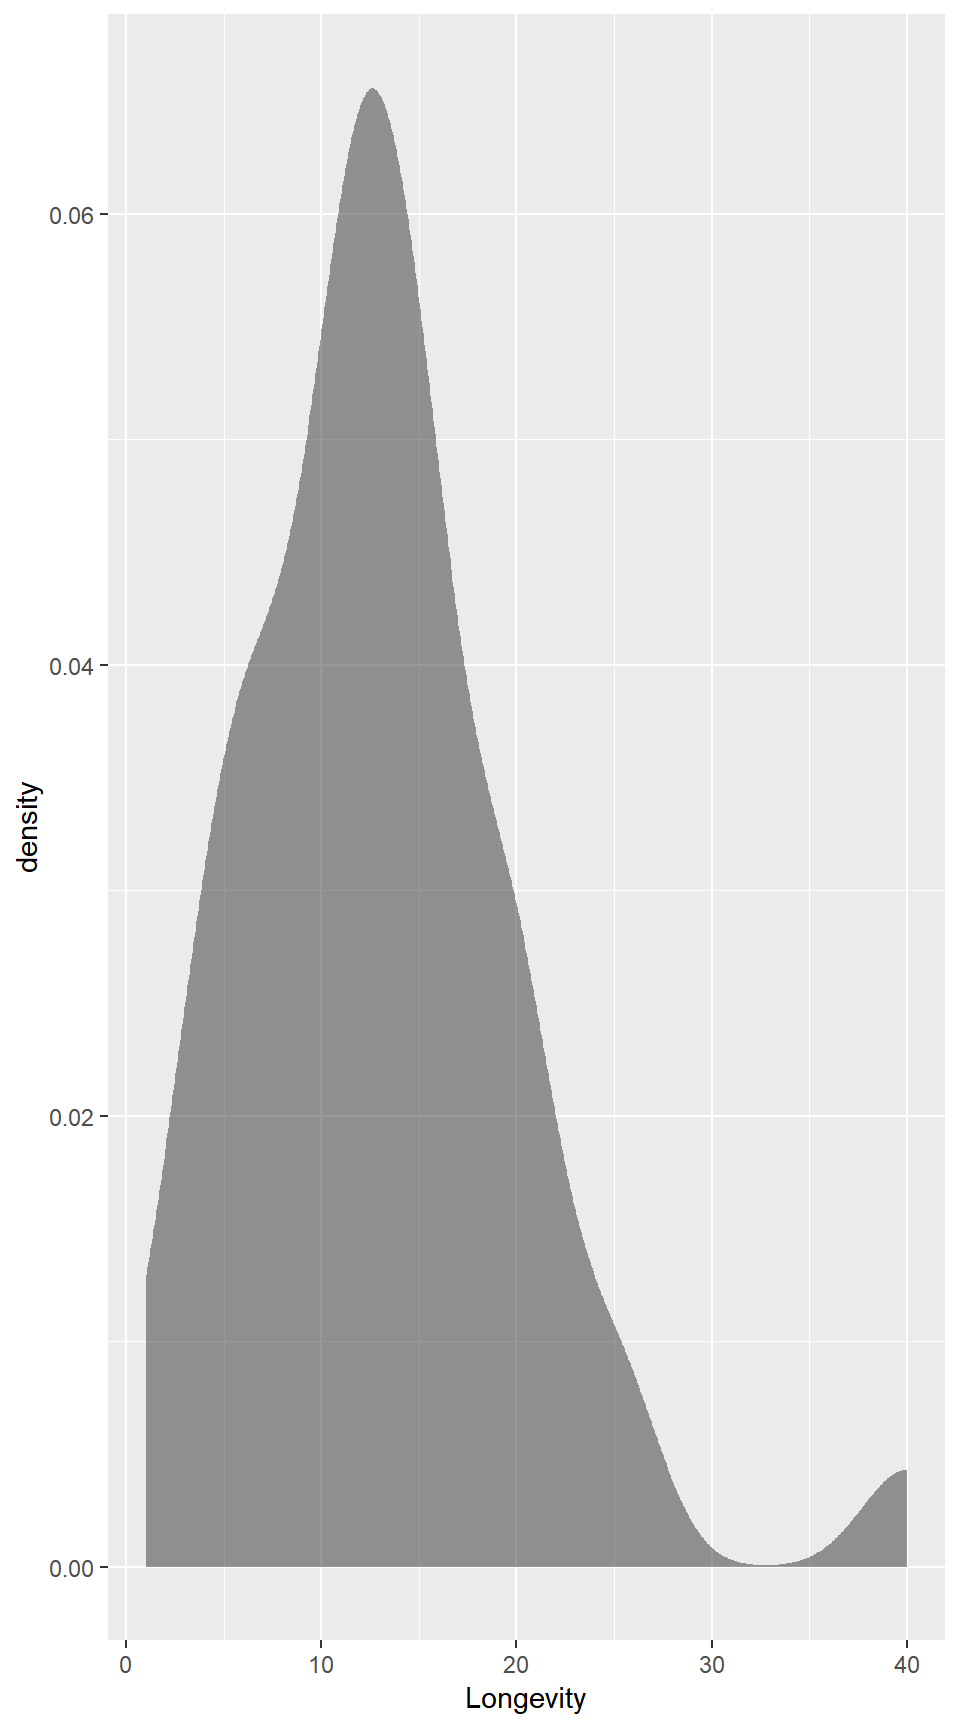
\includegraphics[width=0.65\linewidth]{Lock5WithR_files/figure-latex/densityplot-1}

\begin{Shaded}
\begin{Highlighting}[]
\KeywordTok{gf_dens}\NormalTok{( }\OperatorTok{~}\StringTok{ }\NormalTok{BirthRate, }\DataTypeTok{data =}\NormalTok{ AllCountries )}
\end{Highlighting}
\end{Shaded}

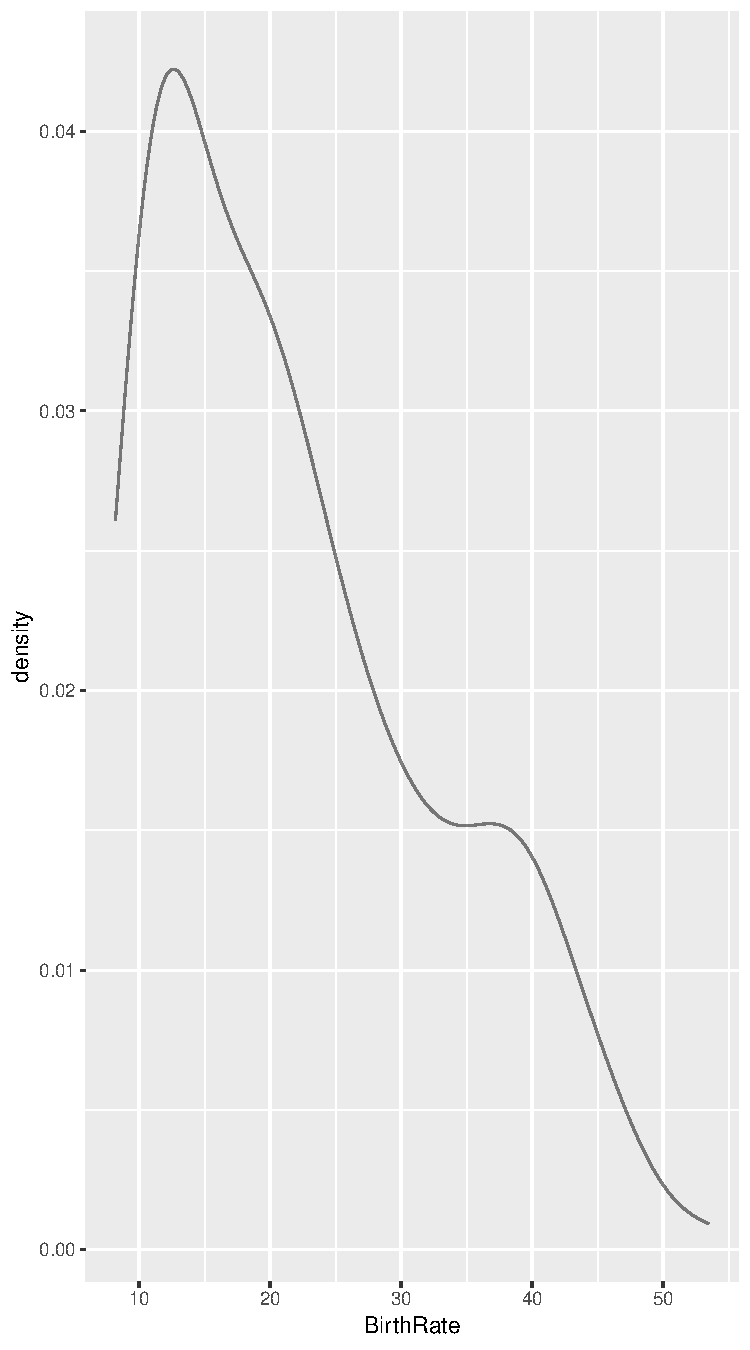
\includegraphics[width=0.65\linewidth]{Lock5WithR_files/figure-latex/densityplot-2}

If we make a histogram (or any of these other plots) of our data, we can describe the overall shape of the distribution. Keep in mind that the shape of a particular histogram may depend on the choice of bins. Choosing too many or too few bins can hide the true shape of the distribution. (When in doubt, make more than one histogram.)

Here are some words we use to describe shapes of distributions.

\begin{enumerate}
\tightlist
\item
  \textbf{symmetric} The left and right sides are mirror images of each other.
\item
  \textbf{skewed} The distribution stretches out farther in one direction than in the other.\\
  (We say the distribution is skewed toward the long tail.)
\item
  \textbf{uniform} The heights of all the bars are (roughly) the same.\\
  (So the data are equally likely to be anywhere within some range.)
\item
  \textbf{unimodal} There is one major ``bump'' where there is a lot of data.
\item
  \textbf{bimodal} There are two ``bumps''.
\item
  \textbf{outlier} An observation that does not fit the overall pattern of the rest of
  the data.
\end{enumerate}

\hypertarget{the-center-of-a-distribution}{%
\subsection{The Center of a Distribution}\label{the-center-of-a-distribution}}

Recall that a statistic is a number computed from data. The \textbf{mean} and the \textbf{median} are key statistics which describe the center of a distribution. We can see through Example 2.11 that numerical summaries are computed using the same template as graphical summaries.

Note that the example asks about subsets of {ICUAdmissions}--specifically about 20-year-old and 55-year-old patients. In this case, we can manipulate the data (to name a new data set) with the subset command. Here are some examples.

\begin{enumerate}
\item
\begin{verbatim}
Select only the males from the <span style="color:blue">ICUAdmissions</span> data set.
\end{verbatim}
\end{enumerate}

\begin{Shaded}
\begin{Highlighting}[]
\KeywordTok{head}\NormalTok{(ICUAdmissions, }\DecValTok{2}\NormalTok{)}
\end{Highlighting}
\end{Shaded}

\begin{verbatim}
##   ID Status Age Sex Race Service Cancer Renal Infection CPR Systolic
## 1  8      0  27   1    1       0      0     0         1   0      142
## 2 12      0  59   0    1       0      0     0         0   0      112
##   HeartRate Previous Type Fracture PO2 PH PCO2 Bicarbonate Creatinine
## 1        88        0    1        0   0  0    0           0          0
## 2        80        1    1        0   0  0    0           0          0
##   Consciousness status    sex  race service cancer renal infection cpr
## 1             1  Lived Female White Medical     No    No       Yes  No
## 2             1  Lived   Male White Medical     No    No        No  No
##   previous      type pO2low pO2 pHlow pH pCO2hi pCO2 bicarbonateLow
## 1       No Emergency     No  Hi    No Hi     No  Low             No
## 2      Yes Emergency     No  Hi    No Hi     No  Low             No
##   bicarbonate creatinineHi creatinine consciousness
## 1          Hi           No        Low     Conscious
## 2          Hi           No        Low     Conscious
\end{verbatim}

\begin{Shaded}
\begin{Highlighting}[]
\KeywordTok{tally}\NormalTok{( }\OperatorTok{~}\StringTok{ }\NormalTok{sex, }\DataTypeTok{data =}\NormalTok{ ICUAdmissions) }
\end{Highlighting}
\end{Shaded}

\begin{verbatim}
## sex
## Female   Male 
##     76    124
\end{verbatim}

\begin{Shaded}
\begin{Highlighting}[]
\NormalTok{ICUMales <-}\StringTok{ }\KeywordTok{subset}\NormalTok{(ICUAdmissions, sex }\OperatorTok{==}\StringTok{ "Male"}\NormalTok{) }\CommentTok{# notice the double =}
\KeywordTok{tally}\NormalTok{( }\OperatorTok{~}\StringTok{ }\NormalTok{sex, }\DataTypeTok{data =}\NormalTok{ ICUMales)}
\end{Highlighting}
\end{Shaded}

\begin{verbatim}
## sex
## Female   Male 
##      0    124
\end{verbatim}

\begin{verbatim}
#.      Select only the subjects over 50:
\end{verbatim}

\begin{Shaded}
\begin{Highlighting}[]
\NormalTok{ICUOld <-}\StringTok{ }\KeywordTok{subset}\NormalTok{(ICUAdmissions, Age }\OperatorTok{>}\StringTok{ }\DecValTok{50}\NormalTok{) }
\end{Highlighting}
\end{Shaded}

The \texttt{subset()()} function can use any condition that evaluates to TRUE or FALSE for each row (case) in the data set.

\hypertarget{example-2.11}{%
\subsubsection{Example 2.11}\label{example-2.11}}

\begin{Shaded}
\begin{Highlighting}[]
\NormalTok{ICU20 <-}\StringTok{ }\KeywordTok{subset}\NormalTok{(ICUAdmissions, Age }\OperatorTok{==}\StringTok{ "20"}\NormalTok{)}
\KeywordTok{mean}\NormalTok{( }\OperatorTok{~}\StringTok{ }\NormalTok{HeartRate, }\DataTypeTok{data =}\NormalTok{ ICU20)}
\end{Highlighting}
\end{Shaded}

\begin{verbatim}
## [1] 82.2
\end{verbatim}

\begin{Shaded}
\begin{Highlighting}[]
\KeywordTok{median}\NormalTok{( }\OperatorTok{~}\StringTok{ }\NormalTok{HeartRate, }\DataTypeTok{data =}\NormalTok{ ICU20)}
\end{Highlighting}
\end{Shaded}

\begin{verbatim}
## [1] 80
\end{verbatim}

\begin{Shaded}
\begin{Highlighting}[]
\NormalTok{ICU55 =}\StringTok{ }\KeywordTok{subset}\NormalTok{(ICUAdmissions, Age }\OperatorTok{==}\StringTok{ "55"}\NormalTok{)}
\KeywordTok{mean}\NormalTok{( }\OperatorTok{~}\StringTok{ }\NormalTok{HeartRate, }\DataTypeTok{data =}\NormalTok{ ICU55)}
\end{Highlighting}
\end{Shaded}

\begin{verbatim}
## [1] 108.5
\end{verbatim}

\begin{Shaded}
\begin{Highlighting}[]
\KeywordTok{median}\NormalTok{( }\OperatorTok{~}\StringTok{ }\NormalTok{HeartRate, }\DataTypeTok{data =}\NormalTok{ ICU55)}
\end{Highlighting}
\end{Shaded}

\begin{verbatim}
## [1] 106
\end{verbatim}

\hypertarget{resistance}{%
\subsection{Resistance}\label{resistance}}

\hypertarget{figure-2.10}{%
\subsubsection{Figure 2.10}\label{figure-2.10}}

\begin{Shaded}
\begin{Highlighting}[]
\KeywordTok{head}\NormalTok{(FloridaLakes)}
\end{Highlighting}
\end{Shaded}

\begin{verbatim}
##   ID         Lake Alkalinity  pH Calcium Chlorophyll AvgMercury NumSamples
## 1  1    Alligator        5.9 6.1     3.0         0.7       1.23          5
## 2  2        Annie        3.5 5.1     1.9         3.2       1.33          7
## 3  3       Apopka      116.0 9.1    44.1       128.3       0.04          6
## 4  4 Blue Cypress       39.4 6.9    16.4         3.5       0.44         12
## 5  5        Brick        2.5 4.6     2.9         1.8       1.20         12
## 6  6       Bryant       19.6 7.3     4.5        44.1       0.27         14
##   MinMercury MaxMercury ThreeYrStdMercury AgeData
## 1       0.85       1.43              1.53       1
## 2       0.92       1.90              1.33       0
## 3       0.04       0.06              0.04       0
## 4       0.13       0.84              0.44       0
## 5       0.69       1.50              1.33       1
## 6       0.04       0.48              0.25       1
\end{verbatim}

\begin{Shaded}
\begin{Highlighting}[]
\KeywordTok{gf_histogram}\NormalTok{( }\OperatorTok{~}\StringTok{ }\NormalTok{Alkalinity, }\DataTypeTok{binwidth =} \DecValTok{10}\NormalTok{, }\DataTypeTok{data =}\NormalTok{ FloridaLakes)}
\end{Highlighting}
\end{Shaded}

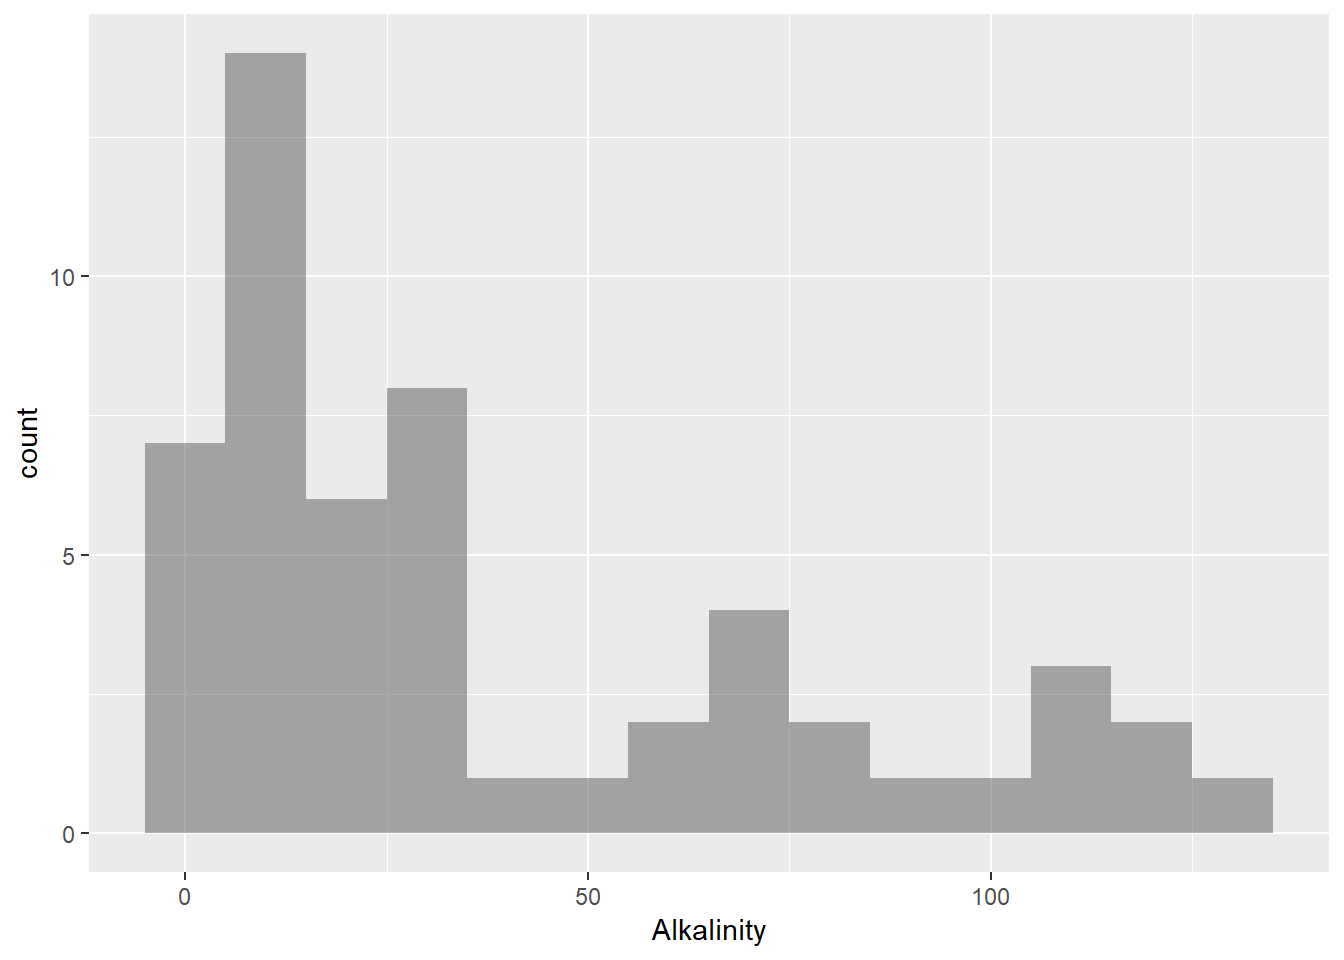
\includegraphics[width=0.65\linewidth]{Lock5WithR_files/figure-latex/Figure2.10-1}

\hypertarget{example-2.14}{%
\subsubsection{Example 2.14}\label{example-2.14}}

\begin{Shaded}
\begin{Highlighting}[]
\KeywordTok{mean}\NormalTok{( }\OperatorTok{~}\StringTok{ }\NormalTok{Alkalinity, }\DataTypeTok{data =}\NormalTok{ FloridaLakes)}
\end{Highlighting}
\end{Shaded}

\begin{verbatim}
## [1] 37.53019
\end{verbatim}

\begin{Shaded}
\begin{Highlighting}[]
\KeywordTok{median}\NormalTok{( }\OperatorTok{~}\StringTok{ }\NormalTok{Alkalinity, }\DataTypeTok{data =}\NormalTok{ FloridaLakes)}
\end{Highlighting}
\end{Shaded}

\begin{verbatim}
## [1] 19.6
\end{verbatim}

\hypertarget{one-quantitative-variable-measures-of-spread}{%
\section{One Quantitative Variable: Measures of Spread}\label{one-quantitative-variable-measures-of-spread}}

In the previous section, we investigated center summary statistics. In this section, we will cover some other important statistics.

\hypertarget{example-2.15}{%
\subsubsection{Example 2.15}\label{example-2.15}}

\begin{Shaded}
\begin{Highlighting}[]
\KeywordTok{summary}\NormalTok{(April14Temps)}
\end{Highlighting}
\end{Shaded}

\begin{verbatim}
##       Year        DesMoines      SanFrancisco  
##  Min.   :1995   Min.   :37.20   Min.   :48.70  
##  1st Qu.:1999   1st Qu.:44.40   1st Qu.:51.30  
##  Median :2002   Median :54.50   Median :54.00  
##  Mean   :2002   Mean   :54.49   Mean   :54.01  
##  3rd Qu.:2006   3rd Qu.:61.27   3rd Qu.:55.90  
##  Max.   :2010   Max.   :74.90   Max.   :61.00
\end{verbatim}

\begin{Shaded}
\begin{Highlighting}[]
\KeywordTok{favstats}\NormalTok{( }\OperatorTok{~}\StringTok{ }\NormalTok{DesMoines, }\DataTypeTok{data =}\NormalTok{ April14Temps) }\CommentTok{# some favorite statistics}
\end{Highlighting}
\end{Shaded}

\begin{verbatim}
##   min   Q1 median     Q3  max    mean      sd  n missing
##  37.2 44.4   54.5 61.275 74.9 54.4875 11.7303 16       0
\end{verbatim}

\begin{Shaded}
\begin{Highlighting}[]
\KeywordTok{favstats}\NormalTok{( }\OperatorTok{~}\StringTok{ }\NormalTok{SanFrancisco, }\DataTypeTok{data =}\NormalTok{ April14Temps)}
\end{Highlighting}
\end{Shaded}

\begin{verbatim}
##   min   Q1 median   Q3 max    mean       sd  n missing
##  48.7 51.3     54 55.9  61 54.0125 3.376956 16       0
\end{verbatim}

\hypertarget{standard-deviation}{%
\subsection{Standard Deviation}\label{standard-deviation}}

The density plots of the temperatures of Des Moines and San Francisco reveal that Des Moines has a greater \emph{variability} or \emph{spread}.

\hypertarget{figure-2.18}{%
\subsubsection{Figure 2.18}\label{figure-2.18}}

The \argument{dotsize} argument controls \texttt{character\ expansion"\ and\ can\ be\ used\ to\ make\ the\ plotting}characters" larger or smaller by specifying the scaling ratio. \argument{stackratio} allows you to adjust the vertical distance between points. Chaining \function{gf_lims()} lets you set the limits for the x and y-axes.

\begin{Shaded}
\begin{Highlighting}[]
\KeywordTok{gf_dotplot}\NormalTok{( }\OperatorTok{~}\StringTok{ }\NormalTok{DesMoines, }\DataTypeTok{binwidth =} \DecValTok{1}\NormalTok{, }\DataTypeTok{dotsize =} \DecValTok{2}\NormalTok{, }\DataTypeTok{stackratio =} \DecValTok{3}\NormalTok{,}
            \DataTypeTok{data =}\NormalTok{ April14Temps) }\OperatorTok\StringTok{ }\KeywordTok{gf_lims}\NormalTok{(}\DataTypeTok{x =} \KeywordTok{c}\NormalTok{(}\DecValTok{35}\NormalTok{, }\DecValTok{80}\NormalTok{))}
\end{Highlighting}
\end{Shaded}

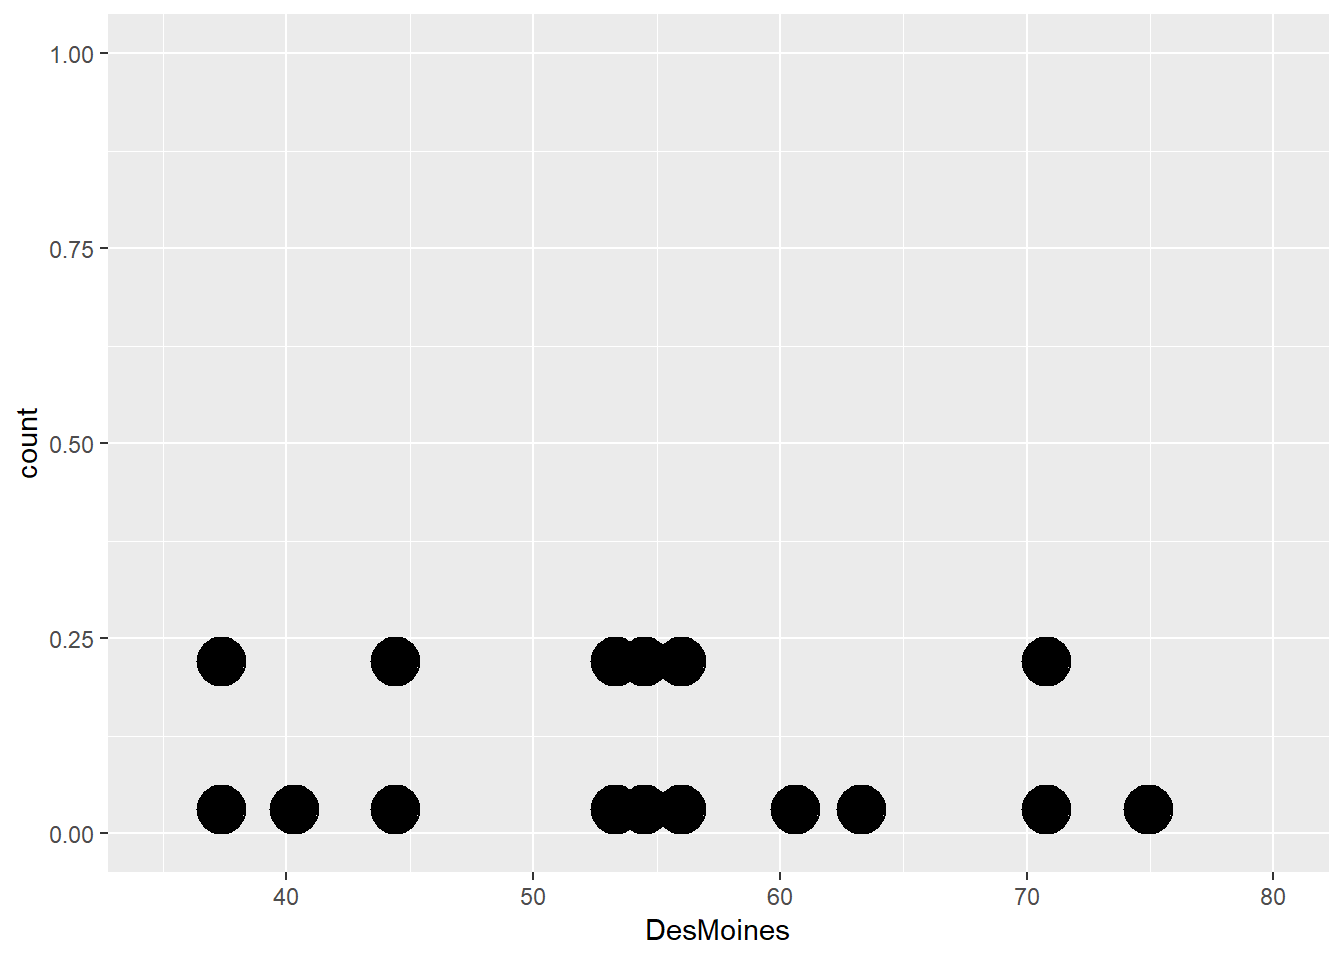
\includegraphics[width=0.65\linewidth]{Lock5WithR_files/figure-latex/Figure2.18-1}

\begin{Shaded}
\begin{Highlighting}[]
\KeywordTok{gf_dotplot}\NormalTok{( }\OperatorTok{~}\StringTok{ }\NormalTok{SanFrancisco, }\DataTypeTok{binwidth =} \DecValTok{1}\NormalTok{, }\DataTypeTok{dotsize =} \FloatTok{.5}\NormalTok{, }\DataTypeTok{stackratio =} \DecValTok{2}\NormalTok{, }
            \DataTypeTok{data =}\NormalTok{ April14Temps) }\OperatorTok\StringTok{ }\KeywordTok{gf_lims}\NormalTok{(}\DataTypeTok{x =} \KeywordTok{c}\NormalTok{(}\DecValTok{45}\NormalTok{, }\DecValTok{65}\NormalTok{))}
\end{Highlighting}
\end{Shaded}

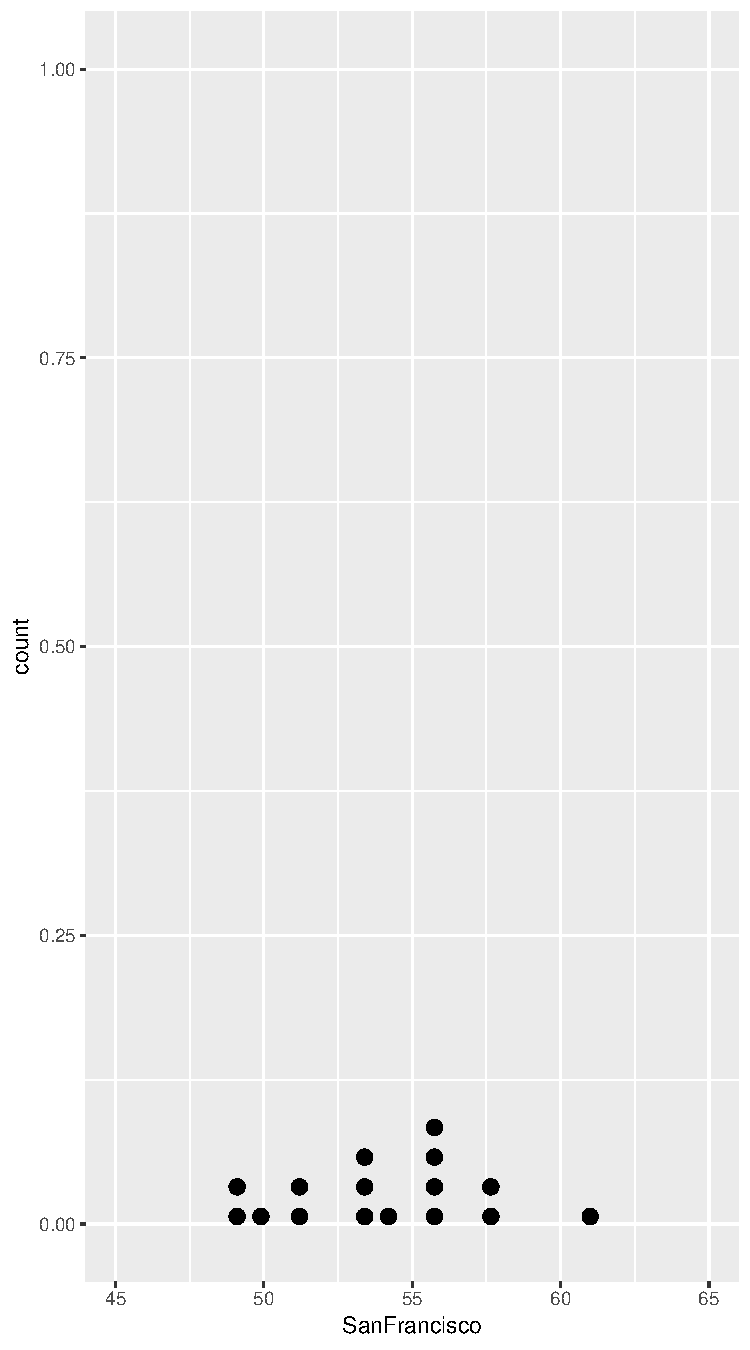
\includegraphics[width=0.65\linewidth]{Lock5WithR_files/figure-latex/Figure2.18-2}

\hypertarget{example-2.16}{%
\subsubsection{Example 2.16}\label{example-2.16}}

Although both \texttt{summary()()} and \texttt{favstats()()} calculate the \textbf{standard deviation} of a variable, we can also use \texttt{sd()()} to find just the standard deviation.

\begin{Shaded}
\begin{Highlighting}[]
\KeywordTok{sd}\NormalTok{( }\OperatorTok{~}\StringTok{ }\NormalTok{DesMoines, }\DataTypeTok{data =}\NormalTok{ April14Temps)        }
\end{Highlighting}
\end{Shaded}

\begin{verbatim}
## [1] 11.7303
\end{verbatim}

\begin{Shaded}
\begin{Highlighting}[]
\KeywordTok{sd}\NormalTok{( }\OperatorTok{~}\StringTok{ }\NormalTok{SanFrancisco, }\DataTypeTok{data =}\NormalTok{ April14Temps)}
\end{Highlighting}
\end{Shaded}

\begin{verbatim}
## [1] 3.376956
\end{verbatim}

\begin{Shaded}
\begin{Highlighting}[]
\KeywordTok{var}\NormalTok{( }\OperatorTok{~}\StringTok{ }\NormalTok{DesMoines, }\DataTypeTok{data =}\NormalTok{ April14Temps)        }\CommentTok{# variance = sd^2}
\end{Highlighting}
\end{Shaded}

\begin{verbatim}
## [1] 137.5998
\end{verbatim}

\hypertarget{example-2.17}{%
\subsubsection{Example 2.17}\label{example-2.17}}

To see that the distribution is indeed symmetric and approximately bell-shaped, you can chain the function \texttt{gf\_dens()()}. It can be helpful to set alpha (the transparency argument) lower than 1 to make the plot easier to read.

\begin{Shaded}
\begin{Highlighting}[]
\KeywordTok{gf_dhistogram}\NormalTok{( }\OperatorTok{~}\StringTok{ }\NormalTok{Pulse, }\DataTypeTok{data =}\NormalTok{ StudentSurvey, }\DataTypeTok{alpha =} \FloatTok{.5}\NormalTok{) }\OperatorTok\StringTok{ }\KeywordTok{gf_dens}\NormalTok{( }\OperatorTok{~}\StringTok{ }\NormalTok{Pulse)}
\end{Highlighting}
\end{Shaded}

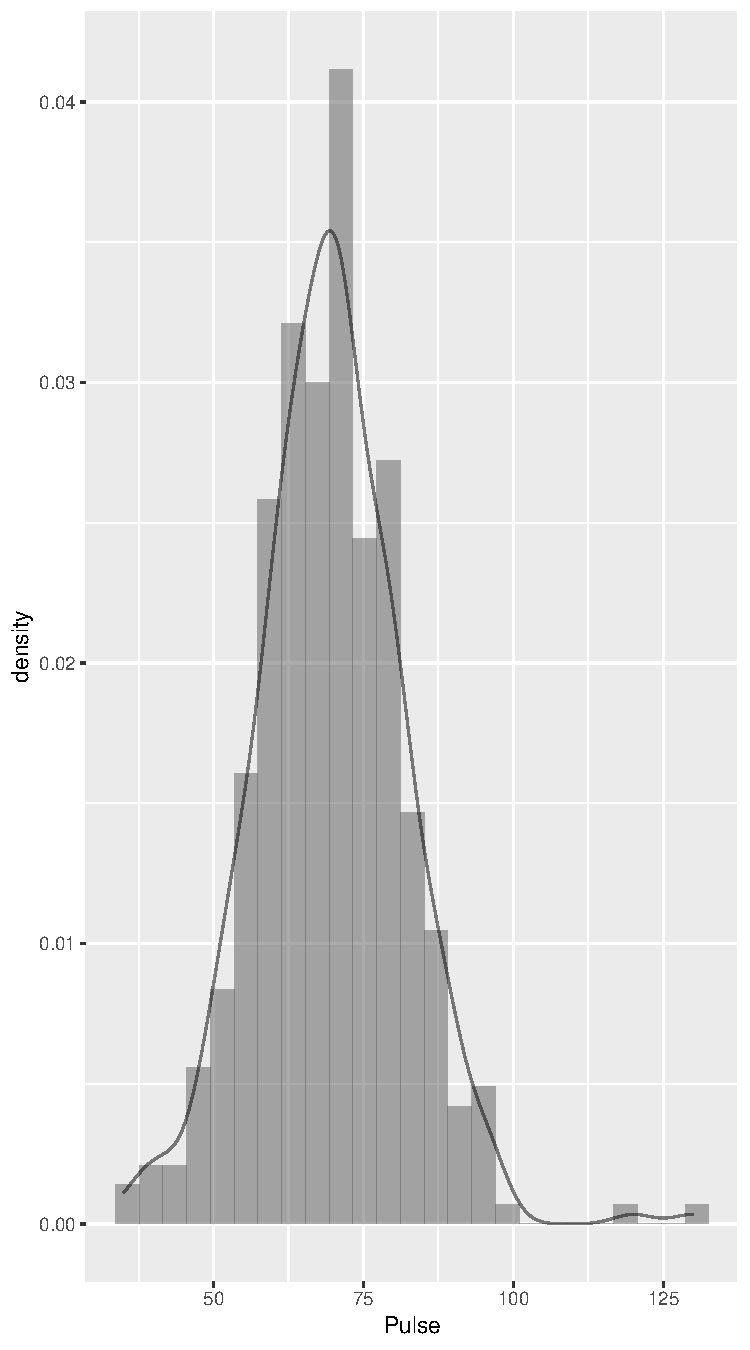
\includegraphics[width=0.65\linewidth]{Lock5WithR_files/figure-latex/Example2.17-1}

\begin{Shaded}
\begin{Highlighting}[]
\NormalTok{mean <-}\StringTok{ }\KeywordTok{mean}\NormalTok{( }\OperatorTok{~}\StringTok{ }\NormalTok{Pulse, }\DataTypeTok{data =}\NormalTok{ StudentSurvey); mean}
\end{Highlighting}
\end{Shaded}

\begin{verbatim}
## [1] 69.57459
\end{verbatim}

\begin{Shaded}
\begin{Highlighting}[]
\NormalTok{sd <-}\StringTok{ }\KeywordTok{sd}\NormalTok{( }\OperatorTok{~}\StringTok{ }\NormalTok{Pulse, }\DataTypeTok{data =}\NormalTok{ StudentSurvey); sd}
\end{Highlighting}
\end{Shaded}

\begin{verbatim}
## [1] 12.20514
\end{verbatim}

\begin{Shaded}
\begin{Highlighting}[]
\NormalTok{mean }\OperatorTok{-}\StringTok{ }\DecValTok{2}\OperatorTok{*}\NormalTok{sd}
\end{Highlighting}
\end{Shaded}

\begin{verbatim}
## [1] 45.16431
\end{verbatim}

\begin{Shaded}
\begin{Highlighting}[]
\NormalTok{mean }\OperatorTok{+}\StringTok{ }\DecValTok{2}\OperatorTok{*}\NormalTok{sd}
\end{Highlighting}
\end{Shaded}

\begin{verbatim}
## [1] 93.98486
\end{verbatim}

\hypertarget{figure-2.20}{%
\subsubsection{Figure 2.20}\label{figure-2.20}}

\begin{Shaded}
\begin{Highlighting}[]
\KeywordTok{gf_dhistogram}\NormalTok{( }\OperatorTok{~}\StringTok{ }\NormalTok{Sales, }\DataTypeTok{binwidth =} \DecValTok{25}\NormalTok{, }\DataTypeTok{data =}\NormalTok{ RetailSales)}
\end{Highlighting}
\end{Shaded}

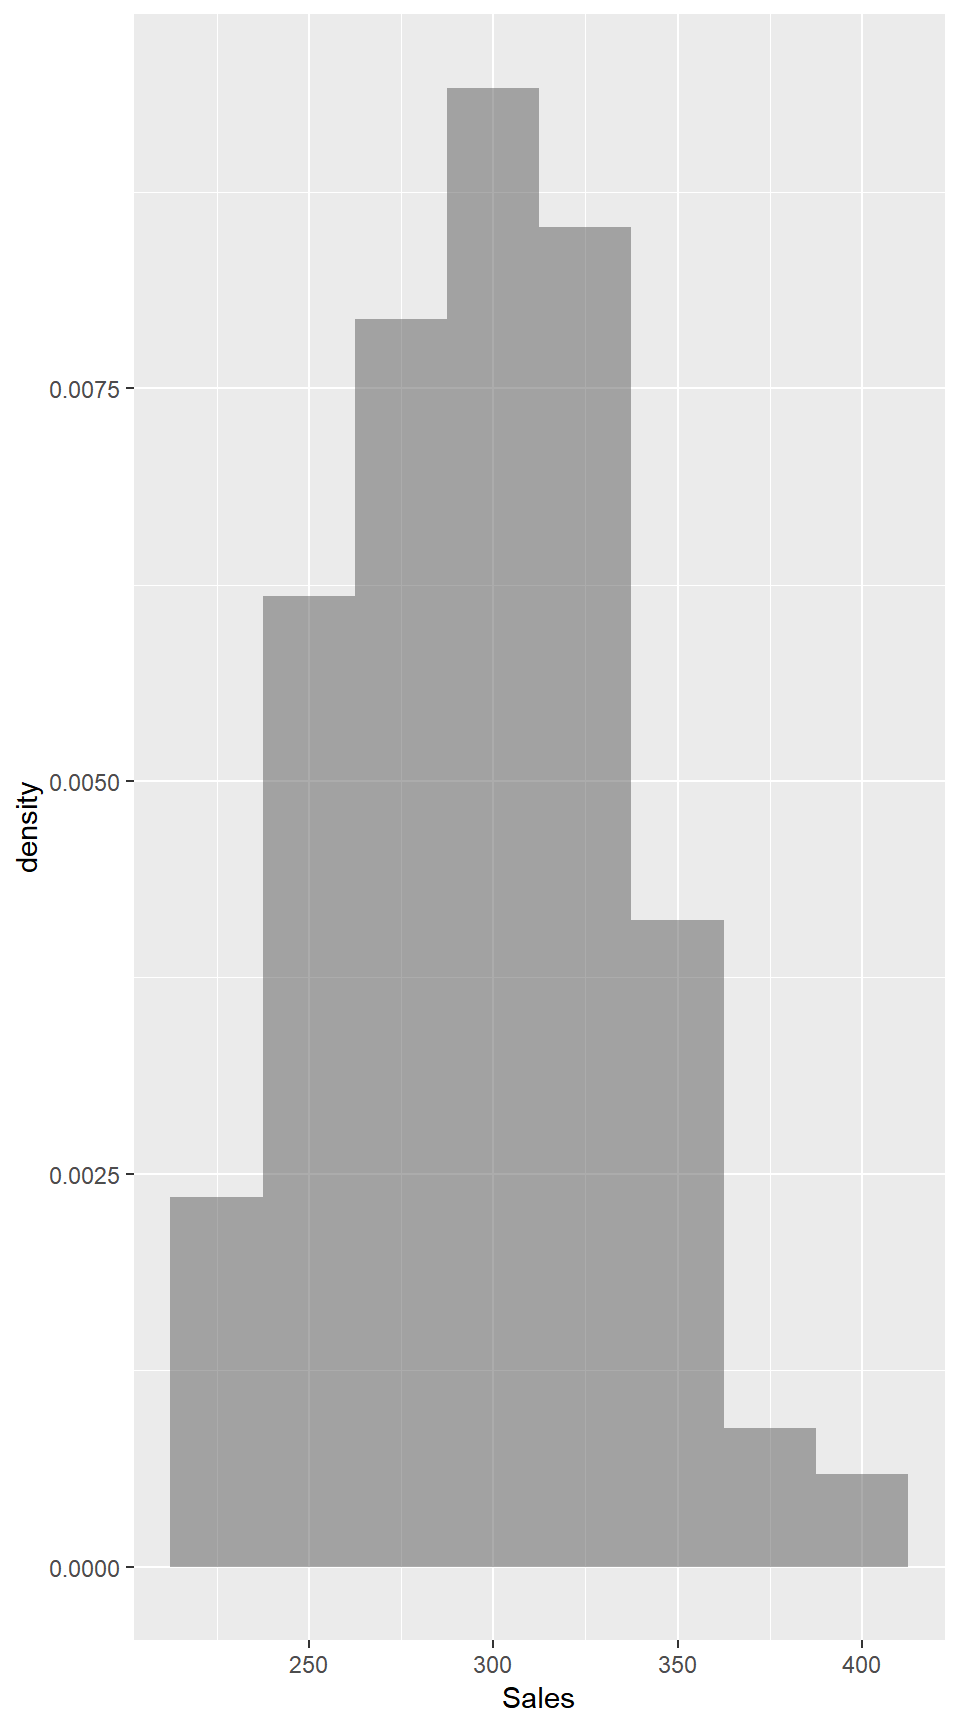
\includegraphics[width=0.65\linewidth]{Lock5WithR_files/figure-latex/Figure2.20-1}

\hypertarget{example-2.18}{%
\subsubsection{Example 2.18}\label{example-2.18}}

\begin{Shaded}
\begin{Highlighting}[]
\NormalTok{mean <-}\StringTok{ }\KeywordTok{mean}\NormalTok{( }\OperatorTok{~}\StringTok{ }\NormalTok{Sales, }\DataTypeTok{data =}\NormalTok{ RetailSales); mean}
\end{Highlighting}
\end{Shaded}

\begin{verbatim}
## [1] 296.4382
\end{verbatim}

\begin{Shaded}
\begin{Highlighting}[]
\NormalTok{sd <-}\StringTok{ }\KeywordTok{sd}\NormalTok{( }\OperatorTok{~}\StringTok{ }\NormalTok{Sales, }\DataTypeTok{data =}\NormalTok{ RetailSales); sd}
\end{Highlighting}
\end{Shaded}

\begin{verbatim}
## [1] 37.97074
\end{verbatim}

\begin{Shaded}
\begin{Highlighting}[]
\NormalTok{mean }\OperatorTok{-}\StringTok{ }\DecValTok{2}\OperatorTok{*}\NormalTok{sd}
\end{Highlighting}
\end{Shaded}

\begin{verbatim}
## [1] 220.4968
\end{verbatim}

\begin{Shaded}
\begin{Highlighting}[]
\NormalTok{mean }\OperatorTok{+}\StringTok{ }\DecValTok{2}\OperatorTok{*}\NormalTok{sd}
\end{Highlighting}
\end{Shaded}

\begin{verbatim}
## [1] 372.3797
\end{verbatim}

\hypertarget{example-2.19}{%
\subsubsection{Example 2.19}\label{example-2.19}}

Z-scores can be computed as follows:

\begin{Shaded}
\begin{Highlighting}[]
\NormalTok{( }\DecValTok{204} \OperatorTok{-}\StringTok{ }\KeywordTok{mean}\NormalTok{( }\OperatorTok{~}\StringTok{ }\NormalTok{Systolic, }\DataTypeTok{data =}\NormalTok{ ICUAdmissions) ) }\OperatorTok{/}\StringTok{ }\KeywordTok{sd}\NormalTok{( }\OperatorTok{~}\StringTok{ }\NormalTok{Systolic, }\DataTypeTok{data =}\NormalTok{ ICUAdmissions)}
\end{Highlighting}
\end{Shaded}

\begin{verbatim}
## [1] 2.176493
\end{verbatim}

\begin{Shaded}
\begin{Highlighting}[]
\NormalTok{( }\DecValTok{52} \OperatorTok{-}\StringTok{ }\KeywordTok{mean}\NormalTok{( }\OperatorTok{~}\StringTok{ }\NormalTok{HeartRate, }\DataTypeTok{data =}\NormalTok{ ICUAdmissions) ) }\OperatorTok{/}\StringTok{ }\KeywordTok{sd}\NormalTok{( }\OperatorTok{~}\StringTok{ }\NormalTok{HeartRate, }\DataTypeTok{data =}\NormalTok{ ICUAdmissions)}
\end{Highlighting}
\end{Shaded}

\begin{verbatim}
## [1] -1.749
\end{verbatim}

\hypertarget{percentiles}{%
\subsection{Percentiles}\label{percentiles}}

\hypertarget{figure-2.21}{%
\subsubsection{Figure 2.21}\label{figure-2.21}}

\begin{Shaded}
\begin{Highlighting}[]
\KeywordTok{gf_histogram}\NormalTok{( }\OperatorTok{~}\StringTok{ }\NormalTok{Close, }\DataTypeTok{binwidth =} \DecValTok{25}\NormalTok{, }\DataTypeTok{data =}\NormalTok{ SandP500)}
\end{Highlighting}
\end{Shaded}

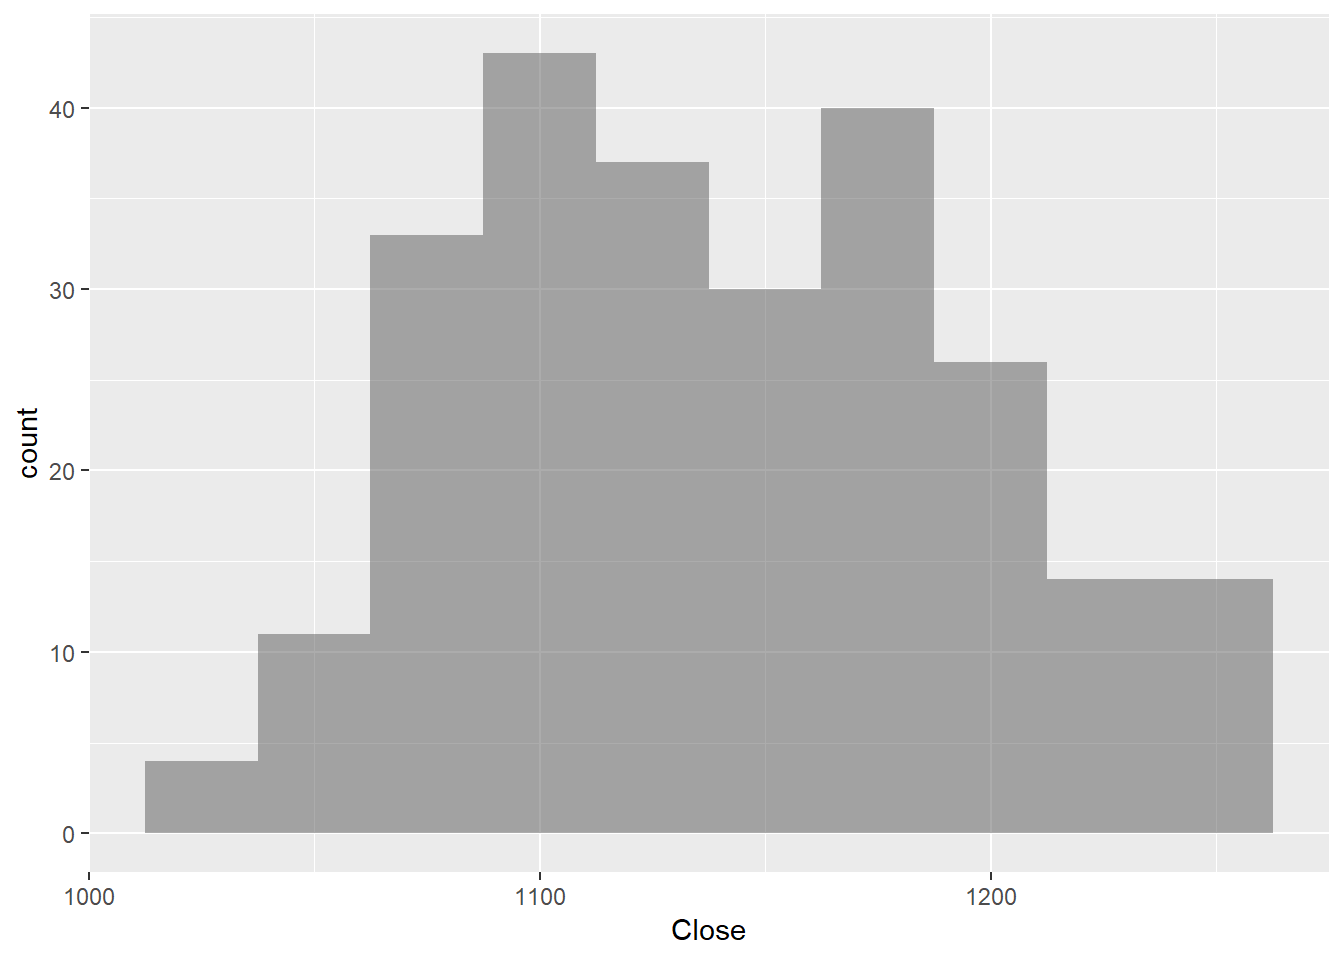
\includegraphics[width=0.65\linewidth]{Lock5WithR_files/figure-latex/Figure2.21-1}

\hypertarget{example-2.20}{%
\subsubsection{Example 2.20}\label{example-2.20}}

The text uses a histogram to estimate the \textbf{percentile} of the daily closing price for the
S\&P 500 but we can also find the exact percentiles using the \texttt{quantile()()} function.

\begin{Shaded}
\begin{Highlighting}[]
\KeywordTok{quantile}\NormalTok{(SandP500}\OperatorTok{$}\NormalTok{Close, }\DataTypeTok{probs =} \KeywordTok{seq}\NormalTok{(}\DecValTok{0}\NormalTok{, }\DecValTok{1}\NormalTok{, }\FloatTok{0.25}\NormalTok{))}
\end{Highlighting}
\end{Shaded}

\begin{verbatim}
##       0%      25%      50%      75%     100% 
## 1022.580 1094.802 1136.985 1183.372 1259.780
\end{verbatim}

\begin{Shaded}
\begin{Highlighting}[]
\KeywordTok{quantile}\NormalTok{(SandP500}\OperatorTok{$}\NormalTok{Close, }\DataTypeTok{probs =} \KeywordTok{seq}\NormalTok{(}\DecValTok{0}\NormalTok{, }\DecValTok{1}\NormalTok{, }\FloatTok{0.90}\NormalTok{))}
\end{Highlighting}
\end{Shaded}

\begin{verbatim}
##       0%      90% 
## 1022.580 1216.906
\end{verbatim}

\hypertarget{five-number-summary}{%
\subsection{Five Number Summary}\label{five-number-summary}}

We have already covered many different functions which results in the \textbf{five number summary} but \texttt{fivenum()()} is most direct way to obtain in the five number summary.

\hypertarget{example-2.21}{%
\subsubsection{Example 2.21}\label{example-2.21}}

\begin{Shaded}
\begin{Highlighting}[]
\KeywordTok{fivenum}\NormalTok{( }\OperatorTok{~}\StringTok{ }\NormalTok{Exercise, }\DataTypeTok{data =}\NormalTok{ StudentSurvey)}
\end{Highlighting}
\end{Shaded}

\hypertarget{example-2.22}{%
\subsubsection{Example 2.22}\label{example-2.22}}

\begin{Shaded}
\begin{Highlighting}[]
\KeywordTok{fivenum}\NormalTok{( }\OperatorTok{~}\StringTok{ }\NormalTok{Longevity, }\DataTypeTok{data =}\NormalTok{ MammalLongevity)}
\end{Highlighting}
\end{Shaded}

\begin{verbatim}
## [1]  1.0  8.0 12.0 15.5 40.0
\end{verbatim}

\begin{Shaded}
\begin{Highlighting}[]
\KeywordTok{min}\NormalTok{( }\OperatorTok{~}\StringTok{ }\NormalTok{Longevity, }\DataTypeTok{data =}\NormalTok{ MammalLongevity) }
\end{Highlighting}
\end{Shaded}

\begin{verbatim}
## [1] 1
\end{verbatim}

\begin{Shaded}
\begin{Highlighting}[]
\KeywordTok{max}\NormalTok{( }\OperatorTok{~}\StringTok{ }\NormalTok{Longevity, }\DataTypeTok{data =}\NormalTok{ MammalLongevity) }
\end{Highlighting}
\end{Shaded}

\begin{verbatim}
## [1] 40
\end{verbatim}

\begin{Shaded}
\begin{Highlighting}[]
\KeywordTok{range}\NormalTok{( }\OperatorTok{~}\StringTok{ }\NormalTok{Longevity, }\DataTypeTok{data =}\NormalTok{ MammalLongevity)  }\CommentTok{# subtract to get the numerical range value}
\end{Highlighting}
\end{Shaded}

\begin{verbatim}
## [1]  1 40
\end{verbatim}

\begin{Shaded}
\begin{Highlighting}[]
\KeywordTok{iqr}\NormalTok{( }\OperatorTok{~}\StringTok{ }\NormalTok{Longevity, }\DataTypeTok{data =}\NormalTok{ MammalLongevity)   }\CommentTok{# interquartile range }
\end{Highlighting}
\end{Shaded}

\begin{verbatim}
## [1] 7.25
\end{verbatim}

Note the difference in the quartile and IQR from the textbook. This results because there are several different methods to determine the quartile.

\hypertarget{example-2.23}{%
\subsubsection{Example 2.23}\label{example-2.23}}

\begin{Shaded}
\begin{Highlighting}[]
\KeywordTok{fivenum}\NormalTok{( }\OperatorTok{~}\StringTok{ }\NormalTok{DesMoines, }\DataTypeTok{data =}\NormalTok{ April14Temps)}
\end{Highlighting}
\end{Shaded}

\begin{verbatim}
## [1] 37.20 44.40 54.50 61.95 74.90
\end{verbatim}

\begin{Shaded}
\begin{Highlighting}[]
\KeywordTok{fivenum}\NormalTok{( }\OperatorTok{~}\StringTok{ }\NormalTok{SanFrancisco, }\DataTypeTok{data =}\NormalTok{ April14Temps)}
\end{Highlighting}
\end{Shaded}

\begin{verbatim}
## [1] 48.7 51.2 54.0 56.0 61.0
\end{verbatim}

\begin{Shaded}
\begin{Highlighting}[]
\KeywordTok{range}\NormalTok{( }\OperatorTok{~}\StringTok{ }\NormalTok{DesMoines, }\DataTypeTok{data =}\NormalTok{ April14Temps)}
\end{Highlighting}
\end{Shaded}

\begin{verbatim}
## [1] 37.2 74.9
\end{verbatim}

\begin{Shaded}
\begin{Highlighting}[]
\KeywordTok{diff}\NormalTok{(}\KeywordTok{range}\NormalTok{( }\OperatorTok{~}\StringTok{ }\NormalTok{DesMoines, }\DataTypeTok{data =}\NormalTok{ April14Temps))}
\end{Highlighting}
\end{Shaded}

\begin{verbatim}
## [1] 37.7
\end{verbatim}

\begin{Shaded}
\begin{Highlighting}[]
\KeywordTok{range}\NormalTok{( }\OperatorTok{~}\StringTok{ }\NormalTok{SanFrancisco, }\DataTypeTok{data =}\NormalTok{ April14Temps)}
\end{Highlighting}
\end{Shaded}

\begin{verbatim}
## [1] 48.7 61.0
\end{verbatim}

\begin{Shaded}
\begin{Highlighting}[]
\KeywordTok{diff}\NormalTok{(}\KeywordTok{range}\NormalTok{( }\OperatorTok{~}\StringTok{ }\NormalTok{SanFrancisco, }\DataTypeTok{data =}\NormalTok{ April14Temps))}
\end{Highlighting}
\end{Shaded}

\begin{verbatim}
## [1] 12.3
\end{verbatim}

\begin{Shaded}
\begin{Highlighting}[]
\KeywordTok{iqr}\NormalTok{( }\OperatorTok{~}\StringTok{ }\NormalTok{DesMoines, }\DataTypeTok{data =}\NormalTok{ April14Temps)}
\end{Highlighting}
\end{Shaded}

\begin{verbatim}
## [1] 16.875
\end{verbatim}

\begin{Shaded}
\begin{Highlighting}[]
\KeywordTok{iqr}\NormalTok{( }\OperatorTok{~}\StringTok{ }\NormalTok{SanFrancisco, }\DataTypeTok{data =}\NormalTok{ April14Temps)}
\end{Highlighting}
\end{Shaded}

\begin{verbatim}
## [1] 4.6
\end{verbatim}

\hypertarget{outliers-boxplots-and-quantitativecategorical-relationships}{%
\section{Outliers, Boxplots, and Quantitative/Categorical Relationships}\label{outliers-boxplots-and-quantitativecategorical-relationships}}

\hypertarget{detection-of-outliers}{%
\subsection{Detection of Outliers}\label{detection-of-outliers}}

Generally, outliers are considered to be values

\begin{enumerate}
\tightlist
\item
  less than \(Q_1 - 1.5 TEX COMMAND NOT FOUND cdot (IQR)\), and
\item
  greater than \(Q_3 + 1.5 TEX COMMAND NOT FOUND cdot (IQR)\).\\
\end{enumerate}

\hypertarget{example-2.25}{%
\subsubsection{Example 2.25}\label{example-2.25}}

\begin{Shaded}
\begin{Highlighting}[]
\KeywordTok{fivenum}\NormalTok{( }\OperatorTok{~}\StringTok{ }\NormalTok{Longevity, }\DataTypeTok{data =}\NormalTok{ MammalLongevity)}
\end{Highlighting}
\end{Shaded}

\begin{verbatim}
## [1]  1.0  8.0 12.0 15.5 40.0
\end{verbatim}

\begin{Shaded}
\begin{Highlighting}[]
\KeywordTok{iqr}\NormalTok{( }\OperatorTok{~}\StringTok{ }\NormalTok{Longevity, }\DataTypeTok{data =}\NormalTok{ MammalLongevity)}
\end{Highlighting}
\end{Shaded}

\begin{verbatim}
## [1] 7.25
\end{verbatim}

\begin{Shaded}
\begin{Highlighting}[]
\FloatTok{8.0-1.5}\OperatorTok{*}\FloatTok{7.25}
\end{Highlighting}
\end{Shaded}

\begin{verbatim}
## [1] -2.875
\end{verbatim}

\begin{Shaded}
\begin{Highlighting}[]
\FloatTok{15.5+1.5}\OperatorTok{*}\FloatTok{7.25}
\end{Highlighting}
\end{Shaded}

\begin{verbatim}
## [1] 26.375
\end{verbatim}

\begin{Shaded}
\begin{Highlighting}[]
\KeywordTok{subset}\NormalTok{(MammalLongevity, Longevity}\OperatorTok{>}\FloatTok{26.375}\NormalTok{)}
\end{Highlighting}
\end{Shaded}

\begin{verbatim}
##      Animal Gestation Longevity
## 15 elephant       645        40
\end{verbatim}

There is no function in R that directly results in outliers because practically, there is no one specific formula for such a determination. However, a boxplot will indirectly reveal outliers.

\hypertarget{boxplots}{%
\subsection{Boxplots}\label{boxplots}}

A way to visualize the five number summary and outliers for a variable is to create a boxplot.

\hypertarget{example-2.26}{%
\subsubsection{Example 2.26}\label{example-2.26}}

\begin{Shaded}
\begin{Highlighting}[]
\KeywordTok{favstats}\NormalTok{( }\OperatorTok{~}\StringTok{ }\NormalTok{Longevity, }\DataTypeTok{data =}\NormalTok{ MammalLongevity)}
\end{Highlighting}
\end{Shaded}

\begin{verbatim}
##  min Q1 median    Q3 max  mean       sd  n missing
##    1  8     12 15.25  40 13.15 7.244981 40       0
\end{verbatim}

\begin{Shaded}
\begin{Highlighting}[]
\KeywordTok{gf_boxplot}\NormalTok{(Longevity }\OperatorTok{~}\StringTok{ ", xlab = "}\NormalTok{, }\DataTypeTok{data =}\NormalTok{ MammalLongevity) }\OperatorTok
\StringTok{  }\KeywordTok{gf_refine}\NormalTok{(}\KeywordTok{coord_flip}\NormalTok{())}
\end{Highlighting}
\end{Shaded}

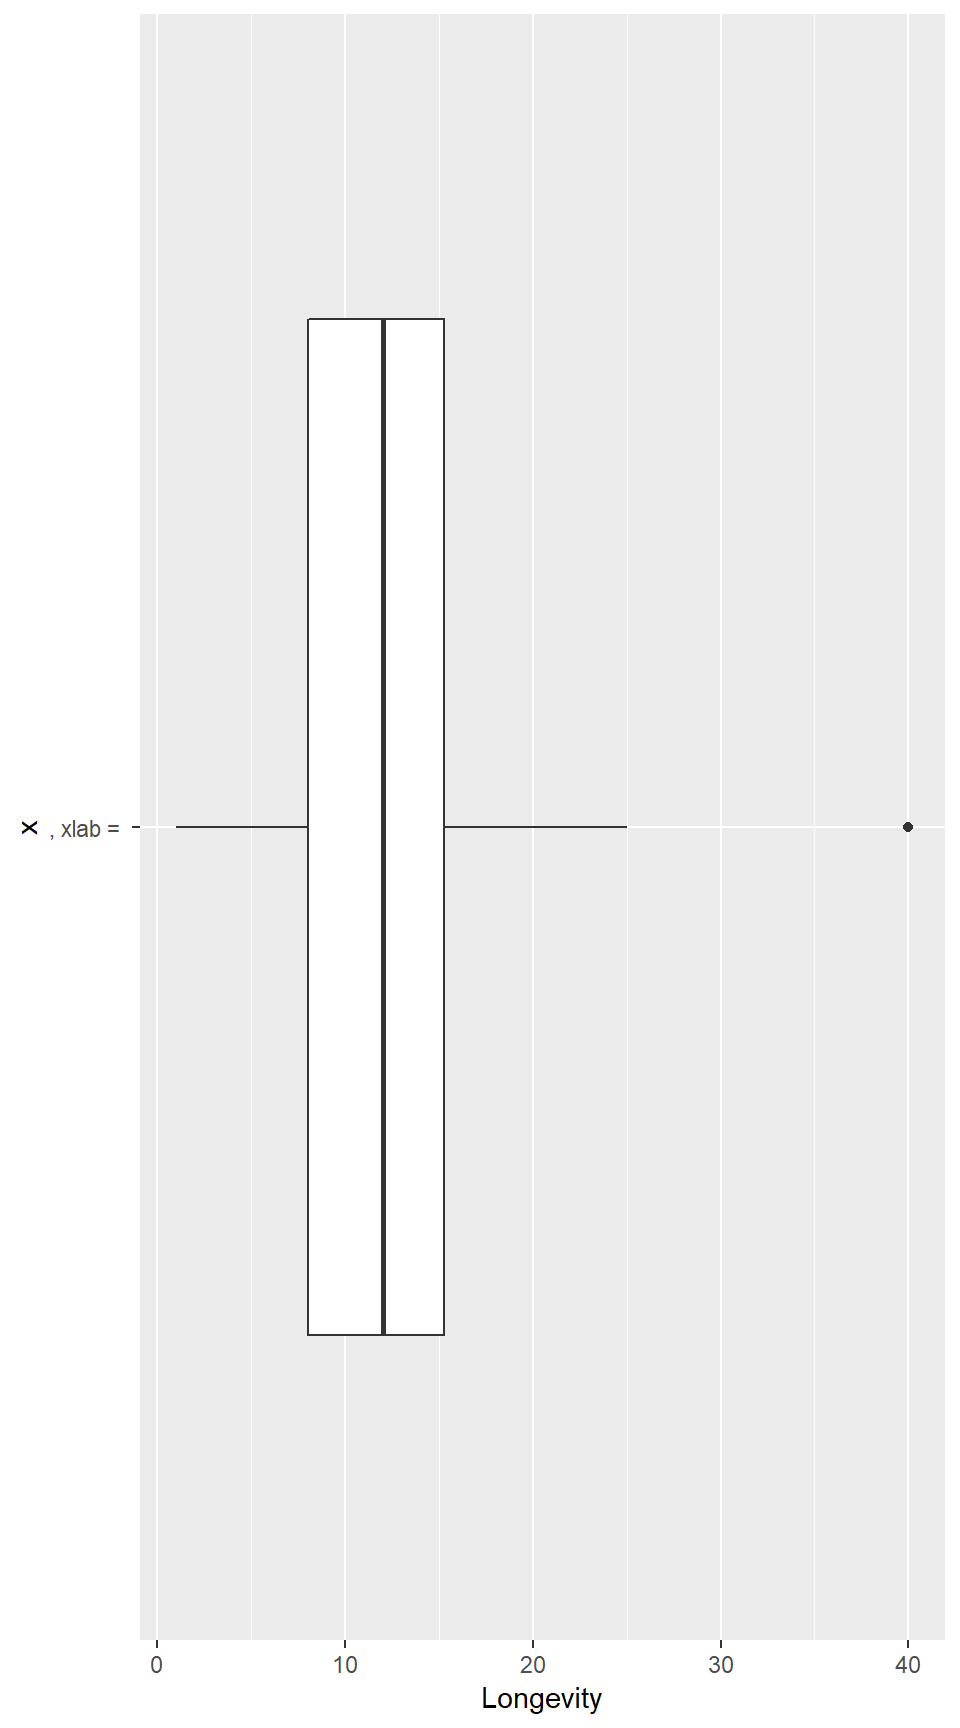
\includegraphics[width=0.65\linewidth]{Lock5WithR_files/figure-latex/Example2.26-1}

\hypertarget{figure-2.32}{%
\subsubsection{Figure 2.32}\label{figure-2.32}}

\begin{Shaded}
\begin{Highlighting}[]
\KeywordTok{gf_boxplot}\NormalTok{(Smokers }\OperatorTok{~}\StringTok{ ", xlab = "}\NormalTok{, }\DataTypeTok{data =}\NormalTok{ USStates) }\OperatorTok
\StringTok{  }\KeywordTok{gf_refine}\NormalTok{(}\KeywordTok{coord_flip}\NormalTok{())}
\end{Highlighting}
\end{Shaded}

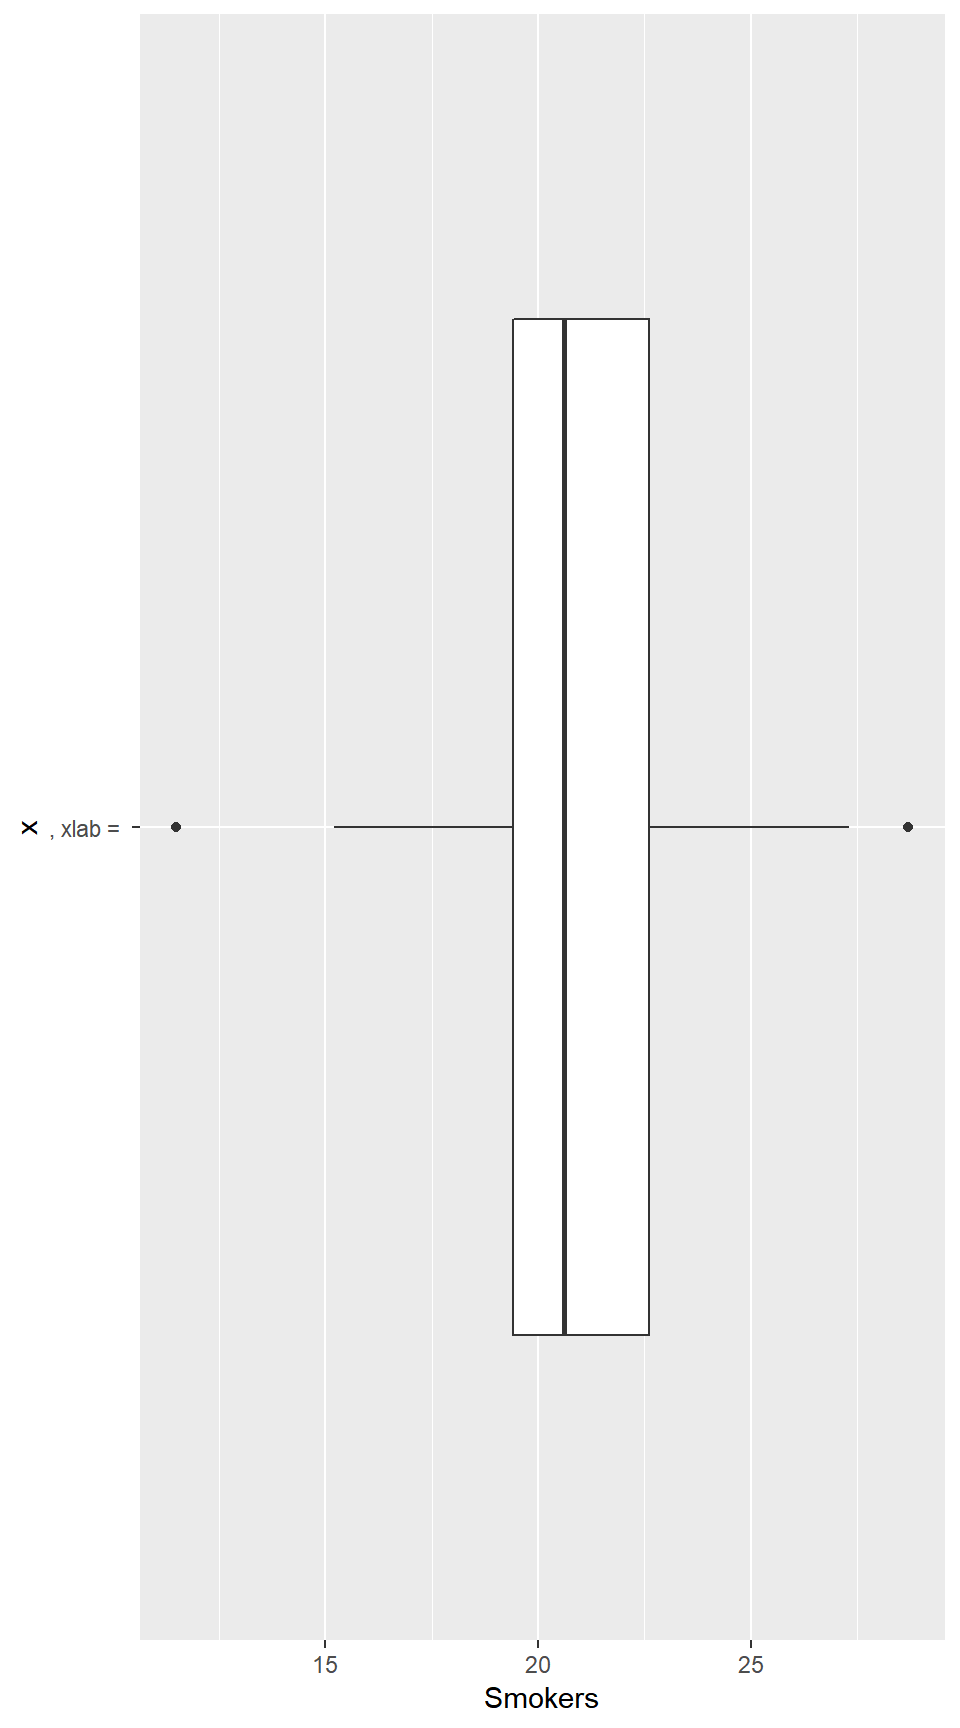
\includegraphics[width=0.65\linewidth]{Lock5WithR_files/figure-latex/Figure2.32-1}

\hypertarget{example-2.27}{%
\subsubsection{Example 2.27}\label{example-2.27}}

We can similarity investigate the \emph{Smokers} variable in {USStates}.

\begin{Shaded}
\begin{Highlighting}[]
\KeywordTok{fivenum}\NormalTok{( }\OperatorTok{~}\StringTok{ }\NormalTok{Smokers, }\DataTypeTok{data =}\NormalTok{ USStates)}
\end{Highlighting}
\end{Shaded}

\begin{verbatim}
## [1] 11.5 19.3 20.6 22.6 28.7
\end{verbatim}

The boxplot reveals two outliers. To identify them, we can again use \texttt{subset()()} for smokers greater or less than the \emph{whiskers} of the boxplot.

\begin{Shaded}
\begin{Highlighting}[]
\KeywordTok{subset}\NormalTok{(USStates, Smokers}\OperatorTok{<}\DecValTok{15}\NormalTok{)}
\end{Highlighting}
\end{Shaded}

\begin{verbatim}
##    State HouseholdIncome    IQ McCainVote Region ObamaMcCain Population
## 44  Utah           55619 101.1      0.629      W           M   2.420708
##    EighthGradeMath HighSchool   GSP FiveVegetables Smokers
## 44          279.16         91 36758           22.1    11.5
##    PhysicalActivity Obese College NonWhite HeavyDrinkers Pres2008
## 44             83.1  21.2      31     12.1           2.9   McCain
\end{verbatim}

\begin{Shaded}
\begin{Highlighting}[]
\KeywordTok{subset}\NormalTok{(USStates, Smokers}\OperatorTok{>}\DecValTok{28}\NormalTok{)}
\end{Highlighting}
\end{Shaded}

\begin{verbatim}
##       State HouseholdIncome   IQ McCainVote Region ObamaMcCain Population
## 17 Kentucky           38694 99.4      0.575     MW           M   4.141835
##    EighthGradeMath HighSchool   GSP FiveVegetables Smokers
## 17          273.98       81.8 33666           16.8    28.7
##    PhysicalActivity Obese College NonWhite HeavyDrinkers Pres2008
## 17             70.1  28.6    22.6      9.4           2.7   McCain
\end{verbatim}

\hypertarget{figure-2.33}{%
\subsubsection{Figure 2.33}\label{figure-2.33}}

\begin{Shaded}
\begin{Highlighting}[]
\KeywordTok{gf_boxplot}\NormalTok{(Budget }\OperatorTok{~}\StringTok{ ", xlab = "}\NormalTok{, }\DataTypeTok{data =}\NormalTok{ HollywoodMovies2011) }\OperatorTok
\StringTok{  }\KeywordTok{gf_refine}\NormalTok{(}\KeywordTok{coord_flip}\NormalTok{())}
\end{Highlighting}
\end{Shaded}

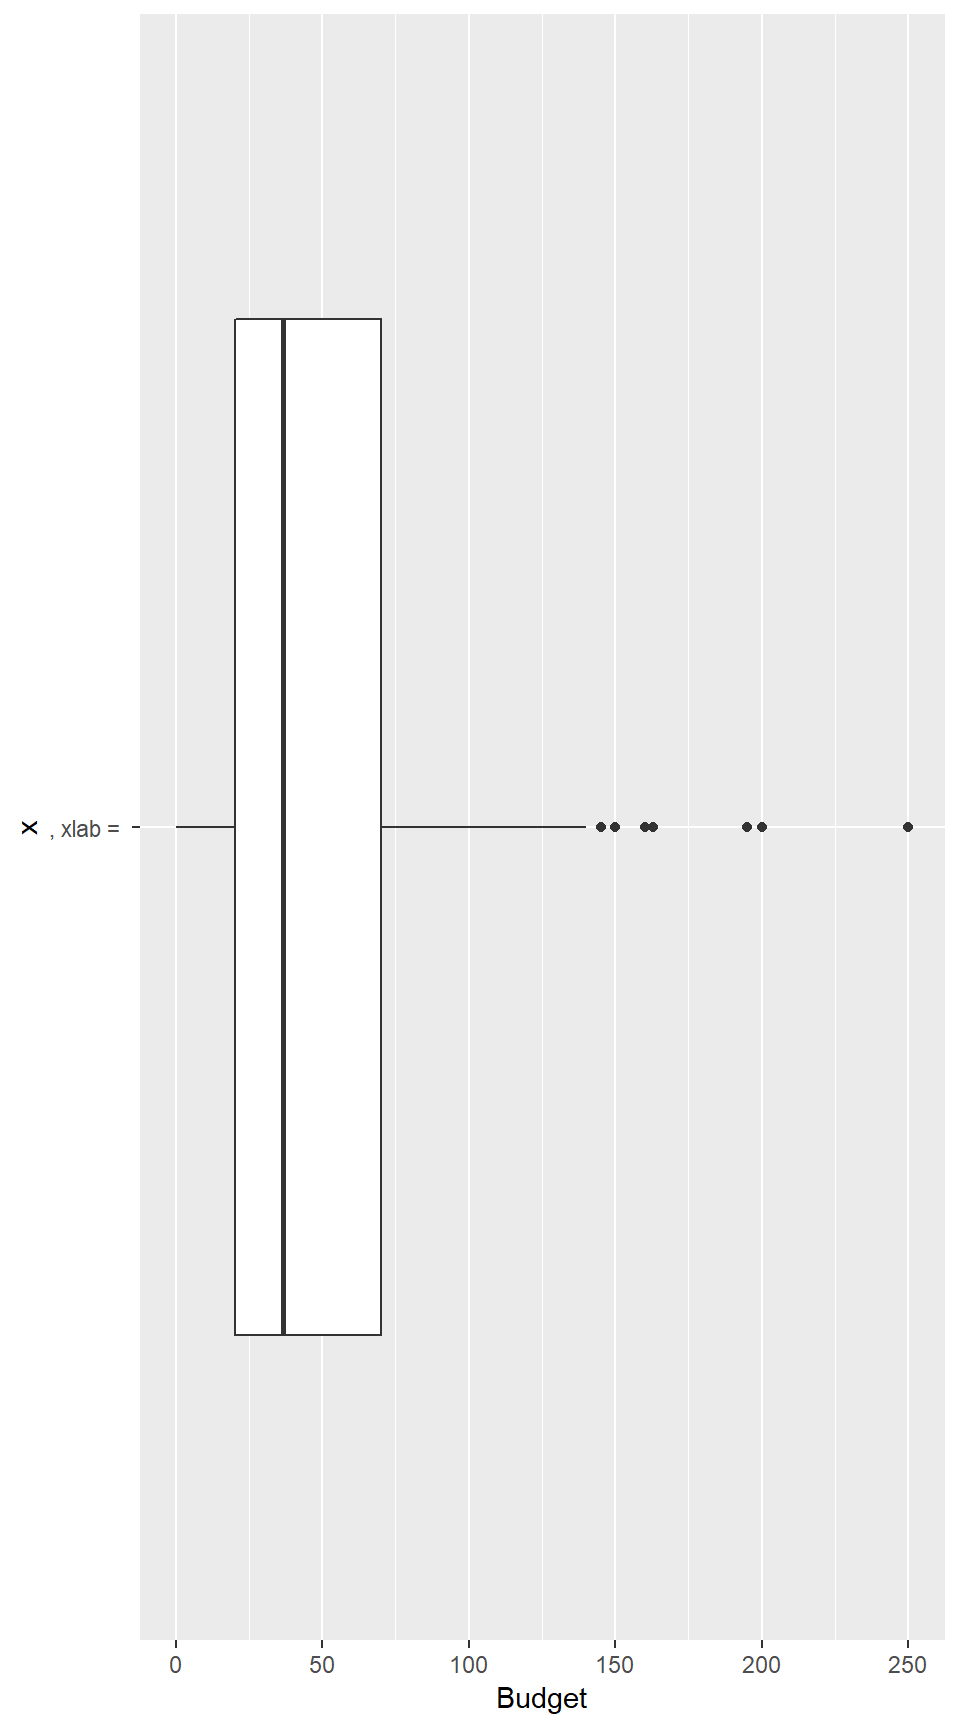
\includegraphics[width=0.65\linewidth]{Lock5WithR_files/figure-latex/Figure2.33-1}

\hypertarget{example-2.28}{%
\subsubsection{Example 2.28}\label{example-2.28}}

\begin{Shaded}
\begin{Highlighting}[]
\KeywordTok{subset}\NormalTok{(HollywoodMovies2011, Budget}\OperatorTok{>}\DecValTok{225}\NormalTok{)}
\end{Highlighting}
\end{Shaded}

\begin{verbatim}
##                                           Movie LeadStudio RottenTomatoes
## 30 Pirates of the Caribbean:\nOn Stranger Tides     Disney             34
##    AudienceScore Story  Genre TheatersOpenWeek BOAverageOpenWeek
## 30            61 Quest Action             4155             21697
##    DomesticGross ForeignGross WorldGross Budget Profitability
## 30        241.07        802.8   1043.871    250      4.175484
##    OpeningWeekend
## 30          90.15
\end{verbatim}

\begin{Shaded}
\begin{Highlighting}[]
\KeywordTok{head}\NormalTok{(HollywoodMovies2011)}
\end{Highlighting}
\end{Shaded}

\begin{verbatim}
##                                         Movie       LeadStudio
## 1                                   Insidious             Sony
## 2                       Paranormal Activity 3      Independent
## 3                                 Bad Teacher      Independent
## 4 Harry Potter and the Deathly Hallows Part 2      Warner Bros
## 5                                 Bridesmaids Relativity Media
## 6                           Midnight in Paris             Sony
##   RottenTomatoes AudienceScore         Story   Genre TheatersOpenWeek
## 1             67            65 Monster Force  Horror             2408
## 2             68            58 Monster Force  Horror             3321
## 3             44            38        Comedy  Comedy             3049
## 4             96            92       Rivalry Fantasy             4375
## 5             90            77       Rivalry  Comedy             2918
## 6             93            84          Love Romance              944
##   BOAverageOpenWeek DomesticGross ForeignGross WorldGross Budget
## 1              5511         54.01        43.00     97.009    1.5
## 2             15829        103.66        98.24    201.897    5.0
## 3             10365        100.29       115.90    216.196   20.0
## 4             38672        381.01       947.10   1328.111  125.0
## 5              8995        169.11       119.28    288.382   32.5
## 6              6177         56.18        83.00    139.177   17.0
##   Profitability OpeningWeekend
## 1     64.672667          13.27
## 2     40.379400          52.57
## 3     10.809800          31.60
## 4     10.624888         169.19
## 5      8.873292          26.25
## 6      8.186882           5.83
\end{verbatim}

\hypertarget{one-quantitative-and-one-categorical-variable}{%
\subsection{One Quantitative and One Categorical Variable}\label{one-quantitative-and-one-categorical-variable}}

The formula for a \textbf{\texttt{lattice}} plot can be extended to create multiple panels (sometimes called \textbf{facets}) based on a ``condition'', often given by another variable. This is another way to look at multiple groups simultaneously. The general syntax for this becomes

\begin{Shaded}
\begin{Highlighting}[]
\KeywordTok{plotname}\NormalTok{( }\OperatorTok{~}\StringTok{ }\NormalTok{variable }\OperatorTok{|}\StringTok{ }\NormalTok{condition, }\DataTypeTok{data =}\NormalTok{ dataName )}
\end{Highlighting}
\end{Shaded}

\hypertarget{figure-2.34}{%
\subsubsection{Figure 2.34}\label{figure-2.34}}

Depending on the type of plot, you will want to use conditioning.

\begin{Shaded}
\begin{Highlighting}[]
\KeywordTok{gf_boxplot}\NormalTok{(TV }\OperatorTok{~}\StringTok{ }\NormalTok{Gender, }\DataTypeTok{data =}\NormalTok{ StudentSurvey) }\OperatorTok
\StringTok{  }\KeywordTok{gf_refine}\NormalTok{(}\KeywordTok{coord_flip}\NormalTok{())}
\end{Highlighting}
\end{Shaded}

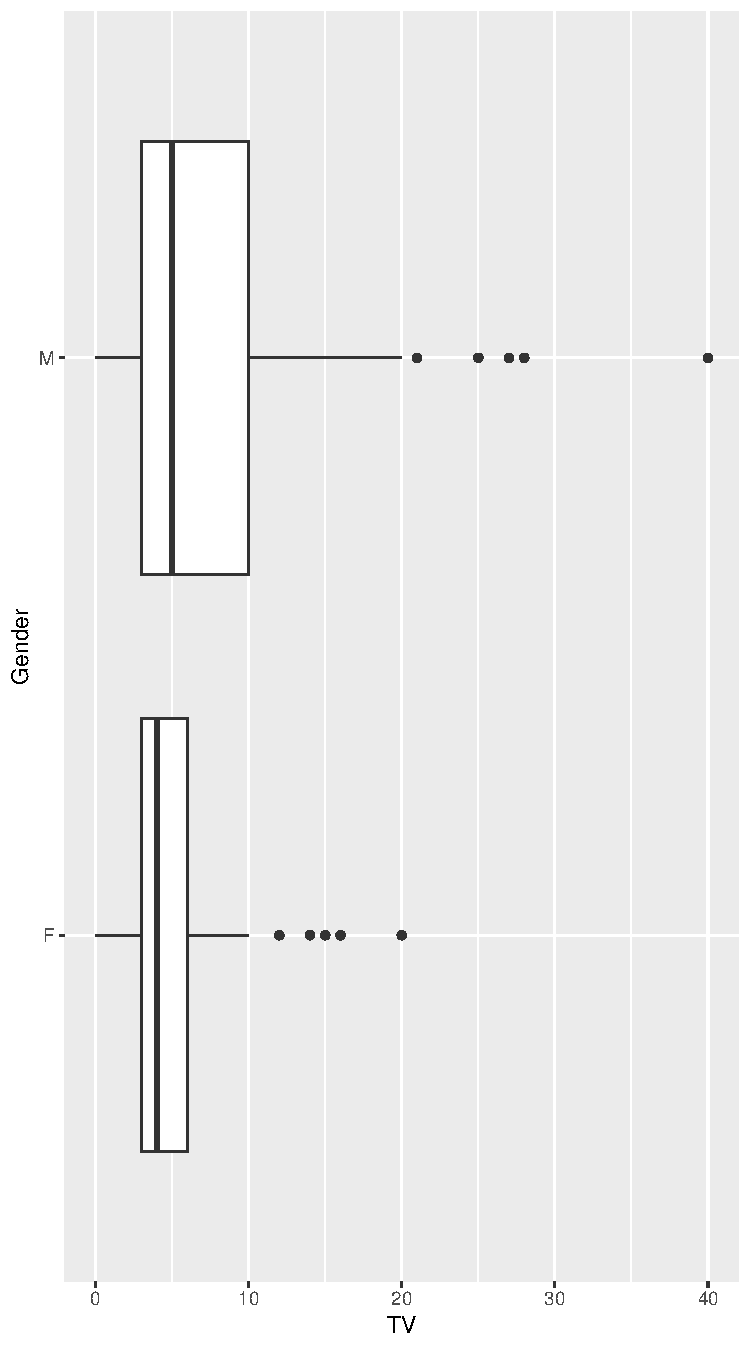
\includegraphics[width=0.65\linewidth]{Lock5WithR_files/figure-latex/Figure2.34-1}

\begin{Shaded}
\begin{Highlighting}[]
\KeywordTok{gf_dotplot}\NormalTok{( }\OperatorTok{~}\StringTok{ }\NormalTok{TV}\OperatorTok{|}\NormalTok{Gender, }\DataTypeTok{binwidth =} \DecValTok{1}\NormalTok{, }\DataTypeTok{dotsize =} \FloatTok{.35}\NormalTok{, }\DataTypeTok{data =}\NormalTok{ StudentSurvey)}
\end{Highlighting}
\end{Shaded}

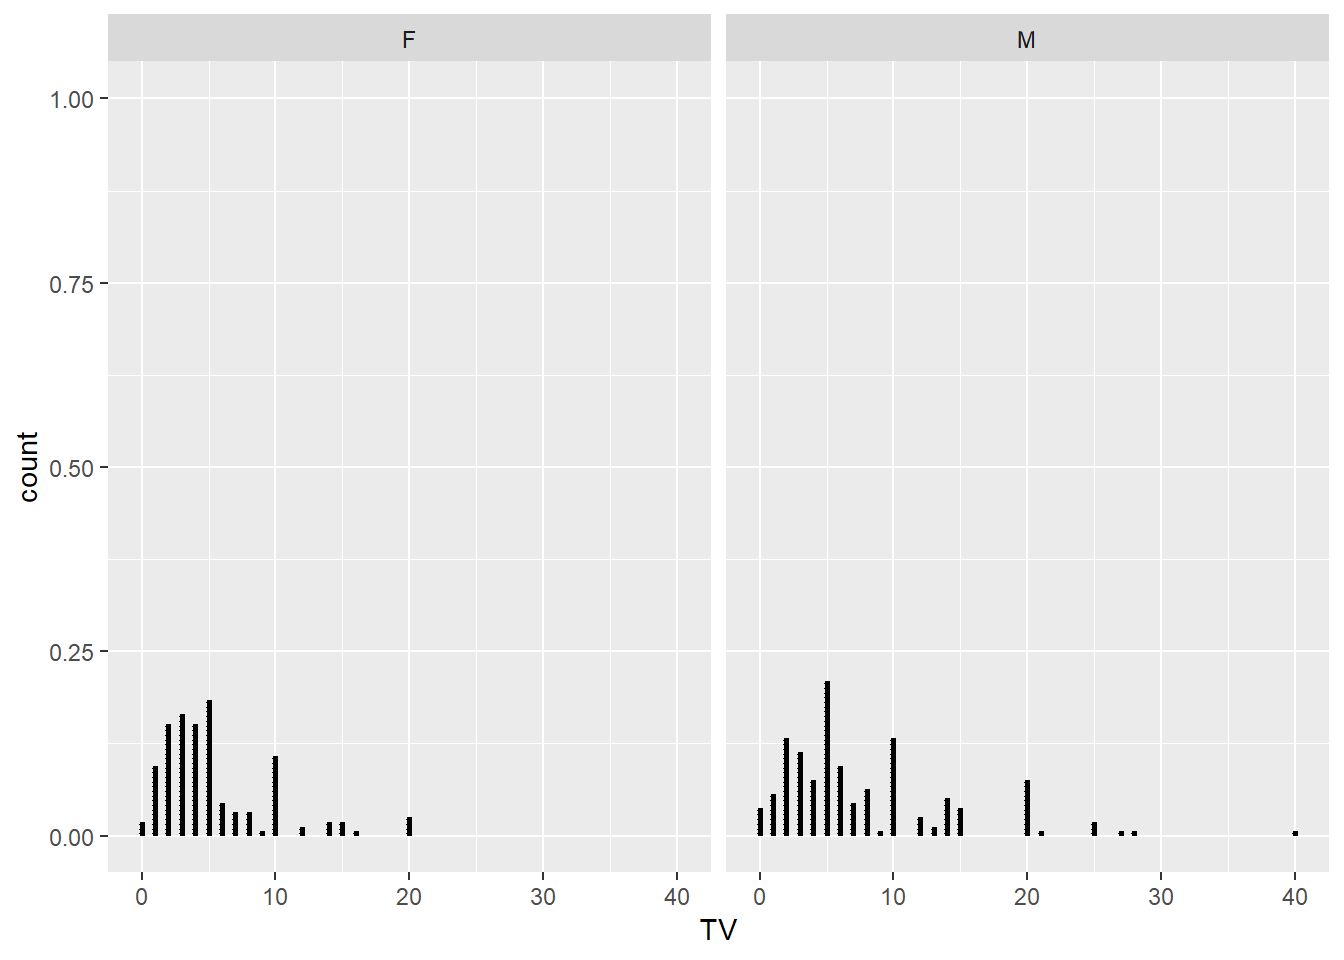
\includegraphics[width=0.65\linewidth]{Lock5WithR_files/figure-latex/Figure2.34-2}

We can do the same thing for bar graphs.

\begin{Shaded}
\begin{Highlighting}[]
\KeywordTok{gf_bar}\NormalTok{( }\OperatorTok{~}\StringTok{ }\NormalTok{Award }\OperatorTok{|}\StringTok{ }\NormalTok{Gender, }\DataTypeTok{data =}\NormalTok{ StudentSurvey)}
\end{Highlighting}
\end{Shaded}

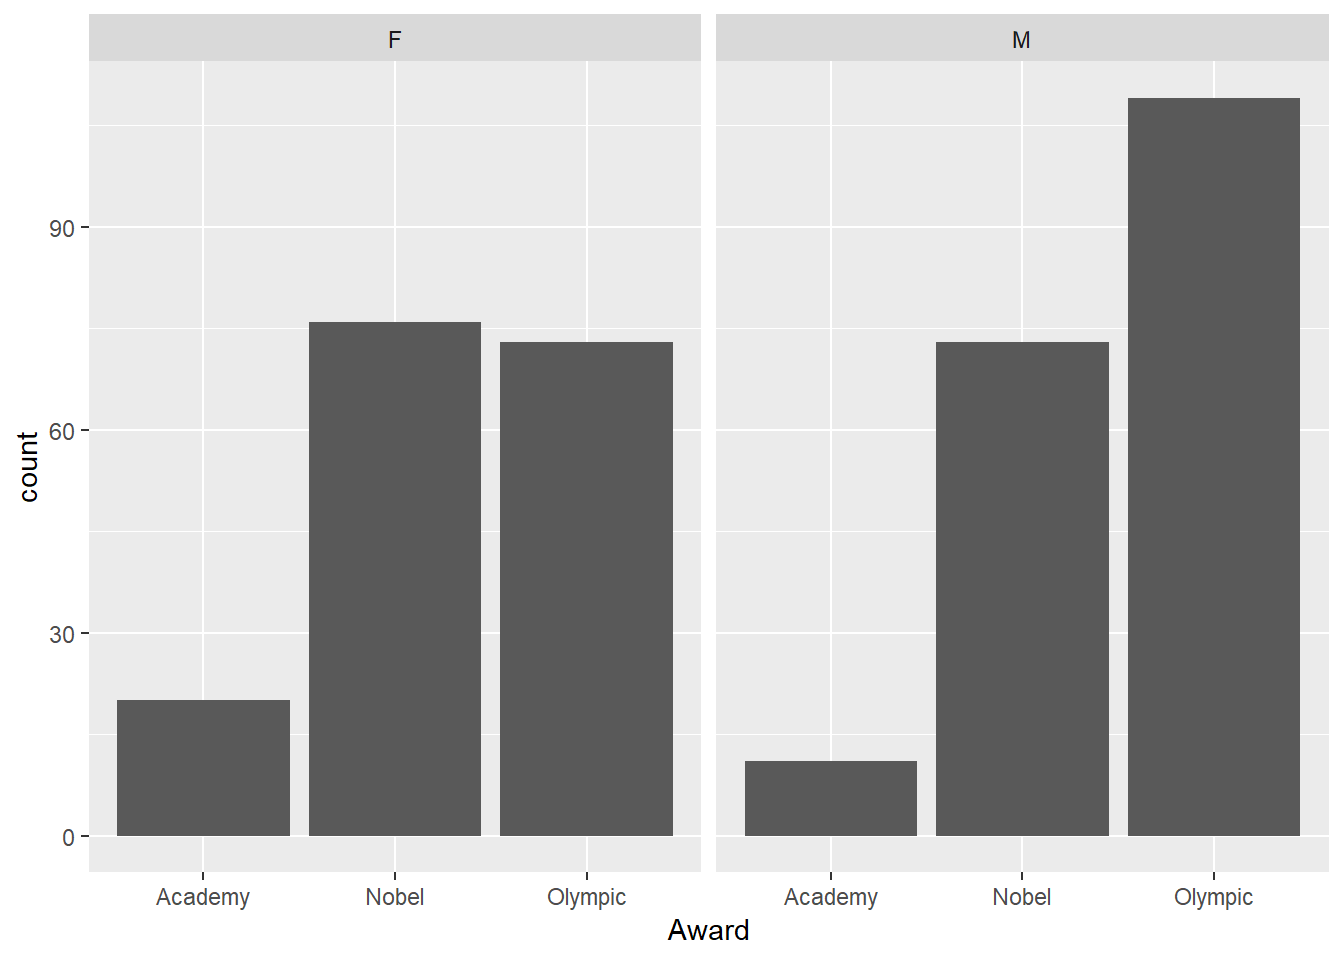
\includegraphics[width=0.65\linewidth]{Lock5WithR_files/figure-latex/Figure2.34b-1}

This graph should be familiar as we have plotted these variables together previously. Here we used different panels, but before, in 2.1, we had used grouping. Note that we can combine grouping and conditioning in the same plot.

\hypertarget{example-2.31}{%
\subsubsection{Example 2.31}\label{example-2.31}}

\begin{Shaded}
\begin{Highlighting}[]
\KeywordTok{favstats}\NormalTok{( }\OperatorTok{~}\StringTok{ }\NormalTok{TV }\OperatorTok{|}\StringTok{ }\NormalTok{Gender, }\DataTypeTok{data =}\NormalTok{ StudentSurvey)}
\KeywordTok{diffmean}\NormalTok{( }\OperatorTok{~}\StringTok{ }\NormalTok{TV }\OperatorTok{|}\StringTok{ }\NormalTok{Gender, }\DataTypeTok{data =}\NormalTok{ StudentSurvey)}
\end{Highlighting}
\end{Shaded}

\hypertarget{two-quantitative-variables-scatterplot-and-correlation}{%
\section{Two Quantitative Variables: Scatterplot and Correlation}\label{two-quantitative-variables-scatterplot-and-correlation}}

\hypertarget{example-2.32}{%
\subsubsection{Example 2.32}\label{example-2.32}}

\begin{Shaded}
\begin{Highlighting}[]
\NormalTok{ElectionMargin}
\end{Highlighting}
\end{Shaded}

\begin{verbatim}
##    Year  Candidate Approval Margin Result
## 1  1940  Roosevelt       62   10.0    Won
## 2  1948     Truman       50    4.5    Won
## 3  1956 Eisenhower       70   15.4    Won
## 4  1964    Johnson       67   22.6    Won
## 5  1972      Nixon       57   23.2    Won
## 6  1976       Ford       48   -2.1   Lost
## 7  1980     Carter       31   -9.7   Lost
## 8  1984     Reagan       57   18.2    Won
## 9  1992 G.H.W.Bush       39   -5.5   Lost
## 10 1996    Clinton       55    8.5    Won
## 11 2004   G.W.Bush       49    2.4    Won
\end{verbatim}

\hypertarget{visualizing-a-relationship-between-two-quantitative-variables-scatterplots}{%
\subsection{Visualizing a Relationship between Two Quantitative Variables: Scatterplots}\label{visualizing-a-relationship-between-two-quantitative-variables-scatterplots}}

The most common way to look at two quantitative variables is with a scatterplot. The \textbf{\texttt{ggformula}} function for this is \texttt{gf\_point()()}, and the basic syntax is

\begin{Shaded}
\begin{Highlighting}[]
\KeywordTok{gf_point}\NormalTok{(yvar }\OperatorTok{~}\StringTok{ }\NormalTok{xvar, }\DataTypeTok{data =}\NormalTok{ dataName)}
\end{Highlighting}
\end{Shaded}

Notice that now we have something on both sides of the \textasciitilde\{\} since we need to tell \R~about two variables.

\hypertarget{example-2.33}{%
\subsubsection{Example 2.33}\label{example-2.33}}

\begin{Shaded}
\begin{Highlighting}[]
\KeywordTok{gf_point}\NormalTok{(Margin }\OperatorTok{~}\StringTok{ }\NormalTok{Approval, }\DataTypeTok{data =}\NormalTok{ ElectionMargin)}
\end{Highlighting}
\end{Shaded}

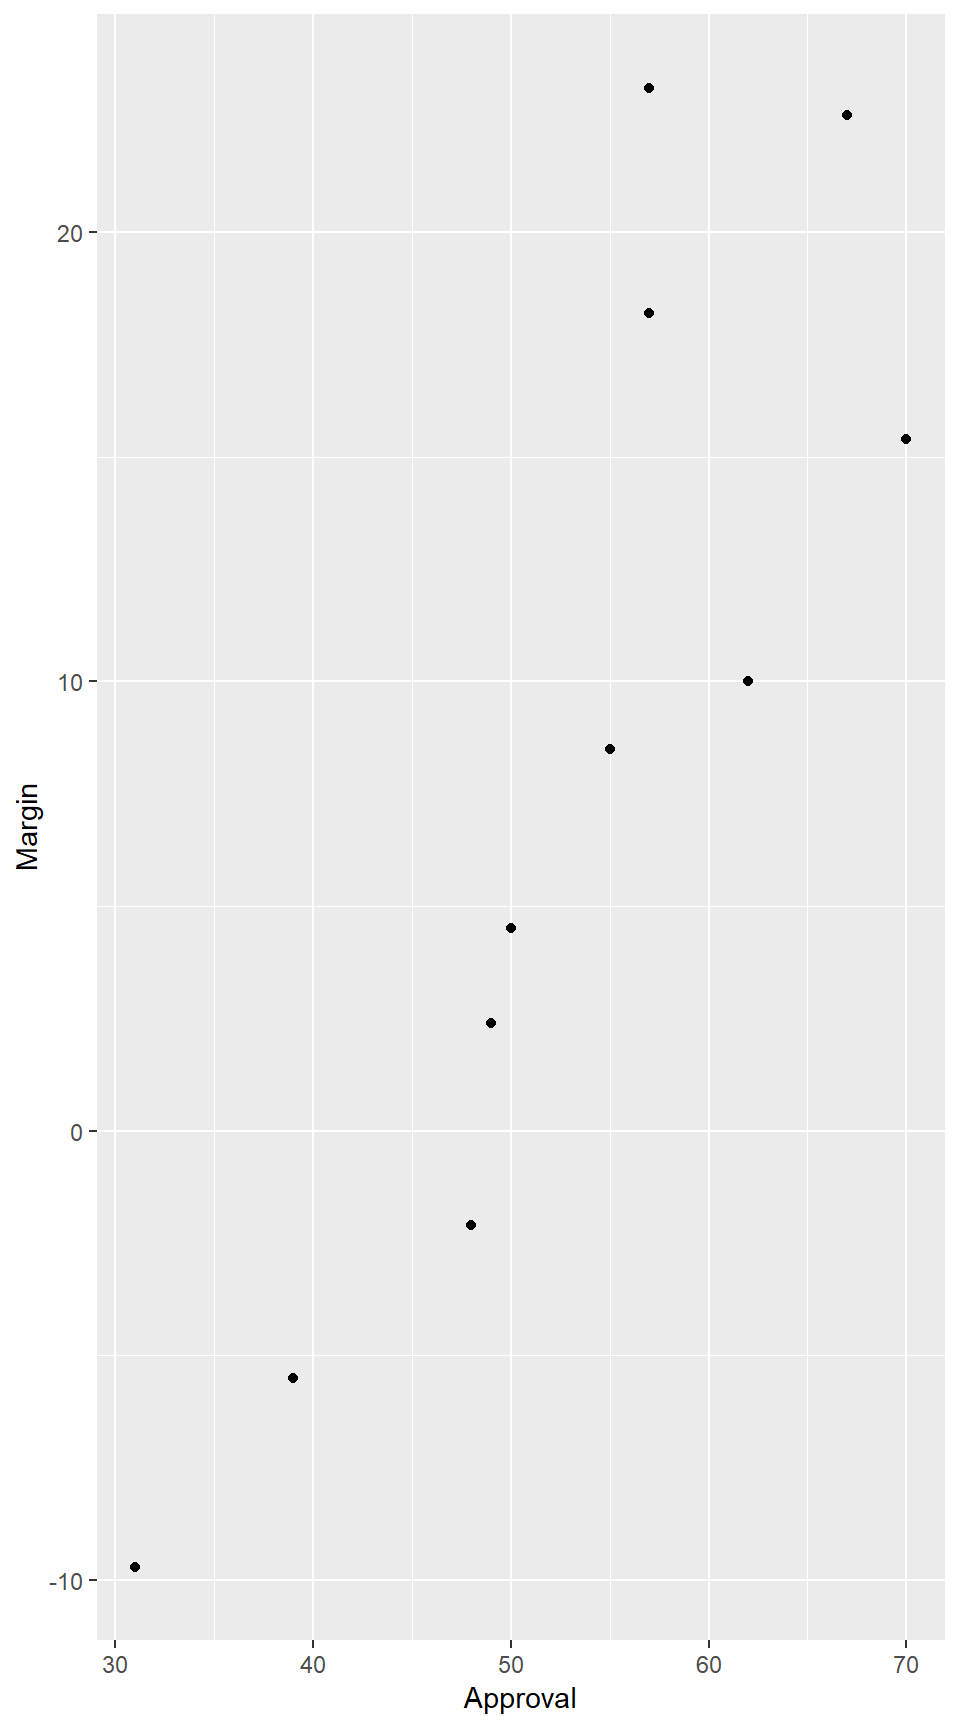
\includegraphics[width=0.65\linewidth]{Lock5WithR_files/figure-latex/Example2.33-1}

\hypertarget{figure-2.49}{%
\subsubsection{Figure 2.49}\label{figure-2.49}}

\begin{Shaded}
\begin{Highlighting}[]
\KeywordTok{gf_point}\NormalTok{(AvgMercury }\OperatorTok{~}\StringTok{ }\NormalTok{pH, }\DataTypeTok{data =}\NormalTok{ FloridaLakes)}
\end{Highlighting}
\end{Shaded}

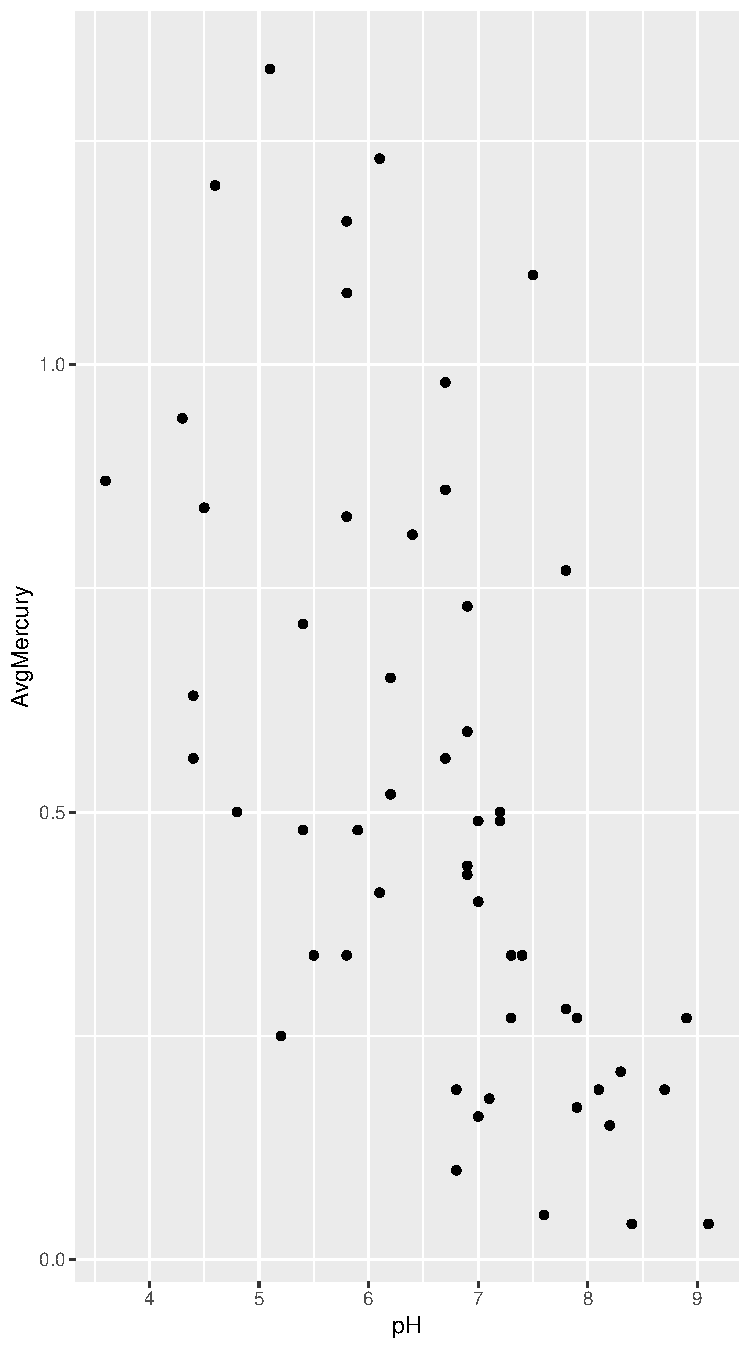
\includegraphics[width=0.65\linewidth]{Lock5WithR_files/figure-latex/Figure2.49-1}

\begin{Shaded}
\begin{Highlighting}[]
\KeywordTok{gf_point}\NormalTok{(AvgMercury }\OperatorTok{~}\StringTok{ }\NormalTok{Alkalinity, }\DataTypeTok{data =}\NormalTok{ FloridaLakes)}
\end{Highlighting}
\end{Shaded}

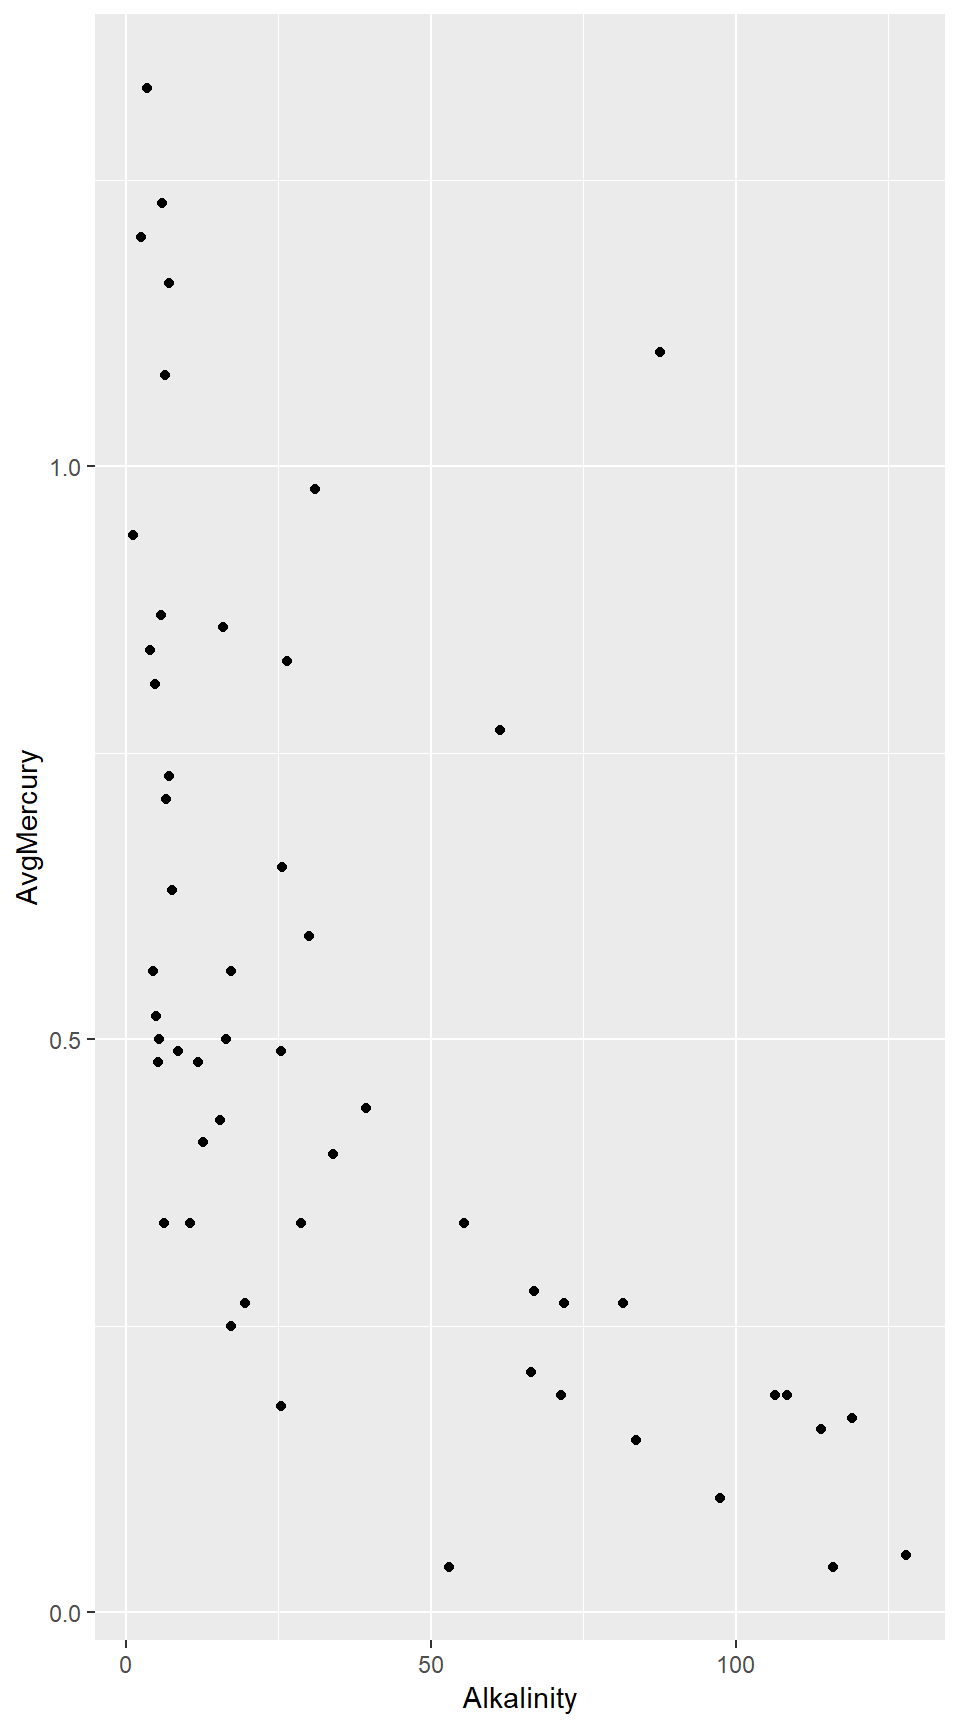
\includegraphics[width=0.65\linewidth]{Lock5WithR_files/figure-latex/Figure2.49-2}

\begin{Shaded}
\begin{Highlighting}[]
\KeywordTok{gf_point}\NormalTok{(Alkalinity }\OperatorTok{~}\StringTok{ }\NormalTok{pH, }\DataTypeTok{data =}\NormalTok{ FloridaLakes)}
\end{Highlighting}
\end{Shaded}

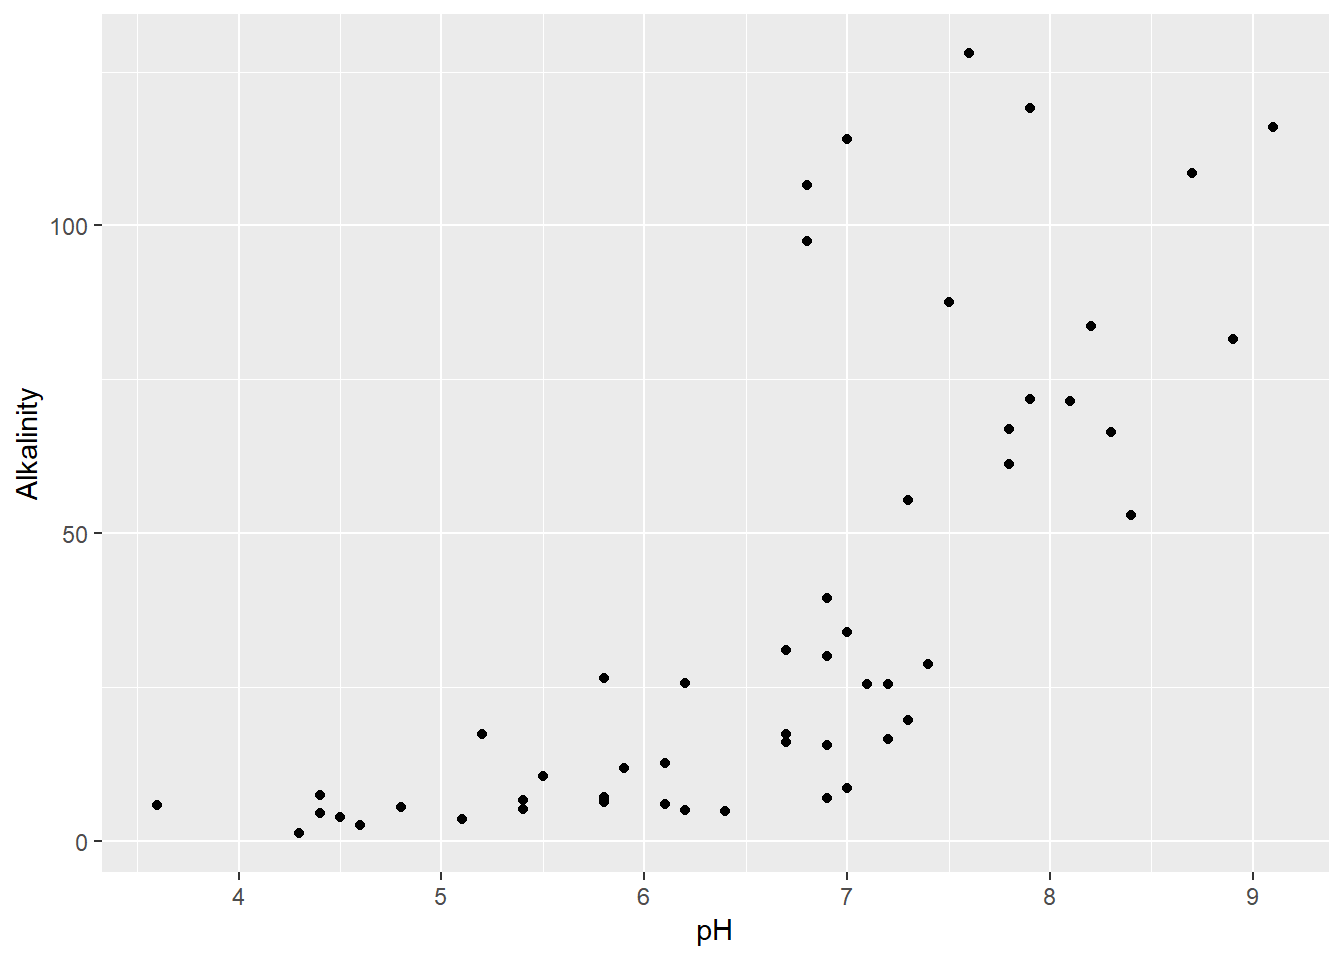
\includegraphics[width=0.65\linewidth]{Lock5WithR_files/figure-latex/Figure2.49-3}

\begin{Shaded}
\begin{Highlighting}[]
\KeywordTok{gf_point}\NormalTok{(AvgMercury }\OperatorTok{~}\StringTok{ }\NormalTok{ThreeYrStdMercury, }\DataTypeTok{data =}\NormalTok{ FloridaLakes)}
\end{Highlighting}
\end{Shaded}

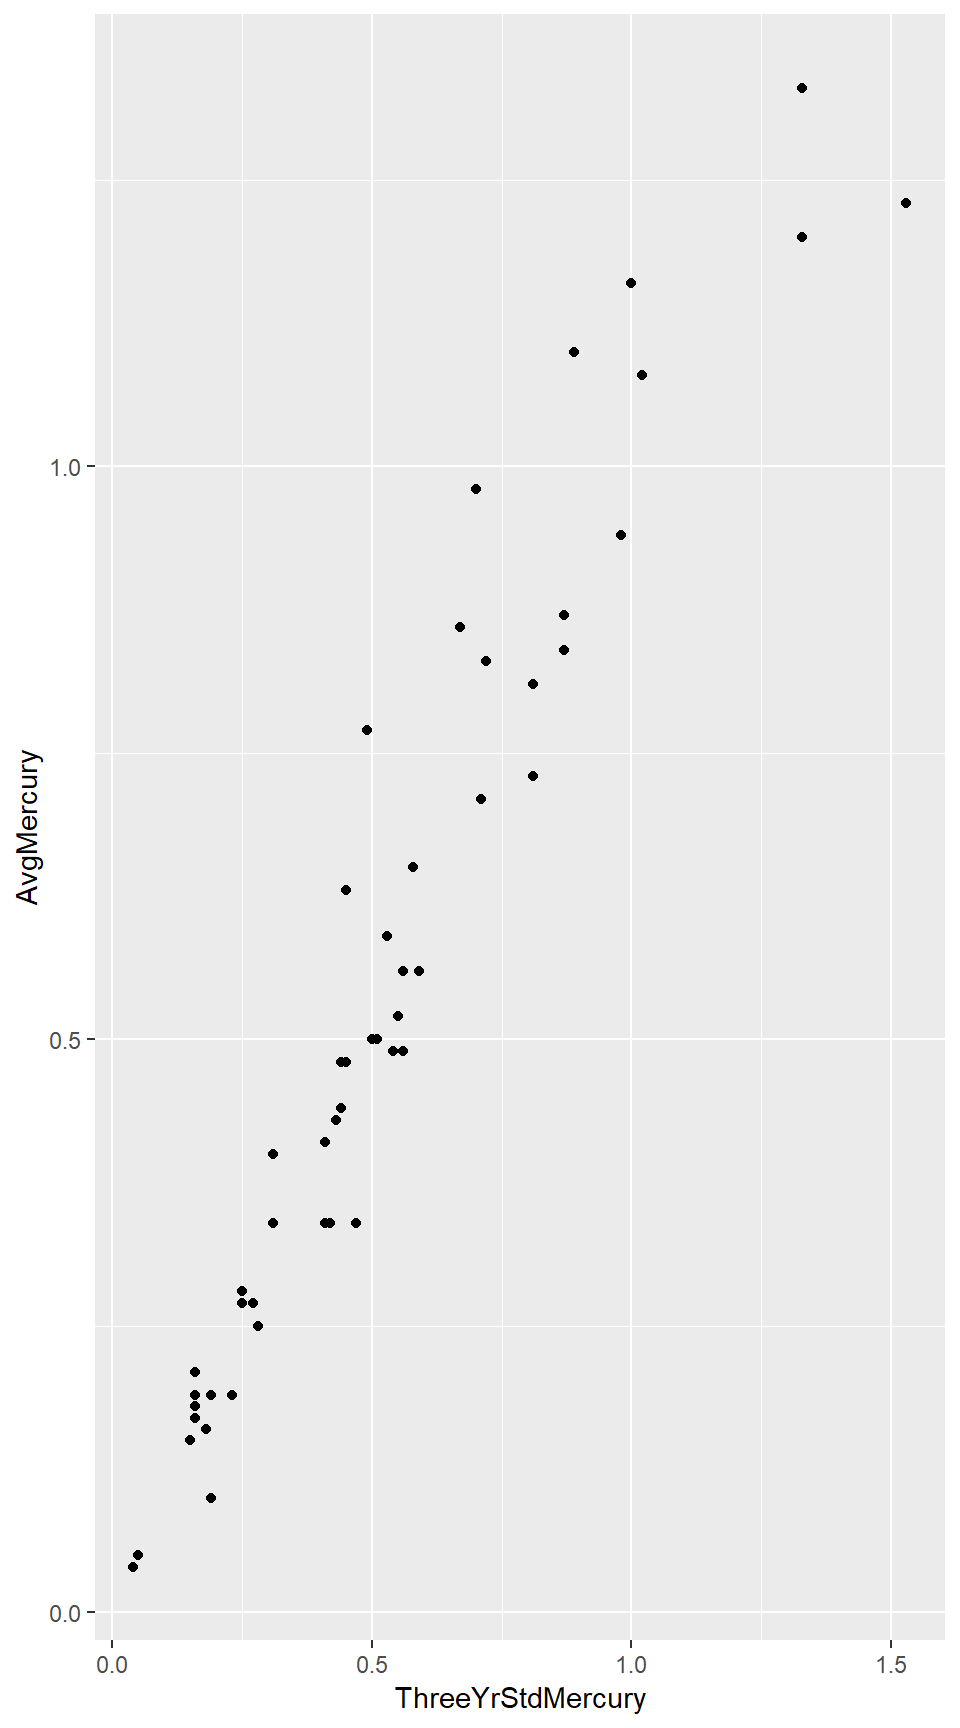
\includegraphics[width=0.65\linewidth]{Lock5WithR_files/figure-latex/Figure2.49-4}

\hypertarget{summarizing-a-relationship-between-two-quantitative-variables-correlation}{%
\subsection{Summarizing a Relationship between Two Quantitative Variables: Correlation}\label{summarizing-a-relationship-between-two-quantitative-variables-correlation}}

Another key numerical statistic is the \textbf{correlation}--the correlation is a measure of the strength and direction of the relationship between two quantitative variables.

\begin{Shaded}
\begin{Highlighting}[]
\KeywordTok{cor}\NormalTok{(Margin }\OperatorTok{~}\StringTok{ }\NormalTok{Approval, }\DataTypeTok{data =}\NormalTok{ ElectionMargin)}
\end{Highlighting}
\end{Shaded}

\begin{verbatim}
## [1] 0.8629926
\end{verbatim}

\begin{Shaded}
\begin{Highlighting}[]
\KeywordTok{cor}\NormalTok{(AvgMercury }\OperatorTok{~}\StringTok{ }\NormalTok{pH, }\DataTypeTok{data =}\NormalTok{ FloridaLakes)}
\end{Highlighting}
\end{Shaded}

\begin{verbatim}
## [1] -0.5754001
\end{verbatim}

\begin{Shaded}
\begin{Highlighting}[]
\KeywordTok{cor}\NormalTok{(AvgMercury }\OperatorTok{~}\StringTok{ }\NormalTok{Alkalinity, }\DataTypeTok{data =}\NormalTok{ FloridaLakes)}
\end{Highlighting}
\end{Shaded}

\begin{verbatim}
## [1] -0.5938967
\end{verbatim}

\begin{Shaded}
\begin{Highlighting}[]
\KeywordTok{cor}\NormalTok{(Alkalinity }\OperatorTok{~}\StringTok{ }\NormalTok{pH, }\DataTypeTok{data =}\NormalTok{ FloridaLakes)}
\end{Highlighting}
\end{Shaded}

\begin{verbatim}
## [1] 0.7191657
\end{verbatim}

\begin{Shaded}
\begin{Highlighting}[]
\KeywordTok{cor}\NormalTok{(AvgMercury }\OperatorTok{~}\StringTok{ }\NormalTok{ThreeYrStdMercury, }\DataTypeTok{data =}\NormalTok{ FloridaLakes)}
\end{Highlighting}
\end{Shaded}

\begin{verbatim}
## [1] 0.9592148
\end{verbatim}

\hypertarget{table-2.31}{%
\subsubsection{Table 2.31}\label{table-2.31}}

\begin{Shaded}
\begin{Highlighting}[]
\NormalTok{CricketChirps}
\end{Highlighting}
\end{Shaded}

\begin{verbatim}
##   Temperature Chirps
## 1        54.5     81
## 2        59.5     97
## 3        63.5    103
## 4        67.5    123
## 5        72.0    150
## 6        78.5    182
## 7        83.0    195
\end{verbatim}

\hypertarget{figure-2.50}{%
\subsubsection{Figure 2.50}\label{figure-2.50}}

\begin{Shaded}
\begin{Highlighting}[]
\KeywordTok{gf_point}\NormalTok{(Temperature }\OperatorTok{~}\StringTok{ }\NormalTok{Chirps, }\DataTypeTok{data =}\NormalTok{ CricketChirps)}
\end{Highlighting}
\end{Shaded}

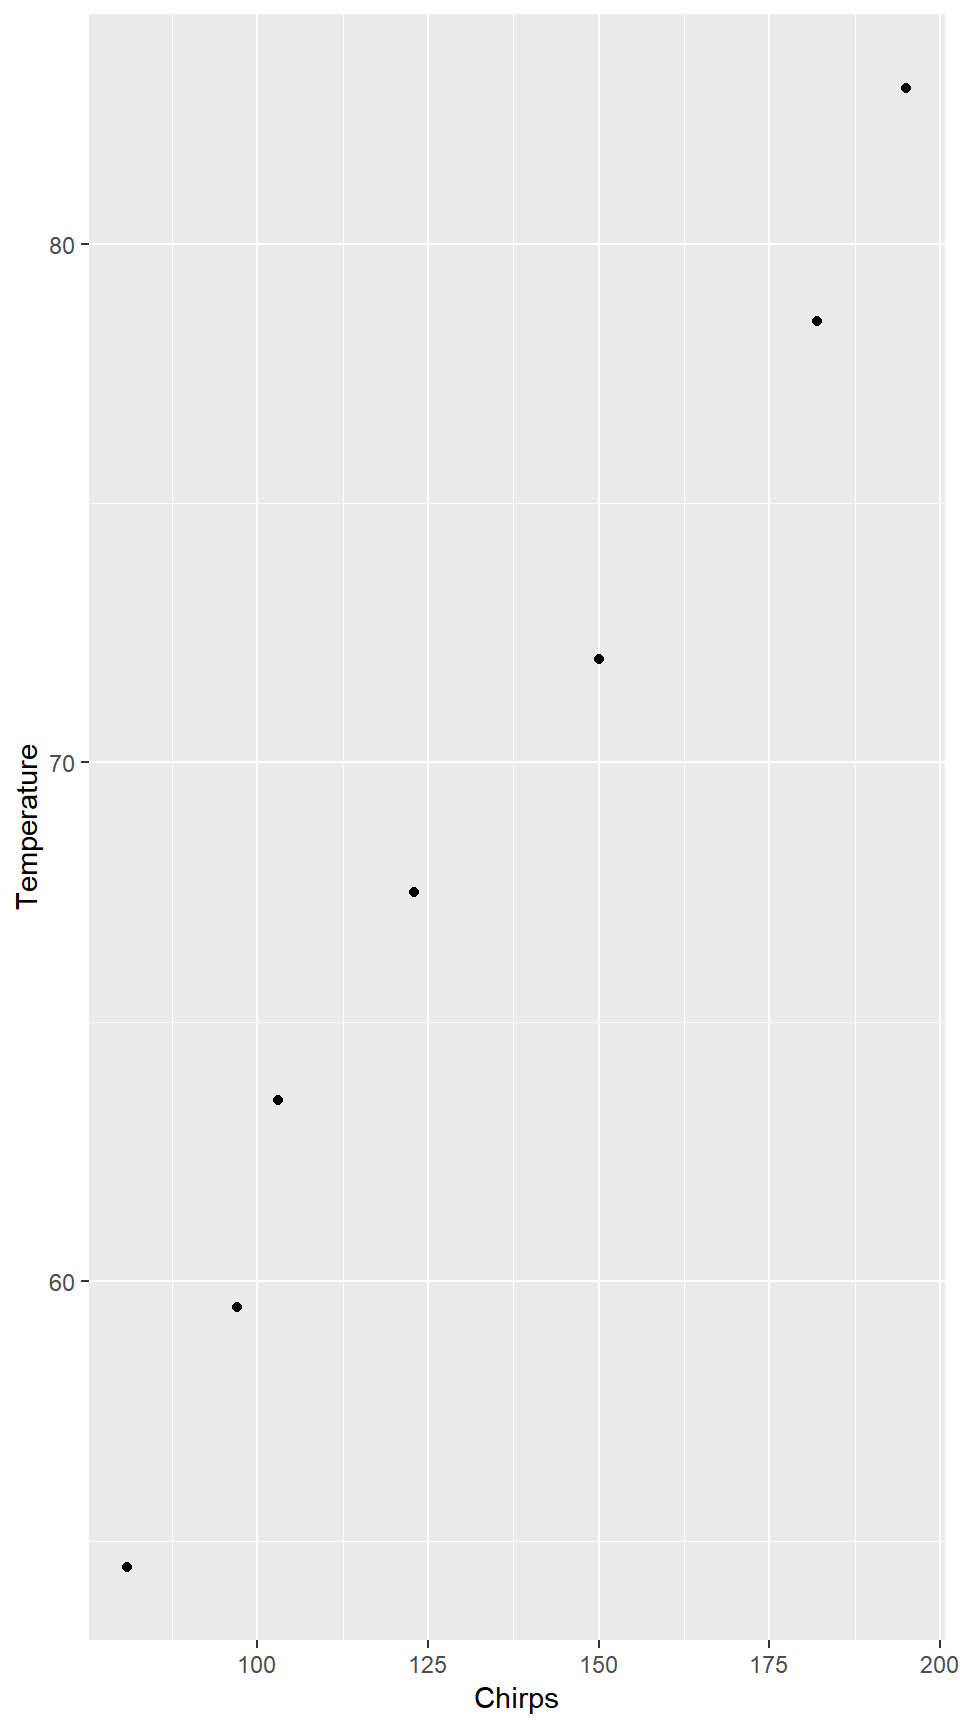
\includegraphics[width=0.65\linewidth]{Lock5WithR_files/figure-latex/Figure2.50-1}

\hypertarget{example-2.35}{%
\subsubsection{Example 2.35}\label{example-2.35}}

\begin{Shaded}
\begin{Highlighting}[]
\KeywordTok{cor}\NormalTok{(Temperature }\OperatorTok{~}\StringTok{ }\NormalTok{Chirps, }\DataTypeTok{data =}\NormalTok{ CricketChirps)}
\end{Highlighting}
\end{Shaded}

\begin{verbatim}
## [1] 0.9906249
\end{verbatim}

\hypertarget{example-2.38}{%
\subsubsection{Example 2.38}\label{example-2.38}}

Further, using the \texttt{subset()()} function again, we can investigate the correlation between variables with some restrictions.

\begin{Shaded}
\begin{Highlighting}[]
\KeywordTok{gf_point}\NormalTok{(Alcohol }\OperatorTok{~}\StringTok{ }\NormalTok{Calories, }\DataTypeTok{data =} \KeywordTok{subset}\NormalTok{(NutritionStudy, Age}\OperatorTok{>}\DecValTok{59}\NormalTok{))}
\end{Highlighting}
\end{Shaded}

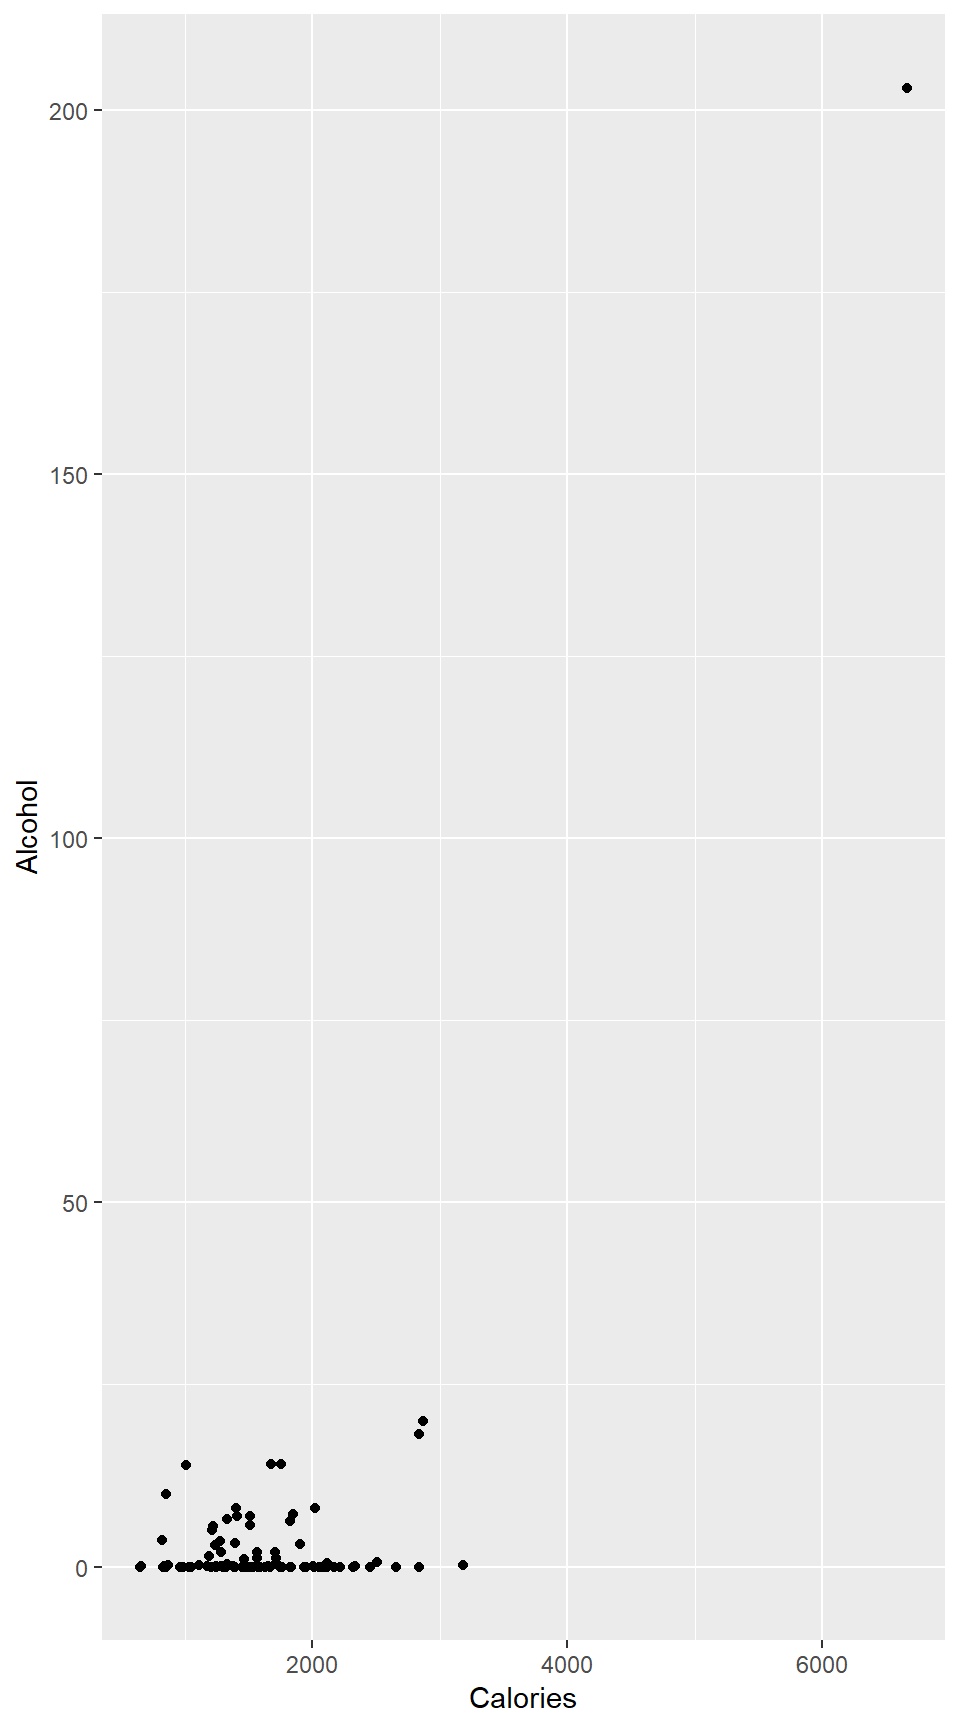
\includegraphics[width=0.65\linewidth]{Lock5WithR_files/figure-latex/Example2.38-1}

\begin{Shaded}
\begin{Highlighting}[]
\KeywordTok{cor}\NormalTok{(Alcohol }\OperatorTok{~}\StringTok{ }\NormalTok{Calories, }\DataTypeTok{data =} \KeywordTok{subset}\NormalTok{(NutritionStudy, Age}\OperatorTok{>}\DecValTok{59}\NormalTok{))}
\end{Highlighting}
\end{Shaded}

\begin{verbatim}
## [1] 0.7199945
\end{verbatim}

And now we omit the outlier

\begin{Shaded}
\begin{Highlighting}[]
\NormalTok{NutritionStudy60 =}\StringTok{ }\KeywordTok{subset}\NormalTok{(NutritionStudy, Age}\OperatorTok{>}\DecValTok{59}\NormalTok{)}
\KeywordTok{gf_point}\NormalTok{(Alcohol }\OperatorTok{~}\StringTok{ }\NormalTok{Calories, }\DataTypeTok{data =} \KeywordTok{subset}\NormalTok{(NutritionStudy60, Alcohol}\OperatorTok{<}\DecValTok{25}\NormalTok{))}
\end{Highlighting}
\end{Shaded}

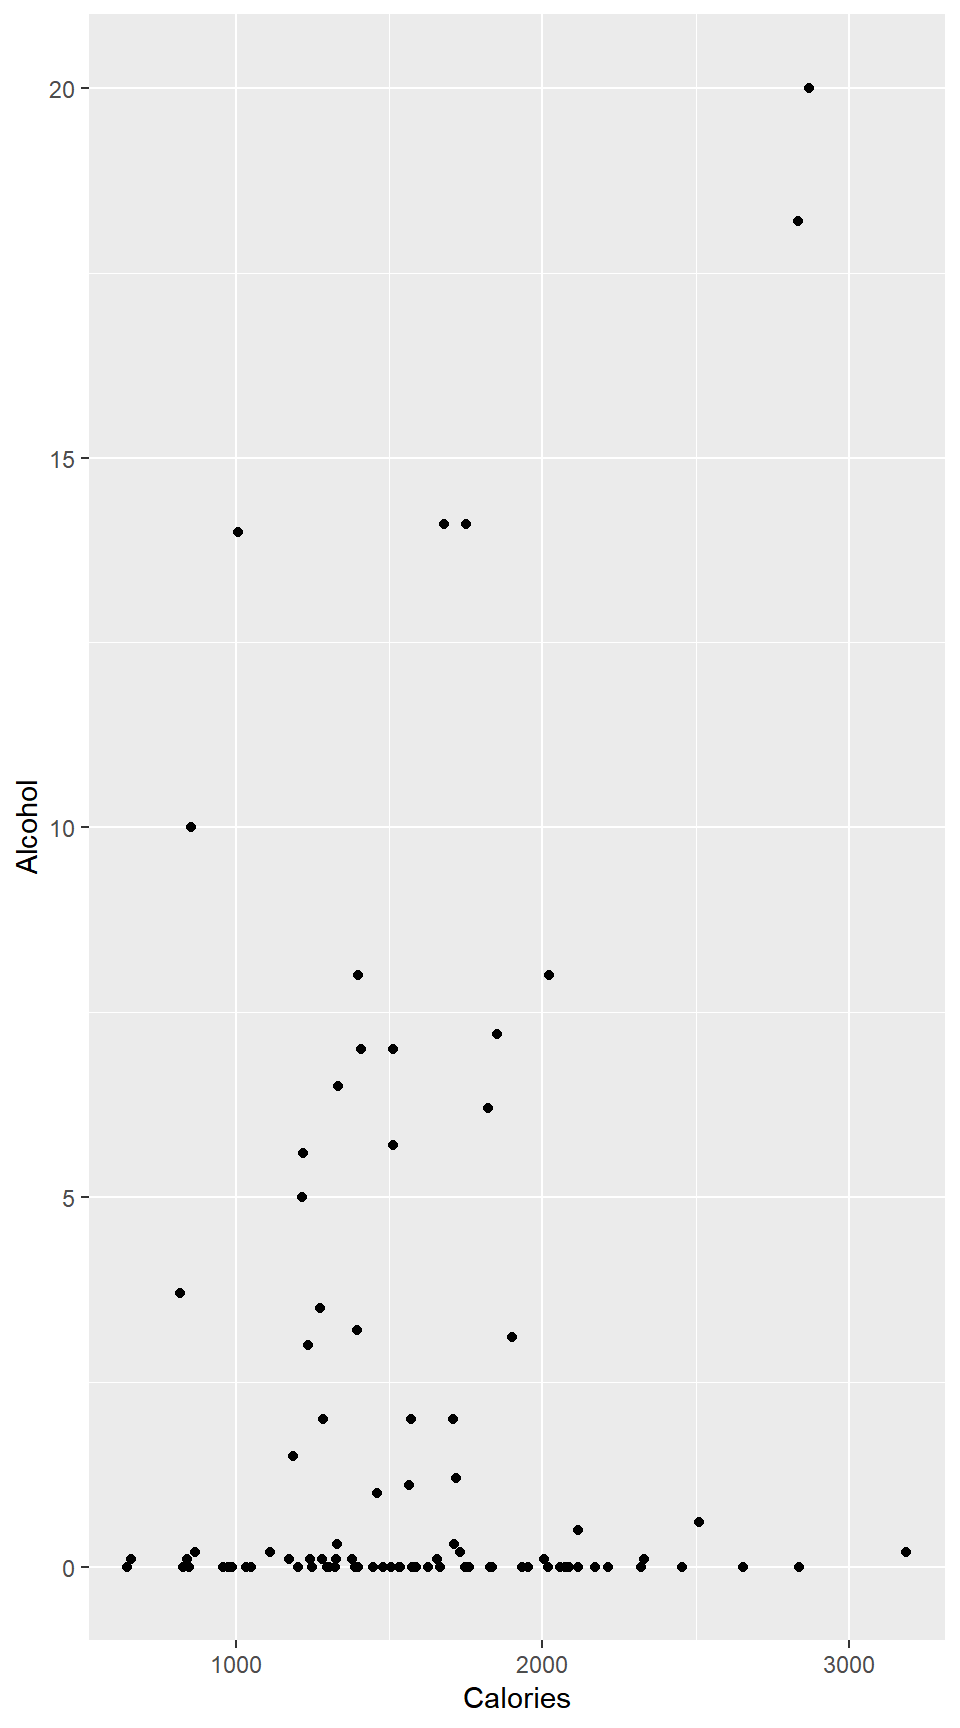
\includegraphics[width=0.65\linewidth]{Lock5WithR_files/figure-latex/Example2.38b-1}

\begin{Shaded}
\begin{Highlighting}[]
\KeywordTok{cor}\NormalTok{(Alcohol }\OperatorTok{~}\StringTok{ }\NormalTok{Calories, }\DataTypeTok{data =} \KeywordTok{subset}\NormalTok{(NutritionStudy60, Alcohol}\OperatorTok{<}\DecValTok{25}\NormalTok{))}
\end{Highlighting}
\end{Shaded}

\begin{verbatim}
## [1] 0.1449633
\end{verbatim}

\hypertarget{two-quantitative-variables-linear-regression}{%
\section{Two Quantitative Variables: Linear Regression}\label{two-quantitative-variables-linear-regression}}

\hypertarget{figure-2.63}{%
\subsubsection{Figure 2.63}\label{figure-2.63}}

\begin{Shaded}
\begin{Highlighting}[]
\KeywordTok{gf_point}\NormalTok{(Tip }\OperatorTok{~}\StringTok{ }\NormalTok{Bill, }\DataTypeTok{size =} \FloatTok{.5}\NormalTok{, }\DataTypeTok{data =}\NormalTok{ RestaurantTips)}
\end{Highlighting}
\end{Shaded}

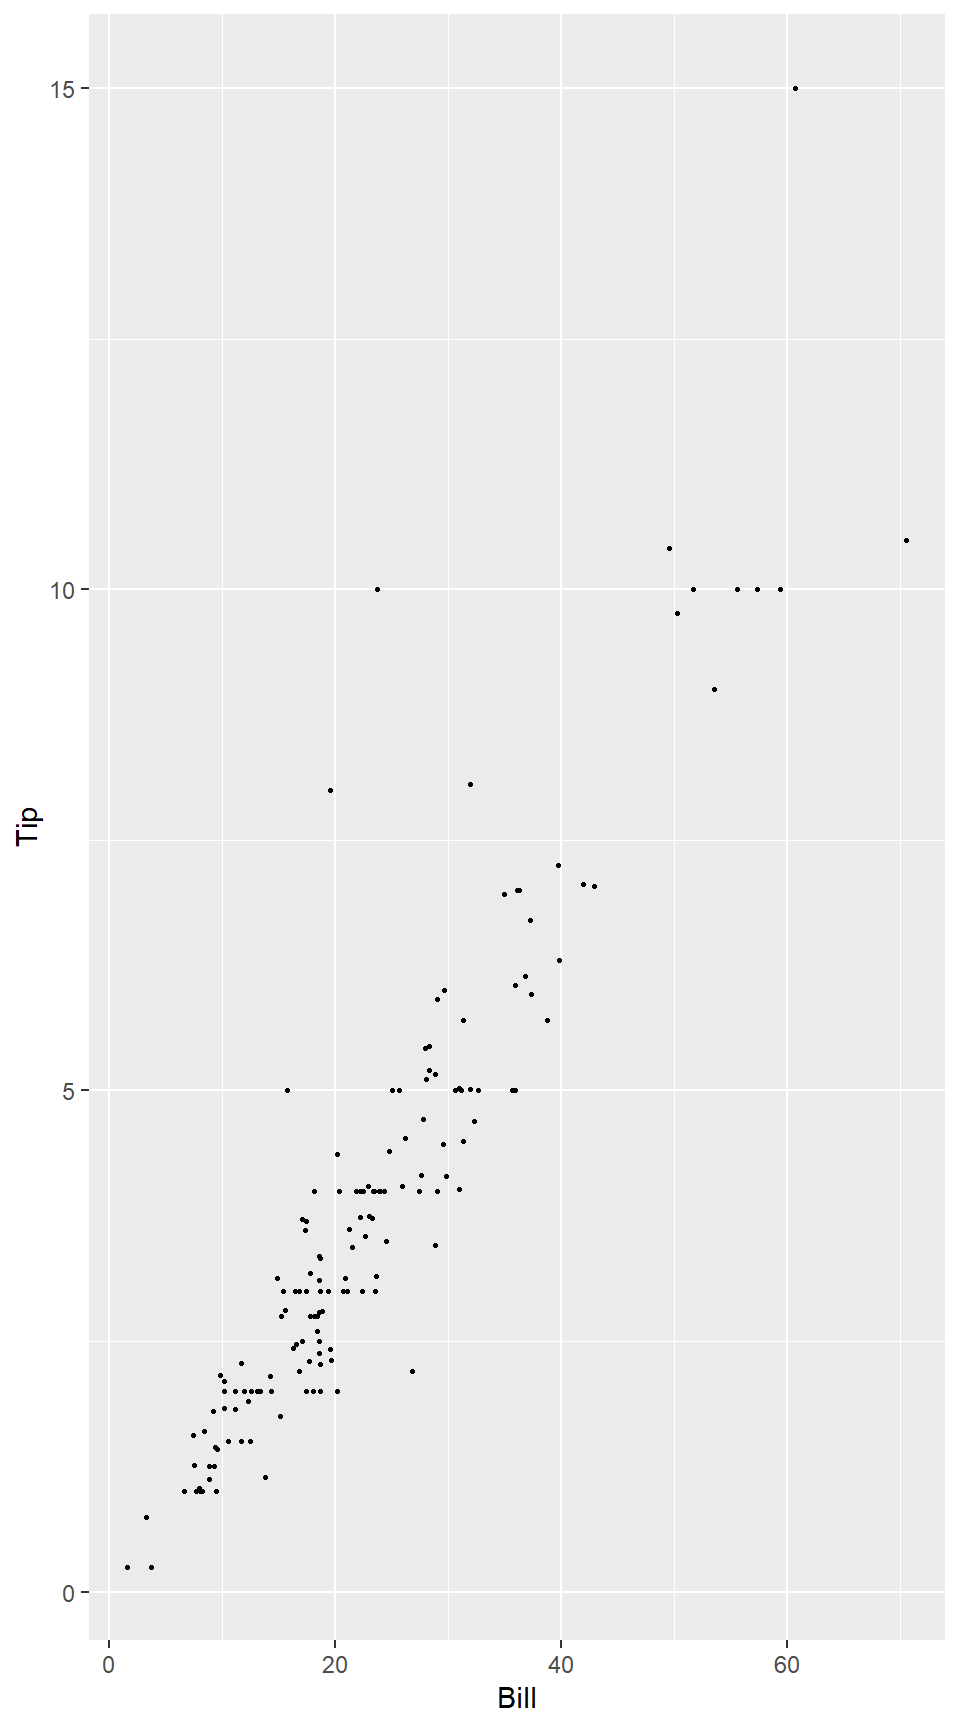
\includegraphics[width=0.65\linewidth]{Lock5WithR_files/figure-latex/Figure2.63-1}

\hypertarget{example-2.39}{%
\subsubsection{Example 2.39}\label{example-2.39}}

When the relationship between variables is sufficiently \emph{linear}, you may be able to predict the value of a variable using the other variable. This is possible by fitting a \emph{regression line}. To plot this in R all we need to do is chain \texttt{gf\_lim()()} to the scatter plot and give it the corresponding arguments.

\begin{Shaded}
\begin{Highlighting}[]
\KeywordTok{gf_point}\NormalTok{(Tip }\OperatorTok{~}\StringTok{ }\NormalTok{Bill, }\DataTypeTok{cex =} \FloatTok{0.5}\NormalTok{, }\DataTypeTok{data =}\NormalTok{ RestaurantTips) }\OperatorTok\StringTok{ }\KeywordTok{gf_lm}\NormalTok{(Tip }\OperatorTok{~}\StringTok{ }\NormalTok{Bill, }\DataTypeTok{data =}\NormalTok{ RestaurantTips)}
\end{Highlighting}
\end{Shaded}

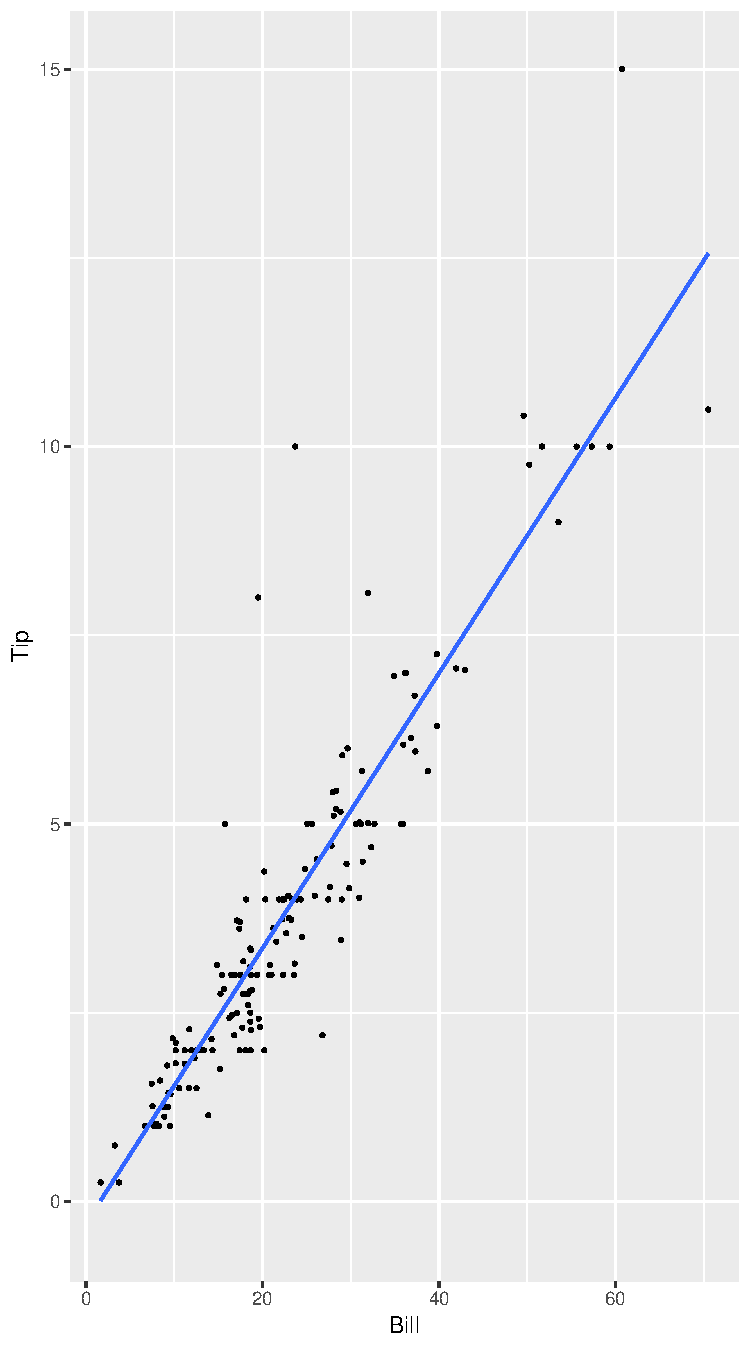
\includegraphics[width=0.65\linewidth]{Lock5WithR_files/figure-latex/Example2.39-1}

\begin{Shaded}
\begin{Highlighting}[]
\KeywordTok{cor}\NormalTok{(Tip }\OperatorTok{~}\StringTok{ }\NormalTok{Bill, }\DataTypeTok{data =}\NormalTok{ RestaurantTips)}
\end{Highlighting}
\end{Shaded}

\begin{verbatim}
## [1] 0.9150592
\end{verbatim}

The equation for the regression line, or the \emph{prediction equation} is
\[
\widehat{\mbox{Response}} = a + b \cdot \mbox{Explanatory}
\]

So now, we need to find the values for a, the intercept, and b, the slope using the function to fit linear models.

\hypertarget{example-2.41}{%
\subsubsection{Example 2.41}\label{example-2.41}}

\begin{Shaded}
\begin{Highlighting}[]
\KeywordTok{lm}\NormalTok{(Tip }\OperatorTok{~}\StringTok{ }\NormalTok{Bill, }\DataTypeTok{data =}\NormalTok{ RestaurantTips)}
\end{Highlighting}
\end{Shaded}

\begin{verbatim}
## 
## Call:
## lm(formula = Tip ~ Bill, data = RestaurantTips)
## 
## Coefficients:
## (Intercept)         Bill  
##     -0.2923       0.1822
\end{verbatim}

\begin{Shaded}
\begin{Highlighting}[]
\KeywordTok{coef}\NormalTok{(}\KeywordTok{lm}\NormalTok{(Tip }\OperatorTok{~}\StringTok{ }\NormalTok{Bill, }\DataTypeTok{data =}\NormalTok{ RestaurantTips))  }\CommentTok{# just show me the coefficients}
\end{Highlighting}
\end{Shaded}

\begin{verbatim}
## (Intercept)        Bill 
##  -0.2922675   0.1822147
\end{verbatim}

This results in the equation
\[
\widehat{\mbox{Tip}} = \Sexpr{tip.coefs$Intercept} + \Sexpr{tip.coefs$Bill} \cdot \mbox{Bill}
\]

With this equation, one can predict the tip for different bill amounts.

\begin{Shaded}
\begin{Highlighting}[]
\NormalTok{Tip.Fun <-}\StringTok{ }\KeywordTok{makeFun}\NormalTok{(}\KeywordTok{lm}\NormalTok{(Tip }\OperatorTok{~}\StringTok{ }\NormalTok{Bill, }\DataTypeTok{data =}\NormalTok{ RestaurantTips)) }\CommentTok{# make a function of the linear model}
\KeywordTok{Tip.Fun}\NormalTok{(}\DataTypeTok{Bill =} \FloatTok{59.33}\NormalTok{) }\CommentTok{# predicted tip when bill is $59.33}
\end{Highlighting}
\end{Shaded}

\begin{verbatim}
##        1 
## 10.51853
\end{verbatim}

\begin{Shaded}
\begin{Highlighting}[]
\KeywordTok{Tip.Fun}\NormalTok{(}\DataTypeTok{Bill =} \FloatTok{9.52}\NormalTok{)}
\end{Highlighting}
\end{Shaded}

\begin{verbatim}
##        1 
## 1.442417
\end{verbatim}

\begin{Shaded}
\begin{Highlighting}[]
\KeywordTok{Tip.Fun}\NormalTok{(}\DataTypeTok{Bill =} \FloatTok{23.70}\NormalTok{)}
\end{Highlighting}
\end{Shaded}

\begin{verbatim}
##        1 
## 4.026222
\end{verbatim}

An important aspect of the linear regression is the difference between the prediction and actual observation. This is called the \textbf{residual}, defined

\[
\mbox{residual} = \mbox{observed response} - \mbox{predicted response}
\]

\hypertarget{example-2.42}{%
\subsubsection{Example 2.42}\label{example-2.42}}

\begin{Shaded}
\begin{Highlighting}[]
\NormalTok{Resid.a <-}\StringTok{ }\FloatTok{10.00} \OperatorTok{-}\StringTok{ }\FloatTok{10.51} \CommentTok{# predicted tip from Example 2.41}
\NormalTok{Resid.a}
\end{Highlighting}
\end{Shaded}

\begin{verbatim}
## [1] -0.51
\end{verbatim}

\begin{Shaded}
\begin{Highlighting}[]
\NormalTok{Resid.b <-}\StringTok{ }\FloatTok{1.00} \OperatorTok{-}\StringTok{ }\FloatTok{1.44}
\NormalTok{Resid.b}
\end{Highlighting}
\end{Shaded}

\begin{verbatim}
## [1] -0.44
\end{verbatim}

\begin{Shaded}
\begin{Highlighting}[]
\NormalTok{Resid.c <-}\StringTok{ }\FloatTok{10.00} \OperatorTok{-}\StringTok{ }\FloatTok{4.02}
\NormalTok{Resid.c}
\end{Highlighting}
\end{Shaded}

\begin{verbatim}
## [1] 5.98
\end{verbatim}

\hypertarget{example-2.43}{%
\subsubsection{Example 2.43}\label{example-2.43}}

\begin{Shaded}
\begin{Highlighting}[]
\NormalTok{Elect.mod <-}\StringTok{ }\KeywordTok{lm}\NormalTok{(Margin}\OperatorTok{~}\NormalTok{Approval, }\DataTypeTok{data =}\NormalTok{ ElectionMargin)}
\KeywordTok{resid}\NormalTok{(}\KeywordTok{lm}\NormalTok{(Margin}\OperatorTok{~}\NormalTok{Approval, }\DataTypeTok{data =}\NormalTok{ ElectionMargin))}
\end{Highlighting}
\end{Shaded}

\begin{verbatim}
##          1          2          3          4          5          6 
## -5.3228564 -0.7958766 -6.6075096  3.0992354 12.0550519 -5.7247133 
##          7          8          9         10         11 
##  0.8801748  7.0550519 -1.6044784 -0.9737848 -2.0602949
\end{verbatim}

\hypertarget{example-2.45}{%
\subsubsection{Example 2.45}\label{example-2.45}}

\begin{Shaded}
\begin{Highlighting}[]
\KeywordTok{lm}\NormalTok{(AvgMercury }\OperatorTok{~}\StringTok{ }\NormalTok{pH, }\DataTypeTok{data =}\NormalTok{ FloridaLakes)}
\end{Highlighting}
\end{Shaded}

\begin{verbatim}
## 
## Call:
## lm(formula = AvgMercury ~ pH, data = FloridaLakes)
## 
## Coefficients:
## (Intercept)           pH  
##      1.5309      -0.1523
\end{verbatim}

\begin{Shaded}
\begin{Highlighting}[]
\KeywordTok{gf_point}\NormalTok{(AvgMercury }\OperatorTok{~}\StringTok{ }\NormalTok{pH, }\DataTypeTok{data =}\NormalTok{ FloridaLakes) }\OperatorTok\StringTok{ }\KeywordTok{gf_lm}\NormalTok{(AvgMercury }\OperatorTok{~}\StringTok{ }\NormalTok{pH, }\DataTypeTok{data =}\NormalTok{ FloridaLakes)}
\end{Highlighting}
\end{Shaded}

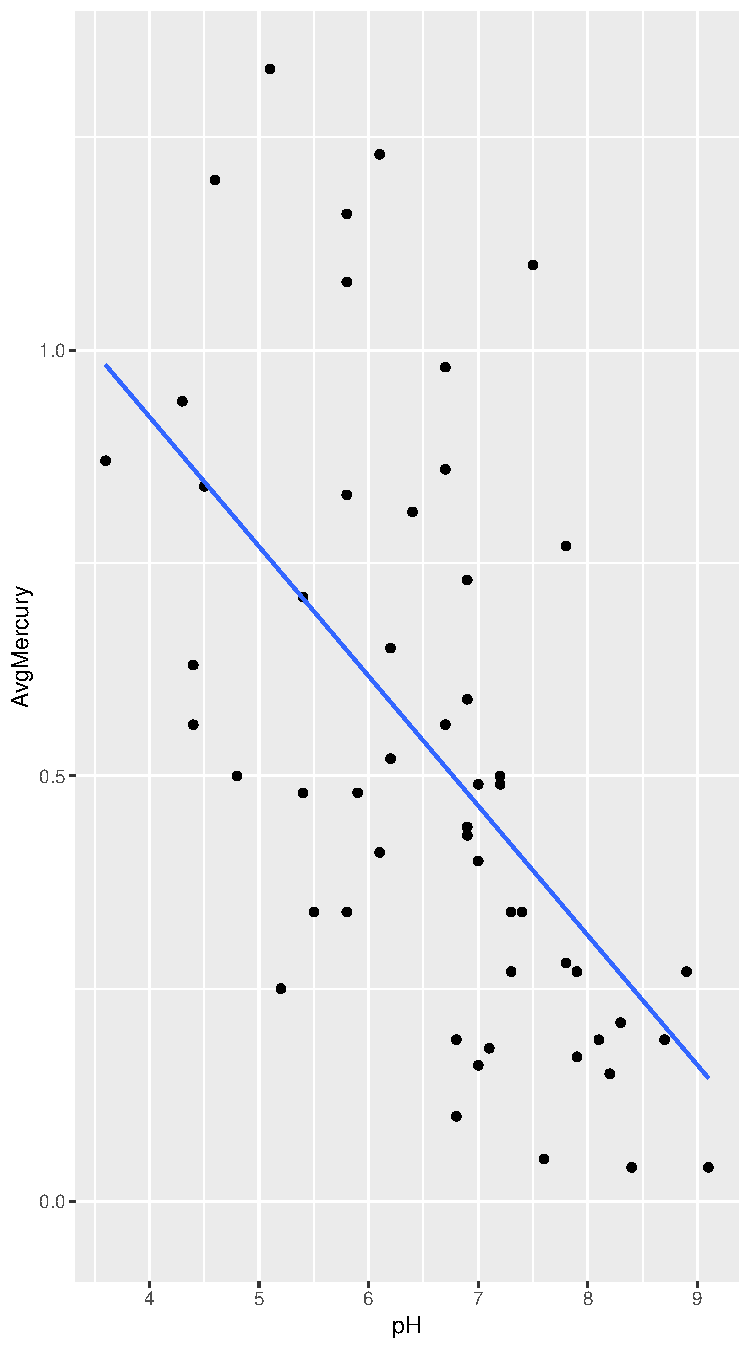
\includegraphics[width=0.65\linewidth]{Lock5WithR_files/figure-latex/Example2.45-1}

\begin{Shaded}
\begin{Highlighting}[]
\NormalTok{Mer.Fun <-}\StringTok{ }\KeywordTok{makeFun}\NormalTok{(}\KeywordTok{lm}\NormalTok{(AvgMercury }\OperatorTok{~}\StringTok{ }\NormalTok{pH, }\DataTypeTok{data =}\NormalTok{ FloridaLakes))}
\KeywordTok{Mer.Fun}\NormalTok{(}\DataTypeTok{pH =} \FloatTok{7.5}\NormalTok{) }\CommentTok{# predicted mercury level at 7.5 pH}
\end{Highlighting}
\end{Shaded}

\begin{verbatim}
##         1 
## 0.3886622
\end{verbatim}

\begin{Shaded}
\begin{Highlighting}[]
\NormalTok{Resid <-}\StringTok{ }\FloatTok{1.10} \OperatorTok{-}\StringTok{ }\FloatTok{0.388} \CommentTok{# residual at 7.5 pH}
\NormalTok{Resid}
\end{Highlighting}
\end{Shaded}

\begin{verbatim}
## [1] 0.712
\end{verbatim}

\hypertarget{example-2.46}{%
\subsubsection{Example 2.46}\label{example-2.46}}

\begin{Shaded}
\begin{Highlighting}[]
\NormalTok{Cal.Fun <-}\StringTok{ }\KeywordTok{makeFun}\NormalTok{(}\KeywordTok{lm}\NormalTok{(Calcium }\OperatorTok{~}\StringTok{ }\NormalTok{pH, }\DataTypeTok{data =}\NormalTok{ FloridaLakes))}
\NormalTok{Cal.Fun}
\end{Highlighting}
\end{Shaded}

\begin{verbatim}
## function (pH, ..., transformation = function (x) 
## x) 
## return(transformation(predict(model, newdata = data.frame(pH = pH), 
##     ...)))
## <environment: 0x000000001dd7c2e0>
## attr(,"coefficients")
## (Intercept)          pH 
##   -51.40157    11.16800
\end{verbatim}

\hypertarget{figure-2.68}{%
\subsubsection{Figure 2.68}\label{figure-2.68}}

\begin{Shaded}
\begin{Highlighting}[]
\KeywordTok{gf_point}\NormalTok{(Calcium }\OperatorTok{~}\StringTok{ }\NormalTok{pH, }\DataTypeTok{data =}\NormalTok{ FloridaLakes) }\OperatorTok\StringTok{ }\KeywordTok{gf_lm}\NormalTok{(Calcium }\OperatorTok{~}\StringTok{ }\NormalTok{pH, }\DataTypeTok{data =}\NormalTok{ FloridaLakes)}
\end{Highlighting}
\end{Shaded}

\includegraphics[width=0.65\linewidth]{Lock5WithR_files/figure-latex/Figure2.68-1}

\hypertarget{graphical-summaries-important-ideas}{%
\section{Graphical Summaries -- Important Ideas}\label{graphical-summaries-important-ideas}}

\hypertarget{patterns-and-deviations-from-patterns}{%
\subsection{Patterns and Deviations from Patterns}\label{patterns-and-deviations-from-patterns}}

The goal of a statistical plot is to help us see

\begin{enumerate}
\tightlist
\item
  potential patterns in the data, and
\item
  deviations from those patterns.\\
\end{enumerate}

\hypertarget{different-plots-for-different-kinds-of-variables}{%
\subsection{Different Plots for Different Kinds of Variables}\label{different-plots-for-different-kinds-of-variables}}

Graphical summaries can help us see the \emph{distribution} of a variable
or the \emph{relationships} between two (or more) variables. The type of plot
used will depend on the kinds of variables involved. You can use \texttt{demo()()} to see how
to get R to make the plots in this section.

When we do statistical analysis, we will see that the analysis we use will
also depend on the kinds of variables involved, so this is an important idea.

\hypertarget{side-by-side-plots-and-overlays-can-reveal-importance-of-additional-factors}{%
\subsection{Side-by-side Plots and Overlays Can Reveal Importance of Additional Factors}\label{side-by-side-plots-and-overlays-can-reveal-importance-of-additional-factors}}

The \textbf{\texttt{ggformula}} graphics plots make it particularly easy to generate plots that
divide the data into groups and either produce a panel for each group (using \textbar!)
or display each group in a different way (different colors or symbols, using
the {fill} or {colour} arguments). These plots can reveal the
possible influence of additional variables -- sometimes called covariates.

\hypertarget{area-relative-frequency}{%
\subsection{Area = (relative) frequency}\label{area-relative-frequency}}

Many plots are based on the key idea that our eyes are good at comparing areas. Plots
that use area (e.g., histograms, mosaic plots, bar charts, pie charts) should always obey
this principle

{\%s}Area \(=\) (relative) frequency
Plots that violate this principle can be deceptive and distort the true nature
of the data.

\hypertarget{an-example-histogram-with-unequal-bin-widths}{%
\subsection{An Example: Histogram with unequal bin widths}\label{an-example-histogram-with-unequal-bin-widths}}

It is possible to make histograms with bins that have different widths.
But in this case it is important that the height of the bars is chosen so
that area (\emph{NOT height}) is proportional to frequency.\\
Using height instead of area would distort the picture.

When unequal bin sizes are specified, you should use \texttt{gf\_dhistogram()()}

\begin{Shaded}
\begin{Highlighting}[]
\KeywordTok{gf_dhistogram}\NormalTok{( }\OperatorTok{~}\StringTok{ }\NormalTok{Sepal.Length, }\DataTypeTok{data =}\NormalTok{ iris, }\DataTypeTok{breaks =} \KeywordTok{c}\NormalTok{(}\DecValTok{4}\NormalTok{,}\DecValTok{5}\NormalTok{,}\FloatTok{5.5}\NormalTok{,}\FloatTok{5.75}\NormalTok{,}\DecValTok{6}\NormalTok{,}\FloatTok{6.5}\NormalTok{,}\DecValTok{7}\NormalTok{,}\DecValTok{8}\NormalTok{,}\DecValTok{9}\NormalTok{))}
\end{Highlighting}
\end{Shaded}

\includegraphics[width=0.65\linewidth]{Lock5WithR_files/figure-latex/hist-unequal-bins-1}

The density scale is important.
It tells R to use a scale such that
the area (height \$Ã--- width) of the rectangles is equal to the relative frequency.
For example, the bar from 5.0 to 5.5 has width \(\frac12\) and height about \(0.36\), so
the area is \(0.18\), which means approximately 18\% of the sepal lengths are
between 5.0 and 5.5.

It would be incorrect to choose \texttt{gf\_histogram()()} since
this distorts the picture of the data.

\begin{Shaded}
\begin{Highlighting}[]
\KeywordTok{gf_histogram}\NormalTok{( }\OperatorTok{~}\StringTok{ }\NormalTok{Sepal.Length, }\DataTypeTok{data =}\NormalTok{ iris, }\DataTypeTok{breaks =} \KeywordTok{c}\NormalTok{(}\DecValTok{4}\NormalTok{,}\DecValTok{5}\NormalTok{,}\FloatTok{5.5}\NormalTok{,}\FloatTok{5.75}\NormalTok{,}\DecValTok{6}\NormalTok{,}\FloatTok{6.5}\NormalTok{,}\DecValTok{7}\NormalTok{,}\DecValTok{8}\NormalTok{,}\DecValTok{9}\NormalTok{))}
\end{Highlighting}
\end{Shaded}

Notice how different this looks. Now the heights are equal to the relative
frequency, but this makes the wider bars have too much area.

\hypertarget{more-on-plots}{%
\section{More on Plots}\label{more-on-plots}}

There are lots of arguments that control how these plots look. Here are just a
few examples, some of which we have already seen.

\hypertarget{show.legend}{%
\subsection{show.legend}\label{show.legend}}

{show.legend = TRUE} turns on a simple legend for the grouping variable.\\
(There are ways to have more control, if you need it.) It is on by default in ggformula plots

\begin{Shaded}
\begin{Highlighting}[]
\KeywordTok{gf_point}\NormalTok{(Sepal.Length }\OperatorTok{~}\StringTok{ }\NormalTok{Sepal.Width, }\DataTypeTok{colour =} \OperatorTok{~}\NormalTok{Species, }\DataTypeTok{data =}\NormalTok{ iris, }
    \DataTypeTok{show.legend =} \OtherTok{TRUE}\NormalTok{)}
\end{Highlighting}
\end{Shaded}

\includegraphics[width=0.65\linewidth]{Lock5WithR_files/figure-latex/iris-xyplot-key-1}

\hypertarget{alpha-cex}{%
\subsection{alpha, cex}\label{alpha-cex}}

Sometimes it is nice to have elements of a plot be partly transparent. When
such elements overlap, they get darker, showing us where data are ``piling up.''
Setting the {alpha} argument to a value between 0 and 1 controls the
degree of transparency: 1 is completely opaque, 0 is invisible. The
{dotsize} for \texttt{gf\_dotplot()()} and {size} for \texttt{gf\_point()()} arguments control ``character expansion'' and can be used to make
the plotting ``characters'' larger or smaller by specifying the scaling ratio.

Here is another example using data on 150 iris plants of three species.

\begin{Shaded}
\begin{Highlighting}[]
\KeywordTok{xyplot}\NormalTok{(Sepal.Length }\OperatorTok{~}\StringTok{ }\NormalTok{Sepal.Width, }\DataTypeTok{groups =}\NormalTok{ Species, }\DataTypeTok{data =}\NormalTok{ iris, }
    \DataTypeTok{auto.key =} \KeywordTok{list}\NormalTok{(}\DataTypeTok{columns =} \DecValTok{3}\NormalTok{),}
    \DataTypeTok{alpha =} \FloatTok{.5}\NormalTok{,}
    \DataTypeTok{cex =} \FloatTok{1.3}\NormalTok{)   }
\end{Highlighting}
\end{Shaded}

\includegraphics[width=0.65\linewidth]{Lock5WithR_files/figure-latex/iris-xyplot-alpha-1}

\begin{Shaded}
\begin{Highlighting}[]
\KeywordTok{gf_point}\NormalTok{(Sepal.Length }\OperatorTok{~}\StringTok{ }\NormalTok{Sepal.Width, }\DataTypeTok{colour =} \OperatorTok{~}\NormalTok{Species, }\DataTypeTok{data =}\NormalTok{ iris, }
    \DataTypeTok{show.legend =} \OtherTok{TRUE}\NormalTok{,}
    \DataTypeTok{alpha =} \FloatTok{.5}\NormalTok{,}
    \DataTypeTok{size =} \FloatTok{1.3}\NormalTok{)  }
\end{Highlighting}
\end{Shaded}

\includegraphics[width=0.65\linewidth]{Lock5WithR_files/figure-latex/iris-xyplot-alpha-2}

\hypertarget{gf_labs-xlab-ylab-title-subtitle}{%
\subsection{gf\_labs(), xlab, ylab, title, subtitle}\label{gf_labs-xlab-ylab-title-subtitle}}

You can add a title or subtitle, or change the default labels of the axes in one of two ways. \texttt{gf\_labs()()} allows the chaining syntax to be used.

\begin{Shaded}
\begin{Highlighting}[]
\KeywordTok{gf_point}\NormalTok{(Sepal.Length }\OperatorTok{~}\StringTok{ }\NormalTok{Sepal.Width, }\DataTypeTok{colour =} \OperatorTok{~}\NormalTok{Species, }\DataTypeTok{data =}\NormalTok{ iris, }\DataTypeTok{alpha =} \FloatTok{.5}\NormalTok{)  }\OperatorTok\StringTok{ }\KeywordTok{gf_labs}\NormalTok{(}
  \DataTypeTok{x =} \StringTok{"sepal width (cm)"}\NormalTok{, }
  \DataTypeTok{y =} \StringTok{"sepal length (cm)"}\NormalTok{, }
  \DataTypeTok{subtitle =} \StringTok{"(R. A. Fisher analysized this data in 1936)"}\NormalTok{, }
  \DataTypeTok{title =} \StringTok{"Some Iris Data"}\NormalTok{)}
\end{Highlighting}
\end{Shaded}

\includegraphics[width=0.65\linewidth]{Lock5WithR_files/figure-latex/iris-xyplot-text-1}

\begin{Shaded}
\begin{Highlighting}[]
\KeywordTok{gf_point}\NormalTok{(Sepal.Length }\OperatorTok{~}\StringTok{ }\NormalTok{Sepal.Width, }\DataTypeTok{colour =} \OperatorTok{~}\NormalTok{Species, }\DataTypeTok{data =}\NormalTok{ iris, }\DataTypeTok{alpha =} \FloatTok{.5}\NormalTok{, }
         \DataTypeTok{xlab =} \StringTok{"sepal width (cm)"}\NormalTok{, }
         \DataTypeTok{ylab =} \StringTok{"sepal length (cm)"}\NormalTok{, }
         \DataTypeTok{subtitle =} \StringTok{"(R. A. Fisher analysized this data in 1936)"}\NormalTok{, }
         \DataTypeTok{title =} \StringTok{"Some Iris Data"}\NormalTok{)}
\end{Highlighting}
\end{Shaded}

\includegraphics[width=0.65\linewidth]{Lock5WithR_files/figure-latex/iris-xyplot-text-2}

\hypertarget{layout}{%
\subsection{layout}\label{layout}}

{layout} can be used to control the arrangement of panels in a multi-panel
plot. The format is

\begin{Shaded}
\begin{Highlighting}[]
\NormalTok{layout =}\StringTok{ }\KeywordTok{c}\NormalTok{(cols, rows)}
\end{Highlighting}
\end{Shaded}

where \texttt{cols} is the number of columns and \texttt{rows} is the number of
rows. (Columns first because that is the \(x\)-coordinate of the plot.)

\hypertarget{size-theme-color-shape}{%
\subsubsection{size, theme, color, shape}\label{size-theme-color-shape}}

These can be used to change the size of the data visual, set theme of the plot, change the color of the data visual and its shape.

\begin{Shaded}
\begin{Highlighting}[]
\KeywordTok{gf_dens}\NormalTok{( }\OperatorTok{~}\NormalTok{age, }\DataTypeTok{data =}\NormalTok{ HELPrct, }\DataTypeTok{colour =} \OperatorTok{~}\NormalTok{sex, }\DataTypeTok{size =} \DecValTok{2}\NormalTok{) }\OperatorTok\StringTok{ }\KeywordTok{gf_theme}\NormalTok{(}\DataTypeTok{theme =} \KeywordTok{theme_dark}\NormalTok{())}
\end{Highlighting}
\end{Shaded}

\includegraphics[width=0.65\linewidth]{Lock5WithR_files/figure-latex/pch-lwd-lty-1}

\begin{Shaded}
\begin{Highlighting}[]
\KeywordTok{gf_histogram}\NormalTok{( }\OperatorTok{~}\StringTok{ }\NormalTok{age, }\DataTypeTok{data =}\NormalTok{ HELPrct, }\DataTypeTok{fill =} \StringTok{'skyblue'}\NormalTok{)}
\end{Highlighting}
\end{Shaded}

\includegraphics[width=0.65\linewidth]{Lock5WithR_files/figure-latex/pch-lwd-lty-2}

\begin{Shaded}
\begin{Highlighting}[]
\CommentTok{# There are 25 numbered plot symbols; shape = plot character}
\KeywordTok{gf_point}\NormalTok{( mcs }\OperatorTok{~}\StringTok{ }\NormalTok{age, }\DataTypeTok{data =}\NormalTok{ HELPrct, }\DataTypeTok{colour =} \OperatorTok{~}\NormalTok{sex, }
        \DataTypeTok{shape =} \DecValTok{8}\NormalTok{, }\DataTypeTok{size =} \DecValTok{2}\NormalTok{ )  }
\end{Highlighting}
\end{Shaded}

\includegraphics[width=0.65\linewidth]{Lock5WithR_files/figure-latex/col-1}

You can a list of the hundreds of available color names using
colors()

\begin{Shaded}
\begin{Highlighting}[]
\KeywordTok{colors}\NormalTok{()}
\end{Highlighting}
\end{Shaded}

\hypertarget{trellis.par.set}{%
\subsection{trellis.par.set()}\label{trellis.par.set}}

Default settings for lattice graphics are set using
\texttt{trellis.par.set()()}.
Don't like the default font sizes? You can change to a 7 point (base) font using

\begin{Shaded}
\begin{Highlighting}[]
\KeywordTok{trellis.par.set}\NormalTok{(}\DataTypeTok{fontsize =} \KeywordTok{list}\NormalTok{(}\DataTypeTok{text =} \DecValTok{7}\NormalTok{))    }\CommentTok{# base size for text is 7 point }
\end{Highlighting}
\end{Shaded}

Nearly every feature of a lattice plot can be controlled: fonts, colors,
symbols, line thicknesses, colors, etc. Rather than describe them all here,
we'll mention only that groups of these settings
can be collected into a theme.\\
\texttt{show.settings()()} will show you what the theme looks like.

\begin{Shaded}
\begin{Highlighting}[]
\KeywordTok{trellis.par.set}\NormalTok{(}\DataTypeTok{theme =} \KeywordTok{col.whitebg}\NormalTok{())      }\CommentTok{# a theme in the lattice package}
\KeywordTok{show.settings}\NormalTok{()}
\end{Highlighting}
\end{Shaded}

\includegraphics[width=0.65\linewidth]{Lock5WithR_files/figure-latex/themes-whitbg-1}

\newpage

\textless\textless themes-mosaic, cache = TRUE, fig.height = 4.0, fig.width = 6, out.height = `.4\textbackslash textheight'\textgreater\textgreater=
trellis.par.set(theme = col.mosaic()) \# a theme in the mosaic package
show.settings()
@
\textless\textless themes-mosaic2, cache = TRUE, fig.height = 4, fig.width = 6, out.height = `.4\textbackslash textheight'\textgreater\textgreater=
trellis.par.set(theme = col.mosaic(bw = TRUE)) \# black and white version
show.settings()
@

\begin{Shaded}
\begin{Highlighting}[]
\KeywordTok{trellis.par.set}\NormalTok{(}\DataTypeTok{theme =} \KeywordTok{col.mosaic}\NormalTok{())       }\CommentTok{# back to the mosaic theme}
\KeywordTok{trellis.par.set}\NormalTok{(}\DataTypeTok{fontsize =} \KeywordTok{list}\NormalTok{(}\DataTypeTok{text =} \DecValTok{9}\NormalTok{))    }\CommentTok{# and back to a 9 point font}
\end{Highlighting}
\end{Shaded}

Want to save your settings?

\begin{Shaded}
\begin{Highlighting}[]
\CommentTok{# save current settings}
\NormalTok{mySettings <-}\StringTok{ }\KeywordTok{trellis.par.get}\NormalTok{()}
\CommentTok{# switch to mosaic defaults}
\KeywordTok{trellis.par.set}\NormalTok{(}\DataTypeTok{theme =} \KeywordTok{col.mosaic}\NormalTok{())}
\CommentTok{# switch back to my saved settings}
\KeywordTok{trellis.par.set}\NormalTok{(mySettings)}
\end{Highlighting}
\end{Shaded}

\hypertarget{exporting-plots}{%
\section{Exporting Plots}\label{exporting-plots}}

You can save plots to files or copy them to the clipboard using the
{ Export } menu in the { Plots } tab. It is quite simple to copy the
plots to the clipboard and then paste them into a Word document, for example.
You can even adjust the height and width of the plot first to get it the
shape you want.

R code and output can be copied and pasted as well. It's best to use a
fixed width font (like Courier) for R code so that things align properly.

RStudio also provides a way (actually multiple ways) to create documents
that include text, R code, R output, and graphics all in one document so you don't
have to do any copying and pasting. This is a much better workflow since it avoids
copy-and-paste which is error prone and makes it easy to regenerate an entire report
should the data change (because you get more of it or correct an error, for example).

\newpage

\hypertarget{exercises}{%
\section{Exercises}\label{exercises}}

For problems 1--\ref{prob:CPSmulti},
include both the plots and the code you used to make them as well as any
required discussion. Once you get the plots figured out, feel free to
use some of the bells and whistles to make the plots even better.

Use R s help system to find out what the {i1} and {i2}
variables are in the {HELPrct} data frame. Make histograms
for each variable and comment on what you find out. How would you describe
the shape of these distributions? Do you see any outliers (observations
that don't seem to fit the pattern of the rest of the data)?\\

Compare the distributions of {i1} and {i2} among men
and women.

\begin{Shaded}
\begin{Highlighting}[]
\KeywordTok{gf_dens}\NormalTok{( }\OperatorTok{~}\NormalTok{i1, }\DataTypeTok{colour =} \OperatorTok{~}\NormalTok{sex, }\DataTypeTok{data =}\NormalTok{ HELPrct )}
\end{Highlighting}
\end{Shaded}

\includegraphics[width=0.65\linewidth]{Lock5WithR_files/figure-latex/unnamed-chunk-21-1}

\begin{Shaded}
\begin{Highlighting}[]
\KeywordTok{gf_dens}\NormalTok{( }\OperatorTok{~}\NormalTok{i2, }\DataTypeTok{colour =} \OperatorTok{~}\NormalTok{sex, }\DataTypeTok{data =}\NormalTok{ HELPrct )}
\end{Highlighting}
\end{Shaded}

\includegraphics[width=0.65\linewidth]{Lock5WithR_files/figure-latex/unnamed-chunk-21-2}

\begin{verbatim}
Compare the distributions of <span style="color:green">i1</span> and <span style="color:green">i2</span> among 
the three <span style="color:green">substance</span> groups.
\end{verbatim}

\begin{Shaded}
\begin{Highlighting}[]
\KeywordTok{gf_dens}\NormalTok{( }\OperatorTok{~}\NormalTok{i1, }\DataTypeTok{colour =} \OperatorTok{~}\NormalTok{substance, }\DataTypeTok{data =}\NormalTok{ HELPrct )}
\end{Highlighting}
\end{Shaded}

\includegraphics[width=0.65\linewidth]{Lock5WithR_files/figure-latex/unnamed-chunk-22-1}

\begin{Shaded}
\begin{Highlighting}[]
\KeywordTok{gf_dens}\NormalTok{( }\OperatorTok{~}\NormalTok{i2, }\DataTypeTok{colour =} \OperatorTok{~}\NormalTok{substance, }\DataTypeTok{data =}\NormalTok{ HELPrct )}
\end{Highlighting}
\end{Shaded}

\includegraphics[width=0.65\linewidth]{Lock5WithR_files/figure-latex/unnamed-chunk-22-2}

\begin{Shaded}
\begin{Highlighting}[]
\KeywordTok{gf_dens}\NormalTok{( }\OperatorTok{~}\NormalTok{i1}\OperatorTok{|}\NormalTok{sex, }\DataTypeTok{colour =} \OperatorTok{~}\NormalTok{substance, }\DataTypeTok{data =}\NormalTok{ HELPrct )}
\end{Highlighting}
\end{Shaded}

\includegraphics[width=0.65\linewidth]{Lock5WithR_files/figure-latex/unnamed-chunk-23-1}

\begin{Shaded}
\begin{Highlighting}[]
\KeywordTok{gf_dens}\NormalTok{( }\OperatorTok{~}\NormalTok{i2}\OperatorTok{|}\NormalTok{sex, }\DataTypeTok{colour =} \OperatorTok{~}\NormalTok{substance, }\DataTypeTok{data =}\NormalTok{ HELPrct )}
\end{Highlighting}
\end{Shaded}

\includegraphics[width=0.65\linewidth]{Lock5WithR_files/figure-latex/unnamed-chunk-23-2}

\begin{Shaded}
\begin{Highlighting}[]
\KeywordTok{gf_point}\NormalTok{( i2 }\OperatorTok{~}\StringTok{ }\NormalTok{i1, }\DataTypeTok{colour =} \OperatorTok{~}\NormalTok{sex, }\DataTypeTok{data=}\NormalTok{ HELPrct, }\DataTypeTok{alpha =} \FloatTok{.6}\NormalTok{, }\DataTypeTok{size =} \FloatTok{.6}\NormalTok{ )}
\end{Highlighting}
\end{Shaded}

\includegraphics[width=0.65\linewidth]{Lock5WithR_files/figure-latex/unnamed-chunk-24-1}

\begin{problem}
    \label{prob:CPS1}
    Where do the data in the \dataframe{CPS85} data frame (in the 
    \pkg{mosaic} package) come from?  What are the observational 
    units?  How many are there?
\end{problem}

\begin{verbatim}
Choose a quantitative variable that interests you in the <span style="color:blue">CPS85</span>
data set.  Make an appropriate plot and comment on what you see.
\end{verbatim}

\begin{verbatim}
Choose a categorical variable that interests you in the <span style="color:blue">CPS85</span>
data set.  Make an appropriate plot and comment on what you see.
\end{verbatim}

\begin{problem}
    \label{prob:CPSmulti}
    Create a plot that displays two or more variables from the 
    \dataframe{CPS85} data.  At least one should be quantitative 
    and at least one should be categorical.
    Comment on what you can learn from your plot.
\end{problem}

The {fusion2} data set in the \textbf{\texttt{fastR}} package contains genotypes for
another SNP. Merge {fusion1}, {fusion2}, and {pheno} into a single data
frame.

Note that {fusion1} and {fusion2} have the same columns.

\begin{Shaded}
\begin{Highlighting}[]
\KeywordTok{head}\NormalTok{(fusion1, }\DecValTok{2}\NormalTok{)}
\end{Highlighting}
\end{Shaded}

\begin{verbatim}
##      id     marker markerID allele1 allele2 genotype Adose Cdose Gdose
## 1  9735 RS12255372        1       3       3       GG     0     0     2
## 2 10158 RS12255372        1       3       3       GG     0     0     2
##   Tdose
## 1     0
## 2     0
\end{verbatim}

\begin{Shaded}
\begin{Highlighting}[]
\KeywordTok{head}\NormalTok{(fusion2, }\DecValTok{2}\NormalTok{)}
\end{Highlighting}
\end{Shaded}

\begin{verbatim}
##      id    marker markerID allele1 allele2 genotype Adose Cdose Gdose
## 1  9735 RS7903146        2       2       2       CC     0     2     0
## 2 10158 RS7903146        2       2       2       CC     0     2     0
##   Tdose
## 1     0
## 2     0
\end{verbatim}

You may want to use the {suffixes} argument to \texttt{merge()()} or rename the variables
after you are done merging to make the resulting data frame easier to navigate.

Tidy up your data frame by dropping any columns that are redundant or that you just don't want to
have in your final data frame.

\shipoutProblems


\end{document}
